\ProvidesFile{thesis.tex}[2025-01-15 PurdueThesis thesis.tex file]

%  The home page for the PurdueThesis software is
%      https://engineering.purdue.edu/~mark/PurdueThesis/
%
%  Be sure to sign up for the PurdueThesis mailing list at
%      https://engineering.purdue.edu/ECN/mailman/listinfo/purduethesis-list
%  so you learn of new versions of this software.  You must be on that
%  mailing list to receive help with this software.
%
%  This is the template root file for an example thesis (for master's
%  degree) or dissertation (for a Ph.D.).  From now on "thesis" will
%  refer to both of these unless stated otherwise.
%
%  LaTeX systems include auxiliary programs to do bibliographies,
%  indexes, etc.  The latexmk program runs the fewest programs needed
%  to update your thesis.
%
%  On Overleaf (run LaTeX on the web) clicking 'Recompile' will recompile
%  your thesis.
%
%  Use this command on Linux to do all the steps needed to compile your thesis.
%    For Mark Senn:
%      Use
%          latexmk -e '$biber="biber --output-safechars"' -f -g -lualatex --shell-escape thesis
%      to get extra debugging information printed.  Sometimes the `-f -g' can 
%      be deleted to run faster.
%    For everyone else:
%      Use
%          latexmk -e '$biber="biber --output-safechars"' -f -g -lualatex thesis
%      Sometimes the `-f -g' can be deleted to run faster.
%  Here is how that command works:
%      latexmk
%          The latexmk program figures out how to compile
%          your thesis in the quickest way.
%      -e '$biber="biber --output-safechars"'
%          Add the '--output-safechars' option to biber,
%          the command that makes your references.  This
%          command makes accented characters in your references
%          work ok.
%      -f
%          Force latexmk to process your entire thesis, even
%          if it contains errors.
%      -g
%          Force latexmk to process document fully, even under situations
%          where latexmk would normally decide that no changes in the
%          source files have occurred since the previous run.  This  option
%          is  useful, for example, if you change some options and wish to
%          reprocess the files.
%      -lualatex
%          The -lualatex option process your thesis using the LuaLaTeX
%          version of LaTeX.  LuaLaTeX has the Lua programmng language
%          added to make programming LaTeX easier.  You won't need to
%          learn Lua or do any LaTeX programming for your thesis.
%      --shell-escape
%          The --shell-escape option allows you to run external programs
%          from inside your thesis.
%      thesis
%          Process your thesis.tex file.
%
%
%  NOTE TO SELF
%      To count the number of references see
%          https://tex.stackexchange.com/questions/66829/count-number-of-references-using-biblate
%      See set the \labelnumberwidth see page 316 of
%          https://ctan.math.illinois.edu/macros/latex/contrib/biblatex/doc/biblatex.pdf
%      
%
%  PROGRAM                                       BIBLIOGRAPHY    PurdueThesis.cls    thesis.tex   WORKS
%                                                STYLE           RCS rev             RCS rev
%  Mathematics                                   apa             1.249               1.58         yes
%  Mathematics                                   ieee            1.250               1.59         yes
%  Electrical and Computer Engineering           ieee            1.250               1.60         yes
%  Earth, Atmospheric, and Planetary Sciences    apa             1.251               1.61         yes
%  Mathematics                                   apa             1.252               1.62         yes
%  Technology Leadership and Innovation          apa             1.253               1.63         yes
%  Mathematics                                   numeric         ????                ????         ????
%  Earth, Atmospheric, and Planetary Sciences    apa             ????                ????         ????
%

%
%  References cited below:
%
%  TM2017 is short for Thesis Manual 2017:
%    A Manual for the Preparation of Graduate Theses,
%    eighth revised edition,
%    Thesis and Dissertation Office,
%    Purdue University,
%    2017,
%    revised August 30, 2017,
%    http://www.purdue.edu/gradschool/documents/thesis/graduate-thesis-manual.pdf,
%    last retrieved on May, 8, 2021.
%
%  In this file, change the example information to your information.
%


% author
% Put your name here.
\newcommand{\ZZauthor}{Ima Author}


% campus
% Choose a campus from the following list:
%     VALUE               COMMENT
%     Bloomington
%     Fort Wayne
%     Hammond
%     Indianapolis
%     Manoa               don't include the macron character here,
%                         it will get printed automatically
%     Reno
%     Westville
%     West Lafayette
\newcommand{\ZZcampus}{West Lafayette}
% \newcommand{\ZZcampus}{Fort Wayne}


% degree
% If you are in `Motorsports Engineering'
% use `Master of Science in Mechanical Engineering'.
% Choose a degree from the following list:
%     Doctor of Audiology
%     Doctor of Nursing Practice
%     Doctor of Philosophy
%     Doctor of Technology
%     Master of Arts
%     Master of Fine Arts
%     Master of Library Science
%     Master of Science
%     Master of Science in Agriculture
%     Master of Science in Aviation and Aerospace Management
%     Master of Science in Aeronautics and Astronautics
%     Master of Science in Agricultural and Biological Engineering
%     Master of Science in Building Construction Management
%     Master of Science in Biomedical Engineering
%     Master of Science in Chemical Engineering
%     Master of Science in Civil Engineering
%     Master of Science in Education
%     Master of Science in Electrical and Computer Engineering
%     Master of Science in Engineering
%     Master of Science in Engineering Technology
%     Master of Science in Human Resources Management
%     Master of Science in Industrial Engineering
%     Master of Science in Industrial Technology
%     Master of Science in Mechanical Engineering
%     Master of Science in Materials Engineering
%     Master of Science in Nuclear Engineering
\newcommand{\ZZdegree}{Doctor of Philosophy}
% \newcommand{\ZZdegree}{Master of Science}


% document
% Choose a document from the following list:
%     A Dissertation
%     A Master's Bypass Report
%     A Preliminary Report
%     A Thesis
% \newcommand{\ZZdocument}{A Dissertation}
\newcommand{\ZZdocument}{A Thesis}

% graduation
% Chose a month from
%     May
%     August
%     December
% followed by a space
% then choose a year from 2020 to 2030.
\newcommand{\ZZgraduation}{May 2025}


% institution
% Choose an institution name from the following list:
%     VALUE                   COMMENT
%     Purdue University
%     University of Hawaii    don't include the 'okina character here,
%                             it will get printed automatically
\newcommand{\ZZinstitution}{Purdue University}


% program
% Choose a program from the following list:
% If you are in `Motorsports Engineering' use `Mechanical Engineering'.
%     VALUE
%     Aeronautics and Astronautics
%     Agricultural and Biological Engineering
%     Agricultural Economics
%     Agronomy
%     American Studies
%     Animal Sciences
%     Anthropology
%     Applied Physics
%     Art and Design
%     Aviation and Transportation Technology
%     Basic Medical Sciences
%     Biochemistry
%     Biological Sciences
%     Biology
%     Biomedical Engineering
%     Botany and Plant Pathology
%     Chemical Engineering
%     Chemistry
%     Chemistry and Chemical Biology
%     Child Development and Family Studies
%     Civil and Construction Engineering
%     Civil and Mechanical Engineering
%     Communication
%     Communications
%     Comparitive Pathobiology
%     Computer and Information Science
%     Computer and Information Technology
%     Computer Graphics Technology
%     Computer Science
%     Construction Management Technology
%     Consumer Science
%     Curriculum and Instruction
%     Earth, Atmospheric, and Planetary Sciences
%     Economics
%     Educational Studies
%     Electrical and Computer Engineering
%     Engineering Education
%     Engineering Technology
%     English
%     Entomology
%     Food Science
%     Forensic and Investigative Sciences
%     Forestry and Natural Resources
%     Health and Kinesiology
%     Health Sciences
%     History
%     History and Philosophy
%     Horticulture
%     Hospitality and Tourism Management
%     Human Development and Family Studies
%     Industrial and Physical Pharmacy
%     Industrial Engineering
%     Interdisciplinary Biomedical Studies Program
%     Interdisciplinary Studies (Comparitive Literature)
%     Languages and Cultures
%     Linguistics
%     Management
%     Materials Engineering
%     Mathematical Sciences
%     Mathematics
%     Mechanical and Energy Engineering
%     Mechanical Engineering
%     Mechnical and Civil Engineering
%     Medicinal Chemistry and Molecular Pharmacology
%     Nuclear Engineering
%     Nursing
%     Nutrition Science
%     Organizational Behavior and Human Resource Management
%     Pharmacy Practice
%     Philosophy
%     Philosophy and Literature
%     Physics
%     Physics and Astronomy
%     Political Science
%     Psychological Sciences
%     Sociology
%     Speech, Language, and Hearing Sciences
%     Statistics
%     Technology
%     Technology Leadership and Innovation
%     Theatre
%     Veterinary Clinical Sciences
%     Youth Development and Agricultural Education
\newcommand{\ZZprogram}{Electrical and Computer Engineering}
% \newcommand{\ZZprogram}{Applied Physics}


% title
% If you need to manually split the title,
% over several lines do, for example,
%     \newcommand{\ZZtitle}{%
%       This is the First Line\\[-6pt]
%       and this is the Second Line%
%     }
\newcommand{\ZZtitle}{This is the Title}


% showcolophon
% Print the ap-colophon.tex file at the end of the document?
% THE SUBMITTED COPY OF YOUR THESIS MUST BE RUN WITH ZZshowcolophon SET TO false.
\newcommand{\ZZshowcolophon}{false}

% showdiagonalline
% Show a diagonal line from lower left to center
% of main printed part of page?
% THE SUBMITTED COPY OF YOUR THESIS MUST BE RUN WITH ZZshowdiagonalline SET TO false.
\newcommand{\ZZshowdiagonalline}{false}

% showgridlines
% Show grid lines on main printed part of page
% Vertical and horizontal grid lines are put
% in the normal printed part of the page---this
% includes lines where the margins are.
% THE SUBMITTED COPY OF YOUR THESIS MUST BE RUN WITH ZZshowgridlines SET TO false.
\newcommand{\ZZshowgridlines}{false}

% showmarginlines
% Show margin lines on the edge of the normal printed part of the page?
% Margin lines show where the margins are.
% THE SUBMITTED COPY OF YOUR THESIS MUST BE RUN WITH ZZshowmarginlines SET TO false.
%     VALUE    MEANING
%     false    don't show marginlines
%     true     show marginlines
\newcommand{\ZZshowmarginlines}{false}

% showtimestamp
% Show, for example, a "compiled on  2021-03-02  Tuesday  17:16:24"
% timestamp in the upper right corner of page?
%     VALUE    MEANING
%     false    don't show timestamp
%     true     show timestamp
% THE SUBMITTED COPY OF YOUR THESIS MUST BE RUN WITH ZZshowtimestamp SET TO false.
\newcommand{\ZZshowtimestamp}{false}

% showtodonotes
% Set things up for todonotes.
%     VALUE    MEANING
%     false    don't put todo notes in PDF file
%     true     put 0.8 inch wide todo notes in PDF file
%     wide     put 3.8 inch wide todo notes in PDF file, do not send
%              todonotes = wide output to a printer
% THE SUBMITTED COPY OF YOUR THESIS MUST BE RUN WITH ZZshowtodonotes SET TO false.
\newcommand{\ZZshowtodonotes}{false}

% Mark Senn uses an "optional-debugging-code.tex file" but does not
% distribute it.  The following line won't do anything if you don't
% have an optional-debugging-code.tex file so you can leave it the
% way it is.
\InputIfFileExists{optional-debugging-code.tex}{}{}

% The \includeonly command can be used to only include some
% files that have \include commands below.  This is handy
% to only include some files so your document will LaTeX
% faster or if you're trying to narrow down where an error
% occurs.  You can use
%   \includeonly{ch-introduction}
% to only include ch-introduction.tex, or
%   \includeonly{ch-introduction,ap-about-appendices}
% to include ch-introduction.tex and ap-about-appendices.tex.
% More files can be added---just put ',' between the names.
% Comment out the following line before submitting the
% final copy of your thesis.
%\includeonly{ch-introduction,ap-about-appendices}


\documentclass{PurdueThesis}

% I'm not using the silence package to not print LaTeX errors
% and warnings because
%     \usepackage{silence}
% caused
%     [89] [90] [91] (./z.out) (./z.out^C 
%     ! Interruption.
%     \sl@StoreMessage ...oveGobbletwo #1\sl@Terminator 
%                                                       \@gobbletwo \sl@Terminator...
%     
%     l.2 \subsection{Sum of 1 to \(n\) example}
%                                             
%     ? 
% where ^C indicates I typed a Control-C because LaTeX was 'stuck'.
%
% I do the following when using Overleaf.  Check the icon just to the
% right of the 'Recompile' button to see how many errors/warnings there
% are.  If that number goes up I look for the details of what has
% changed.
% \usepackage{silence}

%%%% \ExplSyntaxOn                         %%%% changed 2021-07-27 by mark
%%%% \bool_set_true:N \ZZCenterCaptionB    %%%% changed 2021-07-27 by mark
%%%% \ExplSyntaxOff                        %%%% changed 2021-07-27 by mark

\newcommand{\ZZatinformation}{}
% If you are at the Hammond or Westville campus
% remove the "%" from the begining of the next line.
%\newcommand\ZZatinformation{~at~Purdue~Northwest}


% PurdueThesis.cls loads the rotating package which loads the graphicx
% package.  From page 12 of "Packages in the `graphics' bundle", 2021-03-05,
% retrieved 2021-06-16, at https://texdoc.org/serve/grfguide.pdf/0
%     \graphicspath{<dir-list>}
%
%         This optional declaration may be used to specify a list of
%         directories in which to search for graphics files.  The
%         format is the same as for the LaTeX 2e primitive \input@path.
%         A list of directories, each in a {} group (even if there is
%         only one in the list).  For example:
%             \graphicspath{{eps/}{tiff/}}
%         would cause the system to look in the subdirectories eps and
%         tiff of the current directory.  (All modern TeX systems use /
%         as the directory separator, even on Windows.)
%
%         The default setting of this path is \input@path that is:
%         graphics files will be found whereever TeX files are found.
%
% Look in the "graphics" subfolder for graphics files.
% This is done to reduce the number of files in the main thesis folder
% so the ones in there are easier to find.
\graphicspath{{graphics/}}

% Look in the `misc' subfolder for miscellaneous files
% PurdueThesis.cls and thesis.tex need.  Look in the `packages'
% subfolder for packages.  This is done to reduce the number of files
% in the main thesis folder so the ones in there are easier to find.
%%%%\ExplSyntaxOn
%%%%  \seq_set_from_clist:Nn \l_file_search_path_seq {misc,packages}
%%%%\ExplSyntaxOff
\makeatletter
  \def\input@path{{misc}{packages}}
\makeatother

% The BibLaTeX bibstyle and citestyle are chosen automatically based
% on your program (e.g., `Mathematics').  For example, if you are in
% the Mathematics program normally you are using the `numeric'
% bibstyle and citestyle.
% the `numeric-comp' (numeric compressed---instead of '[1,2,3]' use
% '[1--3]') citestyle.
% To override the bibstyle and citestyle to `apa' use
%     \ZZoverridebibstyle{apa}
% To override the bibstyle to `apa'and the citestyle to `numeric-comp'
% use
%     \ZZoverridebibstyle{apa}
%     \ZZoverridecitestyle{numeric-comp}
% Any overrides must go before the \ConfigureBibliography.
%%%\ZZoverridebibstyle{apa}

\ConfigureBibliography

% \DeclareSourcemap
%   {
%     \maps[datatype=bibtex]
%     {
%       % Ignore "urldate = {...}" in .bib files.
%       % See the first complete example on page 201 of
%       %     https://mirrors.rit.edu/CTAN/macros/latex/contrib/biblatex/doc/biblatex.pdf
%       \map
%         {
%           \step[fieldset=urldate, null]
%         }
%       % Enter approximate (circa) dates using, for example,
%       % "year = c2020"  See
%       %     https://tex.stackexchange.com/questions/224617/what-is-the-correct-way-to-handle-approximate-dates-in-biblatex
%       \map[overwrite=false]
%         {
%           \step[fieldsource=year]
%           \step[fieldset=sortyear, origfieldval, final]
%           \step[fieldsource=sortyear, match={c}, replace={}]
%         }
%     }
%   }

% For \bm.
% The bm package was last updated on 2022-01-05.
\usepackage{bm}

% To let {\bfseries\scshape text} work as expected.
% See
%     https://tex.stackexchange.com/questions/27411/small-caps-and-bold-face
\usepackage{bold-extra}

% For chemical figures.
\usepackage{chemfig}

% For typesetting cryptography pseudocode, algorithms, and protocols.
% See
%     https://mirror.las.iastate.edu/tex-archive/macros/latex/contrib/cryptocode/cryptocode.pdf
\usepackage
[
  n,            % or lambda
  advantage,
  operators,
  sets,
  adversary,
  landau,
  probability,
  notions,
  logic,
  ff,
  mm,
  primitives,
  events,
  complexity,
  oracles,
  asymptotics,
  keys,
]
{cryptocode}

% Define
%    \VerbatimInput[options]{filename}
%    \begin{VerbatimOut}{filename} ... \end{VerbatimOut}.
\usepackage{fancyvrb}
  % So '|verbatim|' will print 'verbatim' in a typewriter font.
  % If you don't want this, put a '%' before the next line.
  \DefineShortVerb{\|}

% For \InpuutIfFileExists.
\usepackage{filehook}

% Use OpenType fonts in LuaLaTeX.
\usepackage{fontspec}

% For nlui testing.
\usepackage{listings}

% For chemical equations.
% See
%     https://ctan.org/pkg/mhchem?lang=en
% From the "Package documentation" linked-to document
%     mhchem needs a couple of other packages.
%     For instance, expl3, amsmath and calc.
\usepackage[version=4]{mhchem}
  % If I'm loading the package to just define a few new commands I'll indent
  % two spaces right after loading the package and define the few new
  % commands here.  If I'm defining more than a few commands I usually do it
  % after loading all the packages.
  % Define "\nitrate" to be the chemical symbol for nitrate.
  \newcommand{\nitrate}{\ce{NO3{-}}}
  % Define "\pnitrate" (short for "parenthesized nitrate") to be the chemical
  % symbol for nitrate surrounded by parentheses.
  \newcommand{\pnitrate}{(\nitrate)}
  % "Define \vpnitrate" (short for "verbose parenthesized nitrate") to be
  % the word "nitrate" followed by a space followed by the chemical symbol
  % for nitrate with parentheses around it.
  \newcommand{\vpnitrate}{nitrate (\nitrate)}

% For
%     \cancel
%     \highlight
% See
%     http://ftp.math.purdue.edu/mirrors/ctan.org/macros/latex/contrib/siunitx/siunitx.pdf
% pages 11--12.
\usepackage{cancel}


% Redefine description, enumerate, and itemize lists.
% See
%     https://mirrors.concertpass.com/tex-archive/macros/latex/contrib/enumitem/enumitem.pdf
% \usepackage{enumitem}
% \setlist[itemize]{leftmargin=7pt,rightmargin=24pt}



% This gets rid of
%     [5] (./thesis.toc
%     ! Undefined control sequence.
%     \vbox_set:Nn ...box:D {\color_group_begin: #2\par
%                                                       \color_group_end: }
%     l.32 ...}Basic Circuit Components}{31}{section.67}
%                                                       %
%     ?
% and
%     [6]
%     ! Undefined control sequence.
%     \vbox_set:Nn ...box:D {\color_group_begin: #2\par
%                                                       \color_group_end: }
%     l.61 ...rline {P.1}Frenchspacing}{67}{section.445}
%                                                       %
%     ?
% errors.
% See
%     https://github.com/latex3/latex2e/issues/73
\usepackage{etoc}

% Define \setmaxprintline{number_of_columns}.
% \usepackage{hardwrap}

% Include XMP data in a PDF document.
% See
%   http://mirrors.ibiblio.org/CTAN/macros/latex/contrib/hyperxmp/hyperxmp.pdf
% for more information including all the possible fields that can be set.
\usepackage{hyperxmp}
  \hypersetup{
    pdfauthor    = {Mark Senn},
    pdfcopyright = {Copyright \copyright\ 2024 by Mark Senn.  All rights reserved.},
    % Use `yyyy-mm' format where `yyyy' is year and `mm' is month.
    pdfdate      = {2025-05},
    pdfkeywords  = {LaTeX; Purdue University; PurdueThesis},
    pdflang      = {en},
    pdfpublisher = {Purdue University},
    pdfsubject   = {%
                     PurdueThesis is a LaTeX document class used for
                     master's bypass reports,
                     master's theses,
                     PhD dissertations,
                     and PhD preliminary reports.
                     This template demonstrates how to use PurdueThesis.%
                   },
    pdftitle     = {This is the Title},
  }


% For `\Box'.
\usepackage{latexsym}

% Used in ap-colophon.tex.
\usepackage{luacode}

% For indexing.  Making an index is optional.
% Make these commands available:
%     COMMAND           DESCRIPTION
%     \index{string}    put "string" in index information
%     \makeindex        save information to make the index
%     \printindex       print the index
% See
%     https://ctan.org/pkg/makeidx?lang=en
% for more information.
\usepackage{makeidx}
  % By default \index ignores its argument.
  % This activates indexing.
  \makeindex
  % The "chapter name" for the index.
  \renewcommand{\indexname}{INDEX}

% The mathtools package
% (see http://mirror.utexas.edu/ctan/macros/latex/required/amsmath/amsmath.pdf)
% loads the amsmath package which defines the
%     align
%     align*
%     alignat
%     alignat*
%     equation
%     equation*
%     flalign
%     flalign*
%     gather
%     gather*
%     multitaper
%     multitaper*
%     split
% environments and extends amsmath by defining many other commands.
% See
%     https://ctan.org/pkg/amsmath
% for information about amsmath and
%     http://ctan.math.washington.edu/tex-archive/macros/latex/contrib/mathtools/mathtools.pdf
% for information about mathtools.
\usepackage{mathtools}

% Define \includemedia.
\usepackage{media9}

% Define \begin{multicols}{number_of_columns} ... \end{multicolumns}.
% Used in ap-text.tex.
\usepackage{multicol}

% Define \ditto.
\usepackage{pa-ditto}

% Define \FigureDash.
% \FigureDash is a dash the width of a digit in the current font.
\usepackage{pa-figure-dash}

% For PurdueThesis, PuTh, TeX, LaTeX, METAFONT, METAPOST, ... logos.
\usepackage{pa-logos}

\usepackage{pdfpages}

% Follow ISO 80000-2:2019:
%   o  The e, i, j, and pi constants should be in an upright font.
%   o  The ordinary derivative operator d should be in an upright font.
\usepackage{pa-mismath}
  % For letter in ('e', 'i', 'j'):
  %     o  \MathUp{letter} typesets letter in an upright font from now on.
  %        Use \mathit{letter} to get a math italic letter
  %        when Mathup{letter} is active.
  %     o  \MathIt{letter} typesets letter in a math italic font from now on.
  %        Use \mathup{letter} to get an upright letter
  %        when MathIt{letter} is active.
  %
  % \pinumber typesets pi in an upright font from now on.
  %  Use \itpi to get a math italic pi when \pinumber is active.
  %  
  % \pinormal typesets pi in a math italic font from now on.
  % Use \text{\pi} to get an upright pi when \pinormal is active.
  %
  % Adjust these are needed for your document.
  \MathUp{e}  \MathUp{i}  \MathUp{j}  \pinumber
  %
  % Use \di for ordinary derivative operator.
  
% This does not depend on the pa-mismath package.
% Do more ISO 80000-2:2019 stuff.
% Follow ISO 80000-2:2019:
%   o  The partial derivative operator should be in an upright font.
% The pa-mismath package defines "\di" as the ordinary differential operator.
% Define "\pa" as the partial derivative operator.
\def\pa{\rotatebox[origin=c]{14}{\partial}}

% This does not depend on the pa-mismath package.
% Do more ISO 80000-2:2019 stuff.
% Follow ISO 80000-2:2019:
%   o  Use \mathcal{F} for the Fourier transform.
\def\Fourier{\mathcal{F}}

% This does not depend on the pa-mismath package.
% Do more ISO 80000-2:2019 stuff.
% Follow ISO 80000-2:2019:
%   o  Use \mathcal{L} for the Laplace transform.
\def\Laplace{\mathcal{L}}

% Define \MyRepeat{what}{repeat}.
% Do "what" "repeat" number of times.
\usepackage{pa-repeat}

% Define \FloatBarrier.
% \FloatBarrier process all unproccesed floats (tables, figures, etc.).
\usepackage{placeins}

% Define \hl.
% Undefine \st so soul will load without an error.
% I hope \st wasn't used for something important!
\let\st\relax
\usepackage{soul}

% Define \textcent.
\usepackage{textcomp}

% !!! This doesn't work yet, figure it out later.
% For \textprimstress.
% \usepackage{tipa}

% Needed for chapter "Graphics", section "TikZ and PGF".
\usepackage{tikz}
  % Needed to customize arrows.
  \usetikzlibrary{arrows.meta}
  % For electrical diagrams.
  % Uses the TikZ package.
  % The circuitikz name is short for "circuit TikZ".
  \usepackage{circuitikz}
  %
  \usepackage{menukeys}
  %
  % Needed for 3D TikZ stuff.
  \usetikzlibrary{3d}
  %
  % Needed for pa-typographic-conventions package.
  \usetikzlibrary{calc,shadows,shapes.misc,shapes.symbols}
  %
  % Needed for putting text along a path.
  \usetikzlibrary{decorations.text}
  %
  % Draw TikZ decorations.
  % Needed for at least the Kalman filter system model graphic.
  \usetikzlibrary{decorations.pathmorphing} % noisy shapes
  %
  % Fit shapes to coordinates.
  % Needed for at least the Kalman filter system model graphic.
  \usetikzlibrary{fit}
  %
  % Draw the background after the foreground.
  \usetikzlibrary{backgrounds}	% drawing the background after the foreground

% Needed for the Feynman diagram in ap-physics.tex.  Tikz-feynman
% requires LuaLaTeX instead of pdflatex be run.  LuaLaTeX screws up
% the horizontal position of the list of figures---this is a known bug.
% The Thesis Office accepts theses with this problem.
\usepackage[compat=1.1.0]{tikz-feynman}

% The vertical space between a table heading and the table contents
% in a tabular environment.
\newcommand{\tabularspace}{\noalign{\vspace*{2pt}}}

% For \sfrac, used to do slanted fractions, similar to, e.g., 1/2,
% but 1 is small and high and 2 is small and low.
\usepackage{xfrac}


% Define \I.
% \I1 does \indent once, \I2 does \indent twice, etc.
\newcommand{\I}[1]{\MyRepeat{\indent}{#1}}

% Define \MyI.
% Typeset my input.
\long\def\MyI#1%
  {%
    {%
      \fontsize{8}{10}\tt
      \VerbatimInput
        [
          firstnumber = 1,
          numbers     = left,
          xleftmargin = 0.33in,
        ]%
        {#1}
    }%
  }

% Define \MyIO.
% Typeset my input and output.
% The input will all be on the same page.
% The output may be split over multiple pages.
\newcommand{\MyIO}
  {%
    \input{z.out}

    {%
      \fontsize{8}{10}\tt
      \VerbatimInput
        [
          firstnumber = 1,
          numbers     = left,
          xleftmargin = 0.33in,
        ]
        {z.out}
    }
    \FloatBarrier
  }

% Define \MyIOS.
% Typeset my input and output.
% The input may be split over multiple pages.
% The output may be split over multiple pages.
% This doesn't work right:
%     o  Putting a \vbox around the input and output
%        does not allow todoindex entries to be listed.
%     o  Using \vfilneg at beginning and end of definition
%        screws up vertical spacing.
% \newcommand{\MyIOS}
% {%
%   \input{z.out}
%
%   {%
%     \fontsize{8}{10}\tt
%     \VerbatimInput
%     [
%       firstnumber = 1,
%       numbers     = left,
%       xleftmargin = 0.33in,
%     ]{z.out}%
%   }
% }

% Define \MyIOT.
% Typset my input and output together on the same page.
% This doesn't work right:
%     o  Putting a \vbox around the input and output
%        does not allow todoindex entries to be listed.
%     o  Using \vfilneg at beginning and end of definition
%        screws up vertical spacing.
% \def\MyIOT
% {%
%   \vfilneg
%   % \vbox
%   {%
%     \input{z.out}%
%     \fontsize{8}{10}\tt
%     \VerbatimInput[
%       firstnumber = 1,
%       numbers     = left,
%       xleftmargin = 0.33in,
%     ]{z.out}%
%   }%
%   \FloatBarrier
%   \vfilneg
% }

% Define \NL (newline) so LaTeX goes to the next output line.
% Just doing \\ complains
%     ! LaTeX Error: There's no line here to end.
% \mbox{} is an empty math box.
\newcommand{\NL}{\mbox{}\\}

% In this document I use in-line tables a lot.
% These are tables that are put in the document
% where I want them to appear and they don't
% use \begin{table} ... \end{table}
\newenvironment{inlinetable}
  {%
    \begingroup
      \singlespace
      \mbox{}\\[-9pt]%
      \noindent
      \hspace*{2\parindent}%
      \ignorespaces
  }
  {%
      \mbox{}\\
    \endgroup
  }


% Print a list of files used and their version numbers in the log file.
\listfiles


% \def\bibindent{0em}
% Customize the bibliography.
% \DefineBibliographyStrings{english}{
%   urlfrom = {URLFROM},
%   urlseen = {URLSEEN}
% }

% For typographical conventions stuff including
%     \Emph{...}
%     \FirstUsed{...}
%     \Keys{...}
%     \Literal{...}
%     \Menu{...}
%     \Place{...}
%     \Shell{...}
% This must be after
%     \usepackage{tikz}
\usepackage{pa-typographic-conventions}


% For the \begin{example} ... \end{example} environment
% used in ap-linguistics.tex.
\usepackage{covington}
\usepackage{slgloss}

% "CTAN---Comprehensive" did not get hyphenated and extended
% into the right margin when using BibLaTeX and the apa style.
% These did not change it:
%     \hyphenation{Com-pre-hen-sive}
%     \hyphenation{CTAN---Com-pre-hen-sive}
% I changed    publisher = {CTAN---Comprehensive TeX Archive Network},
% to           publisher = {CTAN---Com\-pre\-hen\-sive TeX Archive Network},
% in my all-biblatex.bib file and it worked as expeceted.
% If you need to change the hyphenation points of a word in the text
% you can do, for example,
%     \hyphenation{ve-ry-od-dly-hy-phen-at-ed}

% \renewbibmacro*{date}
% {%
%   \iffieldundef{year}
% %   {\DeclareFieldFormat{date}{...}}
% %   {\printtext{xxx}}
% %   {\DeclareFieldFormat{date}{\printtext{zzz}}}
% %   {}
%     {xxx \printdate yyy}
%     {xxx \printdate yyy}
% }


%          AtEveryBibitem{% Clean up the bibtex rather than editing it
%            \ifentrytype{software}
%              {}
%              {\clearfield{urlyear}\clearfield{urlmonth}\clearfield{urlday}}}%

\begin{document}

\makeatletter
\renewcommand{\ZZAppendixName}{APPENDIX}
%%%% \renewcommand{\chaptername}{CHAPTER}
\def\@@makechapterhead#1{\uppercase{\@chapapp~\thechapter. #1}}

\setcounter{tocdepth}{3}

\maketitle

% Define front matter
%     dedication
%     acknowledgments
%     preface
%     table of contents
%     list of tables
%     list of figures
%     list of symbols
%     abbreviations
%     nomenclature
%     glossary
%     abstract
\ProvidesFile{ch-front.tex}[2024-09-12 front matter chapter]
%
%  This is the ``front matter'' for the thesis.
%
%  REFERENCES
%
%    TCMOS17
%      The Chicago Manual of Style Online, 17th edition.
%      https://www.chicagomanualofstyle.org/home.html
%      retrieved on 2020-02-29
%
%    TEMPL
%      Thesis and Disertation Office Templates.
%      https://www.purdue.edu/gradschool/research/thesis/templates.html
%      retrieved on 2020-02-29
%
%    WNNCD
%    Webster's Ninth New Collegiate Dictionary.
%

%
%   Only Purdue University uses this page
%
%   Comment out \begin{statement} through \end{statement}
%   if you are not at Purdue University.
%
% Statement of Thesis/Dissertation Approval Page
% This page is REQUIRED.  The page should be numbered "2"
% and should NOT be listed in your TABLE OF CONTENTS.
\begin{statement}
  % Delete or add \entry commands as needed for all committe members.
  \entry{Dr.~Kenshiro Oguri, Chair}{School of Aeronautics and Astronautics}
  \entry{Dr.~Inseok Hwang}{School of Aeronautics and Astronautics}
  \entry{Dr.~Keith LeGrand}{School of Aeronautics and Astronautics}
  % There should be one \approvedby command containing the
  % "FORM 9 THESIS FORM HEAD NAME HERE" (from TEMPL, retrieved on 2020-03-01).
  \approvedby{Dr.~Buck Doe}
\end{statement}

% Dedication page is optional.
% A name and often a message in tribute to a person or cause.
% References: WEB9 332.
\begin{dedication}
  To graduate students
\end{dedication}

% Acknowledgements page is optional but most theses include
% a brief statement of appreciation or recognition of special
% assistance.
\begin{acknowledgments}
  Purdue University's Engineering Computer Network
  (now part of Purdue IT)
  and Graduate School helped fund \PurdueThesisLogo\ development.
\end{acknowledgments}

% The preface is optional.
% References: TCMOS17 1.49, WEB9 927.
\begin{preface}
  This is the preface.
\end{preface}

% The Table of Contents is required.
% The Table of Contents will be automatically created for you
% using information you supply in
%     \chapter
%     \section
%     \subsection
%     \subsubsection
%     commands.
\pdfbookmark{TABLE OF CONTENTS}{Contents}
\tableofcontents

% If your thesis has tables, a list of tables is required.
% The List of Tables will be automatically created for you using
% information you supply in
%     \begin{table} ... \end{table}
% environments.
\listoftables

% If your thesis has figures, a list of figures is required.
% The List of Figures will be automatically created for you using
% information you supply in
%     \begin{figure} ... \end{figure}
% environments.
\listoffigures

% If your thesis has listings, a list of listings is required.
% The List of Listings will be automatically created for you using
% information you supply in
%     \begin{ZZlisting} ... \end{ZZlisting}
% environments.
\ZZlistoflistings

% List of Symbols is optional.
\begin{symbols}
  \(m\)& mass\cr
  \(v\)& velocity\cr
\end{symbols}

% List of Abbreviations is optional.
\begin{abbreviations}
  abbr& abbreviation\cr
  bcf& billion cubic feet\cr
  BMOC& big man on campus\cr
\end{abbreviations}

\begin{abstract}
  Tracking maneuvering cislunar spacecraft is a difficult task due to the highly nonlinear dynamical environment, great distances, and frequent observation gaps. If optimal control is assumed, it is possible to predict the future control of a spacecraft given observations of the start of a maneuver. This idea is applied to construct an optimal control interacting multiple model estimator (OCIMM) by including the costate as an estimation variable. The OCIMM can significantly reduce the mean absolute estimation error compared to a traditional IMM during observation gaps and periods of rapidly changing control through its ability to predict the future control. 
\end{abstract}


%
% Put chapter \include commands here.
%

% 'Important---Read This First' chapter.
\ProvidesFile{ch-important.tex}[2024-07-12 important chapter]

\chapter{IMPORTANT---READ THIS FIRST}

Be sure to sign up for the
\href{https://engineering.purdue.edu/ECN/mailman/listinfo/purduethesis-list}{\PurdueThesisLogo\ mailing list}%
\cite{PurdueThesis-mailing-list}
to learn of important changes to
or get help with \PurdueThesisLogo.

I suggest you do not make any changes
to the |PurdueThesis.cls| file.
Put any changes in the |thesis.tex| file if you can.
That way you will not need to add your customizations
when a new version of |PurdueThesis.cls| is released.


% Introductions may precede the first chapters or major divisions of theses.
% Reference: TM2017, page 31.
\ProvidesFile{ch-introduction.tex}

\chapter{INTRODUCTION}

International interest in cislunar space has increased significantly in the recent decade \cite{nelson2024moon}. Space domain awareness (SDA) will be critical for the future sustainable development of cislunar space. Compared to SDA near Earth, cislunar SDA faces significant challenges due to highly nonlinear cislunar dynamics, extreme distances, and frequent observation gaps. To add to this complexity, active cislunar spacecraft have the ability to maneuver, which in combintation with the chaotic cislunar dynamics further compounds the extreme nonlinearity of the tracking problem. Additionally, low-thrust propulsion has become an increasingly popular choice for spacecraft because of its high specific impulse, allowing for longer mission durations and smaller fuel fractions. Thus, tracking low-thrust maneuvering spacecraft in cislunar space is a problem of interest. 

Significant research effort has been dedicated to the general maneuvering target tracking problem. Bar-Shalom et al. presents several sequential algorithms to account for the discrete nature of maneuvering objects, most notably the interacting multiple model estimator \cite{bar1989tracking} (IMM) and the variable state dimension estimator \cite{bar2007variable} (VSD). Goff et al. implements a combination of these algorithms specifically for tracking low-thrust maneuvering spacecraft in geocentric orbits \cite{goff2015orbit}. Wetterer et al. utilizes an IMM to track impulsively maneuvering spacecraft in cislunar space \cite{wetterer2022cislunar}.

Other research efforts have been dedicated to manage the nonlinearity of the problem. DeMars et al. model the true uncertainty distribution as a mixture of Gaussian distributions, where the number of Gaussian kernels is adaptively increased and decreased in areas of higher and lower nonlinearity, respectively, where nonlinearity is detected via entropy \cite{demars2013entropy}. They then apply this algorithm to accurately model the uncertainty distribution of a spacecraft in geocentric orbit. Vishwjeet and Singla similarly apply a Gaussian mixture-based approach, instead detecting nonlinearity using the Kolmogorov equation error \cite{vishwajet2018adaptive}. 

% \begin{figure}
%     \centering
%     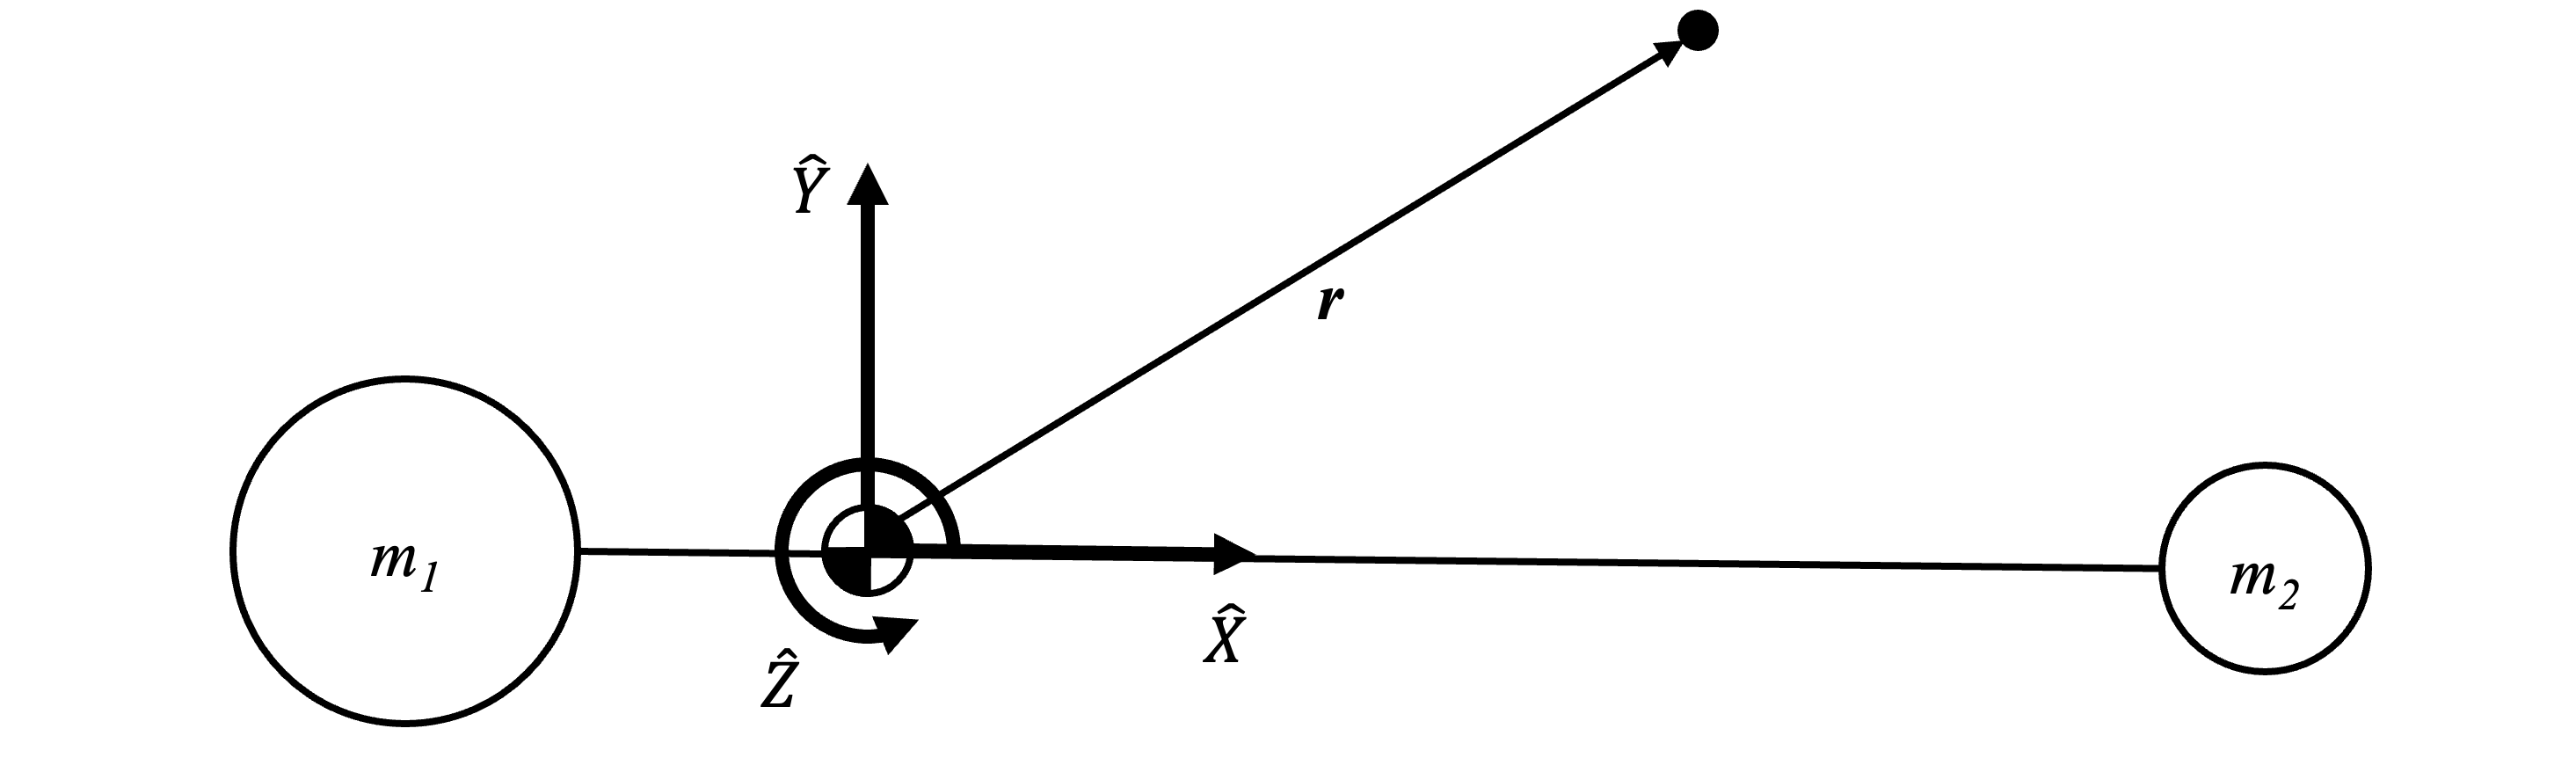
\includegraphics[width=1\linewidth]{Figures/CR3BP.png}
%     \caption{Circular-Restricted Three-Body Problem Coordinate Frame}
%     \label{fig:CR3BP}
% \end{figure}

Iannamorelli and LeGrand combine the adaptive Gaussian mixture and multiple model estimation approaches to simultaneously combat the extreme nonlinearity of cislunar dynamics and account for the maneuvers of a spacecraft \cite{iannamorelli2025adaptive}. Their adaptive Gaussian mixture interacting multiple model estimator (AGMIMM) models maneuvers as zero-mean, Gaussian process noise, so if properly tuned to capture all possible spacecraft maneuvers, the AGMIMM is able to accurately determine where the spacecraft \textit{could} be. However, it is reasonable to assume that the maneuvers of the target spacecraft will be optimal, in which case modeling maneuvers as zero-mean process noise would be overly-conservative. If instead some optimal control law is assumed, given observations of the beginning of a maneuver, it is possible to predict where the spacecraft \textit{should} be at some future time with less uncertainty than by modeling maneuvers as zero-mean process noise. As cislunar SDA becomes more complex with more cislunar spacecraft, decreasing this uncertainty will be critical for correlating tracks of multiple maneuvering targets and allocating limited observational resources.

The concept of using optimal control to improve tracking is explored by Holzinger et al., resulting in the development of the control-distance metric \cite{holzinger2012object}. The control-distance metric characterizes the amount of control effort required to connect two spacecraft states assuming some optimal control, thus allowing the correlation of tracks which are separated by smaller control distances. Lubey and Scheeres apply this framework to develop a sequential estimator, resulting in the Optimal Control-Based Estimator (OCBE) \cite{lubey2013optimal}. The OCBE models any deviation in the state dynamics as an optimal control, which allows both control inputs and mismodeled dynamics to be reconstructed from these deviations. The OCBE is applied by Greaves and Scheeres to the cislunar tracking problem for maneuver detection and reconstruction \cite{greaves2021observation}. These approaches, however, are for the posterior reconstruction and detection of maneuvers rather than for the prior prediction of maneuvers. 

The main contribution of this paper is the implementation of an assumed optimal control policy directly into the dynamics of an adaptive multiple-model estimator. An IMM with two modes is utilized, where the non-maneuvering (coasting) mode assumes ballistic dynamics, and the maneuvering (thrusting) mode assumes a minimum-time optimal control policy. The dynamics of the minimum-time optimal control policy are obtained using Pontryagin's minimum principle \cite{pontryagin1962}. This optimal control IMM (OCIMM) is used to track a cislunar spacecraft performing a low-thrust transfer between two periodic cislunar orbits under a fuel-optimal control policy, whose thrusting arcs follow the same dynamics of a time-optimal policy. The OCIMM is shown to be able to accurately predict the future control inputs of the target spacecraft, even during observation gaps and periods of rapidly changing control. This results in superior estimation performance compared to a traditional IMM. 


% Summary and/or conclusions are optional but often used.
% The summary and/or conclusions often are the last
% the last major division(s) of the text.
% Reference: TM2017 page 32.
\ProvidesFile{ch-summary.tex}[2022-10-05 summary chapter]

\begin{VerbatimOut}{z.out}
\chapter{SUMMARY}

This is the summary chapter.


\section{First Section}

This is the first section of the summary chapter.
\end{VerbatimOut}

\MyIO


% Recommendations are optional.
% You may include recommendations as a major division if your
% subject matter and research dictate.
% Reference: TM2017 page 32.
\ProvidesFile{ch-recommendations.tex}[2022-10-05 recommedations chapter]

\chapter{RECOMMENDATIONS}

Buy low.
Sell high.


% Test \begin{chapteracknowledgement}...\end{chapteracknowledgement}, etc.
%%%% \ProvidesFile{ch-test-miscellaneous.tex}[2023-09-06 test miscellaneous chapter]

\begin{refsection}

\chapter{TEST MISCELLANEOUS}

\newenvironment
  {chapteracknowledgement}%
  {%
    \bgroup
      \ZZbaselinestretch{1}%
      \vspace*{0.2\baselineskip}%
      \addtolength{\leftskip}{0.5in}%
      \addtolength{\rightskip}{0.5in}%
      \addtolength{\textwidth}{-1in}%
  }%
  {%
      \endgraf
      \vspace*{0.45\baselineskip}
    \egroup
  }
  
\begin{chapteracknowledgement}
  This was published in Mad Magazine.
  This was published in Mad Magazine.
  This was published in Mad Magazine.
  This was published in Mad Magazine.
  This was published in Mad Magazine.
  This was published in Mad Magazine.
  This was published in Mad Magazine.
  This was published in Mad Magazine.
  This was published in Mad Magazine.
  This was published in Mad Magazine.
  This was published in Mad Magazine.
  This was published in Mad Magazine.
  This was published in Mad Magazine.
  This was published in Mad Magazine.
  This was published in Mad Magazine.
\end{chapteracknowledgement}


This chapter is used to test miscellaneous stuff.  

\begin{covexample}
  This is a covexample test.
  This is a sentence.
  This is a sentence.
  This is a sentence.
  This is a sentence.
  This is a sentence.
  This is a sentence.
\end{covexample}

\begin{covexamples}
  \item
    This is a covexamples test.
    This is the first item.
    This is the first item.
    This is the first item.
    This is the first item.
    This is the first item.
  \item
    This is the secord item.\\
    This is the second item.
\end{covexamples}

This is an example of normal text.
This is an example of normal text.
This is an example of normal text.
This is an example of normal text.
This is an example of normal text.
This is an example of normal text.
This is an example of normal text.
This is an example of normal text.
This is an example of normal text.
This is an example of normal text.

\begin{definition}
  \ZZbaselinestretch{1.5}
  This is an example definition.
  This is an example definition.
  This is an example definition.
  This is an example definition.
  This is an example definition.
\end{definition}

This is an example of normal text.
This is an example of normal text.
This is an example of normal text.
This is an example of normal text.
This is an example of normal text.
This is an example of normal text.
This is an example of normal text.
This is an example of normal text.
This is an example of normal text.
This is an example of normal text.

\begin{observation}
  \ZZbaselinestretch{1.5}
  This is an example observation.
  This is an example observation.
  This is an example observation.
  This is an example observation.
  This is an example observation.
\end{observation}

This is an example of normal text.
This is an example of normal text.
This is an example of normal text.
This is an example of normal text.
This is an example of normal text.
This is an example of normal text.
This is an example of normal text.
This is an example of normal text.
This is an example of normal text.
This is an example of normal text.

\begin{proof}
  \ZZbaselinestretch{1.5}
  This is an example proof.
  This is an example proof.
  This is an example proof.
  This is an example proof.
  If \(a = b\) and \(b = c\) then \(a = c\).
\end{proof}

This is an example of normal text.
This is an example of normal text.
This is an example of normal text.
This is an example of normal text.
This is an example of normal text.
This is an example of normal text.
This is an example of normal text.
This is an example of normal text.
This is an example of normal text.
This is an example of normal text.

\begin{proposition}
  \ZZbaselinestretch{1.5}
  This is an example proposition.
  This is an example proposition.
  This is an example proposition.
  This is an example proposition.
  This is an example proposition.
\end{proposition}

This is an example of normal text.
This is an example of normal text.
This is an example of normal text.
This is an example of normal text.
This is an example of normal text.
This is an example of normal text.
This is an example of normal text.
This is an example of normal text.
This is an example of normal text.
This is an example of normal text.

\begin{theorem}
  \ZZbaselinestretch{1.5}
  This is an example theorem.
  This is an example theorem.
  This is an example theorem.
  This is an example theorem.
  This is an example theorem.
\end{theorem}

This is an example of normal text.
This is an example of normal text.
This is an example of normal text.
This is an example of normal text.
This is an example of normal text.
This is an example of normal text.
This is an example of normal text.
This is an example of normal text.
This is an example of normal text.
This is an example of normal text.

\begin{singlespace}
  \PrintChapterBibliography
\end{singlespace}

\end{refsection}


% Test per-chapter references.
%%%% \ProvidesFile{ch-test-per-chapter-references.tex}[2023-09-06 test per-chapter references]

% Use \begin{refsection} ... \end{refsection} to start/end per-chapter references.
\begin{refsection}

\chapter{TEST PER-CHAPTER REFERENCES}

\verb+\cite[page v]{knuth2012}+ gives ``\cite[page v]{knuth2012}''.

\noindent
\verb+\cite[back cover]{lamport1994}+ gives ``\cite[back cover]{lamport1994}''.

\noindent
\verb+\cite{thesis2017}+ gives ``\cite{thesis2017}''.

\noindent
\verb+\cite{thesis2020}+ gives ``\cite{thesis2020}''.

\noindent
\verb+\cite{t001}+ gives ``\cite{t001}''.

\noindent
\verb+\cite{t002}+ gives ``\cite{t002}''.

\noindent
\verb+\cite{t003}+ gives ``\cite{t003}''.

\noindent
\verb+\cite{t004}+ gives ``\cite{t004}''.

\noindent
\verb+\cite{t005}+ gives ``\cite{t005}''.

\noindent
\verb+\cite{t006}+ gives ``\cite{t006}''.

\begin{singlespace}
  \PrintChapterBibliography
\end{singlespace}

% Use \begin{refsection} ... \end{refsection} to start/end per-chapter references.
\end{refsection}


\makeatletter  % commented out on 2022-01-26
  \defbibenvironment{bibliography}
    {%
      \list
        {%
          \printtext[labelnumberwidth]%
          {%
            \printfield{prefixnumber}%
            \printfield{labelnumber}%
          }%
        }%
        {%
          \setlength{\bibhang}{1in} %%%%% was 0pt
          \setlength{\itemindent}{1in}%  -\leftmargin} %%%%% was 0pt
          \setlength{\itemsep}{\bibitemsep}%
          \setlength{\leftmargin}{0pt}%  .22in} % 0.42in}
          \setlength{\parsep}{\bibparsep}%
          \setlength{\rightmargin}{0.33in}%
        }%
    }
    {\endlist}
    {\item}
\makeatother  % commented out on 2022-01-26

% \immediate\setlength{\labelnumberwidth}{1.5in} %%%%% was commented out
\setlength{\labelwidth}{1.5in}

{%
  % Make _ in URLs visible.
  % \def\t{\char'137}%
  \catcode`*=\active
  \def*{\char'137}%  \char'137 is _
  \PrintBibliography
}

% Appendices are optional.  Not all theses contain appendices.
% An appendix is used for supplementary illustrative material,
% original data, computer programs, and other material that is not
% necessarily appropriate for inclusion within the text of your
% thesis.
% Reference: TM2017 page 33.
%
% Use ``\appendix'' for one appendix or ``\appendices'' for more than
% one appendix.
\appendices

% My filename conventions:
%     FILE THAT START WITH    ARE
%     ap-                     appendices
%     ch-                     chapters
%     gr-                     graphics
%     pa-                     packages
%     z                       temporary files

  % "About Appendices" appendix.
  \ProvidesFile{ap-about-appendices.tex}[2022-10-05 about the appendicies appendix]

\begin{VerbatimOut}{z.out}
\chapter{ABOUT THE APPENDICES}

% Use single spacing in the appendices from now on to save space.
\ZZbaselinestretch{1}

\textcolor{red}{%
  \textbf{%
    These appendices are single-spaced to save space.
    Your thesis should use the default~1.5 line spacing.%
  }%
}

There are two groups of appendices.
The first group are general appendices;
the second group are domain-specific appendices.

These appendices are a series of examples.
They are a work in progress.

Each example consists of some \LaTeX\ output
followed by the corresponding input lines.
Some \LaTeX\ input lines only define things
and don't produce any output.
Each chunk in the input file begins with
\verb+\begin{VerbatimOut}{z.out}+
then has the \LaTeX\ input for the example,
% Don't literally end VerbatimOut on next line.
and ends with {\tt \char'134 end\char'173 VerbatimOut\char'175},
followed by a blank line,
followed by a line that begins with
|\My|.

\end{VerbatimOut}

\MyIO


\begin{VerbatimOut}{z.out}


\section{Paragraphs}

This is the first paragraph.
Paragraphs are separated by blank lines.

This is the second paragraph.


\section{Section Heading}

This is a sentence.
This is a sentence.
This is a sentence.
This is a sentence.
This is a sentence.


\subsection{Subsection heading}

This is a sentence.
This is a sentence.
This is a sentence.
This is a sentence.
This is a sentence.


\subsubsection{Subsubsection heading}

This is a sentence.
This is a sentence.
This is a sentence.
This is a sentence.
This is a sentence.
\end{VerbatimOut}

\MyIO



\begin{VerbatimOut}{z.out}


\section{Text math}

If items in a list are narrow like these Greek characters,\\
    \I2 \verb+$\alpha$, $\beta$, and $\gamma$+\\
I'd input the line like this\\
    \I2 \verb+$\alpha$,~$\beta$, and~$\gamma$+\\
where the \verb+~+ is a tie
that ties together what's before and after it on the same line of the output
\cite[page~92]{knuth2012}.

This text is the correct length to show what happens with and without ties:
$\alpha$,
$\beta$,
and $\gamma$.
See how the line gets split
and the~$\gamma$ is at the beginning of the line?

This text is the correct length to show what happens with and without ties:
$\alpha$,~$\beta$,
and~$\gamma$.
See how the line gets compressed a little bit so the~$\gamma$
is not at the beginning of the line?
\end{VerbatimOut}

\MyIO


  % Accessibility.
  \ProvidesFile{ap-accessibility.tex}[2024-03-15 accessibility appendix]

\begin{VerbatimOut}{z.out}
\chapter{ACCESSIBILITY}
\ix{accessibility//Accessibility appendix}
\end{VerbatimOut}

\MyIO


\begin{VerbatimOut}{z.out}

Accessibility is the design of products,
devices,
services,
vehicles,
or environments
so as to be usable by people with disabilities.
\cite{wikipedia-accessibility}
\end{VerbatimOut}

\MyIO


\begin{VerbatimOut}{z.out}


\section{Color}

Color vision deficiency (CVD) affects more than 4\% of the population
and leads to a different visual perception of colors.
The cividis%
\ix{cividis colormap}
colormap is optimal
for viewing
by those with or without CVD
\cite{nunez2018}.
The
\citetitle{senn2022}
\cite{senn2022}
and
\citetitle{senn2022b}
\cite{senn2022b}
contain the Mathematica code used to produce this cividis example:\\[\baselineskip]
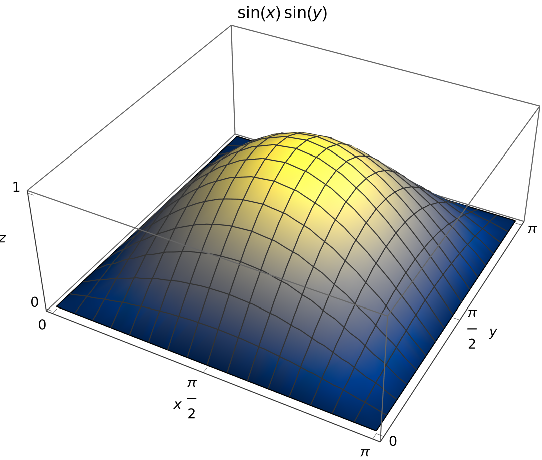
\includegraphics{gr-cividis.pdf}
\end{VerbatimOut}

Please use the cividis colormap for accessibility
unless there is a good reason not to.
\MyIO


\begin{VerbatimOut}{z.out}


\section{PDF file}

The \LaTeXLogo\ Project
\cite{thelatexproject2023}
is working on making tagged
and accessible PDF files with \LaTeXLogo\ %
\cite{mittlebach2022}.
It was not finished as of December 23, 2022.
\end{VerbatimOut}

\MyIO

  
  % "Bugs" appendix.
  \ProvidesFile{ap-bugs}[2025-01-28 bugs appendix]

\makeatletter
\newcommand{\bug}[2]
  {%
    \vspace{6pt}
    \noindent
    {%
      \bfseries
      \ifthen{\equal{high}{#2}}{\color{red}}%
      \ifthen{\equal{low}{#2}}{\color{blue}}%
      \ifthen{\equal{answered}{#2}}{\color{black}}%
      \ifthen{\equal{done}{#2}}{\color{black}}%
      \ifthen{\equal{fixed}{#2}}{\color{black}}%
      \ifthen{\equal{wait}{#2}}{\color{black}}%
      \ifthen{\equal{not}{#2}}{\color{gray}}%
      {\fontsize{9}{10}\reset@font\bf BUG}
      #1.
    }%
    \ignorespaces
  }
\makeatother

\chapter{BUGS}
\ix{bugs//Bugs appendix}

This appendix lists all bugs/comments/issues/etc\@.
under the generic name `bug'.
Each bug is assigned a number when I learn of it.
Bug numbers are 1, 2,~\ldots~.
I started keeping track of bugs in this fashion on February 26, 2022,
and some previously known bugs are included in this list.
A color indicates a bug's priority:

\begin{tabular}{@{}ll@{}}
  \toprule
  \bf Description& \bf Color\\
  \midrule
  done or waiting on someone else& \color{black}black\\
  high priority or easy to do& \color{red}red\\
  low priority& \color{blue}blue\\
  not prioritized yet& \color{gray}gray\\
  \bottomrule\\
\end{tabular}

See the
|ap-bugs.tex|
file
for the \LuaLaTeXLogo\ input
for this appendix.


\section{These bugs need to be looked at}

% I need to fix the following things in \PurdueThesis.
% They are listed in bug number order.

\bug{1}{high}
Table of Contents is double-spaced instead of 1\sfrac12 spacing.
{\small
  Tighten up section and less significant headings spacing?
  Reported by Anita Adams Sale on 2021-03-17.%
}

\bug{6}{not}
APA reference style indents references too far on left.
{\small
Reported by Mark Senn on 2021-04-08.%
}

\bug{8}{not}
Use, for example, |Last Accessed: yyyy-mm-dd.| urldate in bibliography.
{\small
  Reported by Mark Senn on 2021-04-19.%
}

\bug{13}{low}
Headings containing a SmallCaps font do not work.
{\small
  Reported by Javad (Nima) Darivandpour on 2021-06-29.
  See \ref{section-headings-with-smallcaps-font}.%
}

\bug{14}{low}
On Overleaf only,
when using
|\def\ZZshowtimestamp{true}|,
the time and sometimes the date
are wrong at the top of the page.
{\small
  Reported by Mark Senn on 2022-02-25.%
}

\bug{15}{not}
Left reference section margin is ok if a person has 10--99 references.
{\small
  Figure out how to adjusting margin for 1--9 or over 99 references.
  Reported by Mark Senn on unknown date.
}

\bug{19}{high}
|Bibliography| and |References| missing from navigation panel.
{\small
  Reported by Mark Senn on 2022-02-28.
  REFERENCES was in navigation panel on 2022-08-26.
}

\bug{20}{high}
|Bibliography| and |References| should be in all caps.
{\small
  Reported by Mark Senn on 2022-02-28.
  REFERENCES was in all caps on 2022-08-26.%
}

\bug{21}{low}
IE students should be able
to specify IEEE
or APA bibliography format.
{\small
  Reported by Patrick Brunese on 2022-03-04.%
}

\bug{24}{high}
Add |A Dissertation Proposal| document type.
Add |A Thesis Proposal| document type.
{\small
  Reported by Mark Senn on 2022-12-20.%
}

\bug{25}{high}
Dissertations and theses should continue to have
\Place{Month} \Place{year} where \Place{Month} is
|August|, |December|, or |May|.
For everything except dissertations and theses allow
\Place{Month} \Place{year}
or
\Place{Month} \Place{day}|, |\Place{year}
dates where \Place{Month} is any month.
{\small
  Reported by Mark Senn on 2022-12-20.%
}

\bug{26}{high}
Complete |HOW TO DEBUG| \LaTeX\ |PROBLEMS| chapter.
{\small
  Reported by Mark Senn on 2023-01-11.%
}

\bug{28}{high}
Move |\addbibresource|
from |PurdueThesis.cls|
to |thesis.tex|
to be more user friendly.
{\small
  Reported by Panos Manganaris on 2023-06-15.%  Panayotis Thalis Manganaris <pmangana@purdue.edu>
}

\bug{29}{high}
Main biblioography and chapter bibliography should be indented the same amount.
{\small
  Reported by Panos Manganaris on 2023-06-15.%  Panayotis Thalis Manganaris <pmangana@purdue.edu>
}

\bug{30}{low}
Main bibliography and chapter bibliography should both be flush with the left margin.
{\small
  Reported by Mark Senn on 2023-06-19.%
}

\bug{31}{high}
There needs to be way to put a list of publications in a publications section.
{\small
  Reported by Panos Manganaris on 2023-06-14.  %  Panayotis Thalis Manganaris <pmangana@purdue.edu>
  Mark Senn is working on a way to do that
  using
  |keywords = {publication}|
  in a \BibLaTeXLogo\ |.bib| file entry.
}

\bug{33}{low}
Create Color Vision Deficiency (CVD) Accessible Line Graphs.\\
{\small
  IEEE Author Center <ieee-author-center@deliver.ieee.org> wrote on 2024-03-20:
  \begin{quote}
    Approximately 1 in 12 men
    and 1 in 200 women
    have color vision deficiency.
    It is highly likely
    that someone reading your article
    may have difficulty distinguishing between red and green,
    blue and green,
    or yellow and red.
    The following tips will help you communicate better with those readers.
    \begin{itemize}
      \item
        Use both color and shape to convey the same meaning;
        for example,
        solid and dashed lines
        or different fill patterns can help readers understand the figure
        without relying solely on color
      \item
        Each line of your line graph
        should be a thick line with a unique data point symbol.
        Contrast different elements of the figure with both color and brightness
      \item
        Connect the data label
        to the data line
        rather than relying on a color key
    \end{itemize}
    A quick way to evaluate your figure is to print it out in greyscale
    and see if it can still be interpreted correctly;
    if not,
    use some of these tips to more effectively communicate with all readers.
  \end{quote}
  Lisa Renee Williams <will2922@purdue.edu> of the Graduate School wrote on 2024-03-21:
  \begin{quote}
    I think this is a wonderful idea and am in support of including information
    within the template to provide students the opportunity to use CVD.
  \end{quote}
}

\bug{34}{low}
Implement |\begin{chapterabstract}|
and |\end{chapterabstract}|
for abstracts within chapters.
Maybe rename this |paperabstract|?\\
{\small
  Reported by Mark Senn on 2024-04-09.
}

\bug{36}{low}
Improve the order of thesis parts error message
to indicate that not all parts listed are required.
{\small
  Reported by Mark Senn on 2022-09-21.%
}

\bug{37}{low}
Check the spacing after all chapter and non-chapter headings
for consistency.
{\small
  Reported by Mark Senn on 2020-02-28.%
}

\bug{38}{low}
Add short caption info to documentation.
{\small
  See
  \href{https://www-chicagomanualofstyle-org.ezproxy.lib.purdue.edu/book/ed17/part1/ch03/psec040.html}{Shortening captions for a list of illustrations}
  for a suggestion regarding this.
  To do this in \LaTeXLogo\ do\hfil\break
  \begin{quote}
    |\caption[short caption]{long caption}|
  \end{quote}
  Reported by Mark Senn on 2023-12-08.%
}

\bug{39}{low}
Page links for longtables don't link to right place
from List of Tables.
{\small
  Example: Table R.6.
  Reported by Tunazzina Islam on 2025-01-27.%
  {\it This may work with \(\text{hyperref.sty} > 7.01\text h\) in \TeXLiveLogo\ 2025.}
}


\section{These bugs are waiting on a reply from someone other than Mark Senn}

\bug{10}{wait}
Using
|linktoc = section|
does not work with captions with
|\frac|.
{\small
  Reported by Mark Senn on 2021-05-27.
  In the short-term,
  check with Ashlee Messersmith
  if {\tt linktoc = page} can be used.
  If that's ok make the change
  and look into changing captions from my code
  to \LaTeXLogo's code.
  Waiting on Ashlee Messersmith.
}


\section{These bugs have been answered, fixed, or rejected}

\bug{2}{done}
List of Figures indented $\approx$\sfrac14 inch
more than List of Tables.
{\small
  Reported by Anita Adams Sale on 2021-03-17.
  Still happening on 2021-11-30.
  Looked ok on 2022-08-26
  but I think this problem is probably intermittent.
  Keep Ashlee Messersmith,
  Anita Adams Sale,
  and Sherrie Tucker informed.
  Adam Behnke sent me the solution to this problem on 2023-03-27.
}

\bug{3}{done}
Use ``Last Accessed: dd/mm/yy.'' urldate in bibliography.
{\small
  Reported by Priyank Kalgaonkar on 2021-04-06.
  Answered by Mark Senn on 2022-02-27.

  The United States uses mm/dd/yy and other countries use dd/mm/yy
  \cite{cms17-ambiguous-dates}.
  I recommend using what your bibliography style defines
  or the unambiguous ISO 8601 standard yyyy-mm-dd
  \cite{cms17-iso-dates}.%
}

\bug{4}{done}
Change citation, e.g., |[6], [71]| to |[6,71]|.
{\small
  Reported by Mark Senn on 2021-04-07.
  Fixed on 2022-04-14.
  Tested ok on 2022-04-14.%
}

\bug{5}{done}
Change citation, e.g., |[6], [7], [8]| to |[6-8]|.
{\small
  Reported by Mark Senn on 2021-04-07.
  Fixed on 2022-04-14.
  Tested ok on 2022-04-14.%
}

\bug{7}{fixed}
Non-nested description environments have bold items.
Nested description environments have non-bold items.
How come?
Are the indentations correct?
{\small
  Reported by Mark Senn on 2021-04-09.
  Tested ok on 2021-05-31.%
}

\bug{9}{done}
Check that |@{}| is before the left column
and after the right column in all tables.
{\small
  Reported by Mark Senn on 2021-04-19.
  Tested ok on 2022-10-18 using\hfil\break
  \verb+alias g=grep+\hfil\break
  \verb+g -P '^\s*\\begin{tabular}' *.tex | g -Pv '^.*?:\s*\\begin{tabular}{@{}.*?@{}}'+%
}

\bug{11}{answered}
Bibliography change:
Change,
for example,
``Acoustical Science and Technology, vol.~23, no.~1''
to
``Acoustical Science and Technology {\bfseries 23\/} ({\bfseries 1\/})''.
{\small
  Reported by Daniel Joesph Carr on 2021-06-16.
  Answered by Mark Senn on 2022-10-18.

  The
  \citetitle{ieee-reference-guide}
  \cite[page~12]{ieee-reference-guide}
  specifies that |vol.|~and |no.|~should be used.
  You are the only one that has requested this.
  I'm not going to change anything because of that.
  I like the succinct ``{\bfseries 23\/} ({\bfseries 1\/})''
  format but am not going to implement it because not
  everyone will know those are the journal volume and number.
}

\bug{12}{answered}
Bibliography change:
Change,
for example,
{\tt M.~Abramowitz and I.A.~Stegun, Eds.,}
to
{\tt M.~Abramowitz and I.A.~Stegun, editors,}
{\small
  Reported by Daniel Joesph Carr on 2021-06-16.
  Answered by Mark Senn on 2022-10-18.

  The
  \citetitle{ieee-reference-guide}
  \cite[page~5]{ieee-reference-guide}
  specifies that |Ed.|~for a single editor
  and |Eds.|~for multiple editors be used.

  You are the only one that has requested this.
  I'm not going to change anything because of that.

  But,
  if you put the current ieee.bbx file
  in the same directory as your thesis
  and change
  \verb+editor = Ed\adddot+
  to
  \verb+editor = editor\adddot+
  and
  \verb+editors = Eds\adddot+
  to\hfil\break
  {\tt editors = editors\char'134 adddot}
  it may do what you want.
  Email
  |latex@ecn.purdue.edu|
  if you need the current ieee.bbx file.
  I have not tested this answer.
}

\bug{16}{fixed}
Add DTECH degree.
{\small
  Reported by Mark Senn on unknown date.
  Program ``Technology''
  and degree ``Doctor of Technology'' worked ok
  on 2022-08-26.%
}

\bug{17}{fixed}
Allow |,| (comma) in |\title|.
{\small
  Reported by Mark Senn on unknown date.
  Tested ok on 2021-11-30.%
}

\bug{18}{fixed}
Allow |\\| in |\title|.
{\small
  Reported by Mark Senn on unknown date.
  Tested ok on 2021-11-30.%
}

\bug{22}{fixed}
|\H{o}| works in
\pdfLaTeXLogo\ but does not work in \LuaLaTeXLogo.
{\small
  Reported by Raymond Polak III on 2022-10-28.
  Use |\H{o}| to get \H{o} in the text.
  Use |\ZZH{o}| to get \H{o} in the bibliography.
  Tested ok on 2023-03-27.%
}

\bug{23}{fixed}
The
|Department of Human Development and Family Studies|
was renamed to
|Department of Human Development and Family Science|.
{\small
  Reported by Mark Senn on 2022-12-03.
  Fixed on 2024-06-12.
}

\bug{27}{done}
The figures in subsections
\ref{ss:counter-example}
and
\ref{ss:fourier-transform-example}
are\\
\hbox to \hsize{
  \hss
  \begin{tabular}{@{}lll@{}}
    \toprule
    \bf Color& \bf On Operating Sytem& \bf Using\\
    \midrule
    color& macOS 12.6.2& Firefox 108.0.2 (64-bit)\\
    color& Ubuntu 22.04 LTS& evince (GNOME Document Viewer 42.3)\\
    black and white& Ubuntu 22.04 LTS& Firefox 108.0.2 (64-bit)\\
    \bottomrule
  \end{tabular}
  \hss
}\\
{\small
  Reported by Mark Senn on 2023-01-11.
  Use software that will show the colors correctly.%
}

\bug{32}{fixed}
The first two pages of the thesis
(the title page
and the graduate school statement of committee approval)
should have a top margin of 1 1/2 \si{\in}.
{\small
  Reported by Lisa Williams on 2023-12-08.
  % Lisa Williams <will2922@purdue.edu>
  Fixed on 2024-02-07.
  Tested ok on 2024-02-07.%
}

\bug{35}{done}
Is there an easy way of dividing the thesis into multiple parts?\\
{\small
  Asked by Vahid Tac on 2024-05-29.
  Thesis Help (Lisa Williams) <thesishelp@purdue.edu>
  wrote on 2024-06-04
  ``Since it is not part of the thesis structure in Purdue policies,
  we do not want parts\ldots''.%
  % See
  %   /home/pier/e/queue/Mail/archives/latex/YM2406/8
  % for the queue item and
  %   ~/PurdueThesis/template/part.tex
  % for notes on how to implement \part.
}



  % Check margins.
  \ProvidesFile{ap-check-margins.tex}[2022-10-05 check margins appendix]

\begin{VerbatimOut}{z.out}
\chapter{CHECK MARGINS}
\end{VerbatimOut}

\MyIO


\begin{VerbatimOut}{z.out}
\MyRepeat{This is a sentence. }{300}
\end{VerbatimOut}

\MyIO


  % Demonstrate how to do separate appendices per chapter.
  \ProvidesFile{ap-chapter-appendices.tex}[2022-10-05 chapter appendices appendix]

\begin{VerbatimOut}{z.out}
\chapter{CHAPTER APPENDICES}

Using |\chapterappendix|
or |\chapterappendices|
in a chapter will number sections,
for example,
1.1,
1.2,
\ldots,
1.A,
1.B,
\ldots\,.

Using |\chapterappendix|
or |\chapterappendices|
in an appendix will number sections,
for example,
A.1,
A.2,
\ldots,
A.A,
A.B,
\ldots\,.

I suggest only using |\chapterappendix|
or |\chapterappendices| in chapters---%
using them in appendices is too confusing.
\end{VerbatimOut}

\MyIO


\begin{VerbatimOut}{z.out}
\newpage


\section{This is a section heading}

This is a paragraph.

Use \verb+\chapterappendix+ or \verb+\chapterappendices+
to make sections until the end of the next chapter
be appendices.


\chapterappendix


\section{This is a chapter appendix}

This is a paragraph.
\end{VerbatimOut}

\MyIO


  % Citations and references.
  \ProvidesFile{ap-citations.tex}[2024-10-04 citations and references appendix]

\begin{VerbatimOut}{z.out}
\chapter{CITATIONS AND REFERENCES}
\end{VerbatimOut}

\MyIO


\begin{VerbatimOut}{z.out}

In your thesis try to cite only original sources like articles
and books.
If possible,
don`t use encyclopedias and Wikipedia.
\cite{citing-wikipedia}
\end{VerbatimOut}

\MyIO


\begin{VerbatimOut}{z.out}

This chapter contains information about citations
and references---how to cite a reference in the text
and the fine points of defining a bibliography
(also called ``References'')
entry.
\end{VerbatimOut}

\MyIO


\begin{VerbatimOut}{z.out}


\section{Citations}
\end{VerbatimOut}

\MyIO


\begin{VerbatimOut}{z.out}
This @online entry does not have a date
but has a urldate:
\cite{engineering}.

\citetitle{erdos1992}
by Paul Erd\H os
\cite{erdos1992}
was published in
\citeyear{erdos1992}.

For \LaTeX\ answers I refer to
\cite{lamport1994}
and then to
\cite{goossens1994}
or
\cite{kopka1999}.
\cite{kopka1999}
is an update to
\cite{kopka1995}.
\end{VerbatimOut}

\MyIO


\begin{VerbatimOut}{z.out}

Here is an example .bib file entry:

{\footnotesize
\begin{verbatim}
@misc{example2020,
  address   = {Imaginaryville, Indiana},
  author    = {Andrew Anteater and Bertha Bear and Charles Cheetah and Davida Deer
                and Ethan Eagle},
  date      = {2020-10-27},
  doi       = {00.0000/000-0-000-00000-0},
  editor    = {Mark Senn},
  edition   = {2},
  isbn      = {{000\FigureDash 0\FigureDash 000\FigureDash 00000\FigureDash 0}},
  publisher = {Bogus International Publishing Company},
  title     = {{Neil A.~Armstrong} Worked for {NASA}},
  url       = {https://bogus.com/bogus.html},
  urldate   = {2020-10-27},
  version   = {1.0},
}
\end{verbatim}
}
\end{VerbatimOut}

\MyIO


\begin{VerbatimOut}{z.out}

Below are some example |ieee| style \BibLaTeXLogo\ citations.
  
(%
  Different citation styles may give different results,
  for example,
  in the |apa| style,\\
  |\cite{example2020}|
  gives
  ``Anteater et al., 2020''
  and
  |\parencite{example2020}|
  gives
  ``(Anteater et al., 2020)''.
  See
  \cite{apa-style-examples}
  for more information.
  I'll document all the citation styles
  that \PurdueThesisLogo\ uses based on how
  |\ZZinstitution|,
  |\ZZcampus|,
  and |\ZZprogram| are set later.%
)

\begin{inlinetable}
  \begin{tabular}{@{}ll@{}}
    \toprule
    \textbf{Input}&                   \textbf{Output}\\
    \midrule
    \verb+\cite{example2020}+&        \cite{example2020}\\
    \verb+\cite*{example2020}+&       \cite*{example2020}\\
    \verb+\citeauthor{example2020}+&  \citeauthor{example2020}\\
    \verb+\citeauthor*{example2020}+& \citeauthor*{example2020}\\
    \verb+\citedate{example2020}+&    \citedate{example2020}\\
    \verb+\citetitle{example2020}+&   \citetitle{example2020}\\
    \verb+\citetitle*{example2020}+&  \citetitle*{example2020}\\
    \verb+\citeurl{example2020}+&     \citeurl{example2020}\\
    \verb+\citeyear{example2020}+&    \citeyear{example2020}\\
    \verb+\parencite{example2020}+&   \parencite{example2020}\\
    \verb+\textcite{example2020}+&    \textcite{example2020}\\
    \bottomrule
  \end{tabular}
\end{inlinetable}
\end{VerbatimOut}

\MyIO


  % Common mistakes.
  \ProvidesFile{ap-common-mistakes.tex}[2024-05-05 common mistakes appendix]

\begin{VerbatimOut}{z.out}
\chapter{COMMON MISTAKES}

The following Headings, Mathematics, and Text
sections describe some common mistakes.




\section{Headings}

\textcite[page~289]{farkas2011}
wrote

\begin{quotation}
  The practice of stacking headings
  is routinely condemned by style manuals
  and other authorities.
  Here is a typical statement,
  taken from Houghton Mifflin's guidelines for authors.
  \begin{quotation}
    Avoid ``stacking'' heads,
    or placing two levels
    of headings together without intervening text.
    A heading cannot substitute
    for the transitional
    or introductory paragraphs
    that guide the reader through a chapter.
    Remember too that a chapter opening looks better in type
    when one
    or more paragraphs
    of text precede the first heading.
  \end{quotation}
\end{quotation}
\end{VerbatimOut}

\MyIO


\begin{VerbatimOut}{z.out}


\section{Mathematics}

\subsection{Put a little extra horizontal space before dx}
\end{VerbatimOut}
\MyIO


\begin{VerbatimOut}{z.out}


\section{Text}
\end{VerbatimOut}

\MyIO


\begin{VerbatimOut}{z.out}

\subsection{e.g.,}
\ix{e.g.}

``e.g.'' should always be followed by a comma.
\end{VerbatimOut}

\MyIO


\begin{VerbatimOut}{z.out}

\subsection{``et al.'' is an abbreviation}
\ix{et al.}

The phrase ``et al.''
is an abbreviation
and should always be followed by a period.
It should be in the normal font for your document---%
do not italicize or underline it.

Example:\\[6pt]
\indent\indent
\begin{tabular}{@{}ll@{}}
  input&   \verb+Thun et al.~used data from Santa Claus.+\\
  output&  Thun et al.~used data from Santa Claus.\\
  comment& my recommendation\\[6pt]
  input&   \verb+Thun et al. used data from Santa Claus.+\\
  output&  Thun et al. used data from Santa Claus.\\
  comment& too much space after period---\LaTeX\ thinks period is end of sentence\\[6pt]
  input&   \verb+Thun et al\@. used data from Santa Claus.+\\
  output&  Thun et al\@. used data from Santa Claus.\\
  comment& spacing is right but the ``et al.'' could occur at end of a line\\
\end{tabular}
\end{VerbatimOut}

\MyIO


\begin{VerbatimOut}{z.out}

\subsection{i.e.,}
\ix{i.e.}

``i.e.'' should always be followed by a comma.
\end{VerbatimOut}

\MyIO


\begin{VerbatimOut}{z.out}

\subsection{ldots}

Use ``1, 2, \ldots, 10''
instead of 1, 2, ..., 10''
\end{VerbatimOut}

\MyIO


\begin{VerbatimOut}{z.out}

\subsection{text math subscripts}

If you are using an English word
as a math subscript or subsubscript
typeset it in a roman font like this
`\(x_\text{max}\)'
instead of
`\(x_{max}\)'.
\end{VerbatimOut}

\MyIO


\begin{VerbatimOut}{z.out}

\subsection{ties}

Change the space in
`Dr. ', `Fig. ', `Mr. ', `Mrs. ', `Mx. ', `Prof. ', etc.,
to `\(\sim\)' so the period will only be followed by one
space and, for example, `Dr.' and `Smith' will be tied
together so they won't be split over two lines.
\end{VerbatimOut}

\MyIO


  % Defining commands.
  \ProvidesFile{ap-defining-commands.tex}[2022-10-05 defining commands appendix]

\begin{VerbatimOut}{z.out}
\chapter{DEFINING COMMANDS}

The next paragraph demonstrates how to define and use a command.

\renewcommand{\t}[2]
{% The "{%" hides the space caused by the newline.  LaTeX ignores leading spaces on a line.
  Editors recommend that a #1 should never be
  followed by a #2 without some intervening text.
}

\t{chapter title}{section heading}
I suggest writing for readers.
Break the rules if necessary.
\end{VerbatimOut}

\MyIO


  % Deprecated software.
  \ProvidesFile{ap-deprecated-software.tex}[2023-02-06 ap-deprecated-software appendix]

\begin{VerbatimOut}{z.out}
\chapter{DEPRECATED SOFTWARE}

Deprecated means
\cite{merriam-webster-deprecated}
\begin{quote}
  to withdraw official support for or discourage the use of
  (something, such as a software product)
  in favor of a newer or better alternative.
\end{quote}

The following software is deprecated for use with \PurdueThesisLogo.
Read the ``Details''
or ``Used For''
columns below for more information.
\end{VerbatimOut}

\MyIO


\begin{VerbatimOut}{z.out}


\section{Bibliography Software}

\noindent
\begin{tabularx}{\textwidth}{@{}lX@{}}
  \toprule
  \bf Software Name& \bf Details\\
  \midrule
  Mendeley&
    If you don't currently use Mendeley
    and are thinking about using Mendeley just for your thesis
    I suggest that you do not do it.
    It may cause more problems than it solves.
    You can type the data needed for your bibliography
    directly into .bib files.\\
  \bottomrule
\end{tabularx}
\end{VerbatimOut}

\MyIO


\begin{VerbatimOut}{z.out}


\section{Packages}

The
|\usepackage{|\Place{packagename}|}|
command is used to load a package.

Do not use these packages---they are not compatible with \PurdueThesisLogo.\\

\noindent
\begin{tabularx}{\textwidth}{@{}lX@{}}
  \toprule
  \bf Package Name& \bf Used For\\
  \midrule
  babel&
    Translating ``Table of Contents'', etc\@. to foreign languages.
    Reported by Danushka Menikkumbura.
    Send email to \verb+latex@ecn.purdue.edu+ if you need to
    typset multiple languages in your thesis.\\
  caption&
    Used to customize captions.
    Do not load this package, it is not compatible with \PurdueThesisLogo.\\
  glossaries&
    Used to make glossaries.
    Do not load this package, it is not compatible with \PurdueThesisLogo.
    See the \verb+front.tex+ file for haw to make a glossary.\\
  glossary&
    For glossararies.
    This package is deprecated.
    Do not load this package.
    See \verb+glossaries+.\\
      subfig&
    For subfigures.
    This package is deprecated.
    Do not load this package.
    See page \pageref{pa:subfigures} for how to do subfigures.\\
  subfigure&
    For subfigures.
    This package is deprecated.
    Do not load this package.
    See page \pageref{pa:subfigures} for how to do subfigures.\\
  \bottomrule
\end{tabularx}
\end{VerbatimOut}

\MyIO



  % Figures.
  \ProvidesFile{ap-figures.tex}[2025-01-16 figures appendix]

\begin{VerbatimOut}{z.out}
\chapter{FIGURES}
\end{VerbatimOut}

\MyIO


\begin{VerbatimOut}{z.out}

The
\verb+h+
specifier used in all the examples below
tells \LaTeX\ to put the figure
``here''
instead of trying
to find a good spot
at the top or bottom of a page.
Specifiers can be combined,
for example,
``\verb+\begin{figure}[htbp!]+''.
\end{VerbatimOut}

\MyIO


\begin{VerbatimOut}{z.out}

The complete list of figure placement specifiers:
\vspace*{6pt}
\begin{center}
  \begin{tabular}{@{}ll@{}}
    \toprule
    \bf Specifier& \bf Description\\
    \midrule
    \noalign{\vspace*{2pt}}
    \tt b& bottom of page\\
    \tt h& follow formatting rules and put here on page\\
    \tt p& on separate page of figures\\
    \tt t& top of page\\
    \tt !& try hard to put figure as early as possible\\
    \tt H& suspend formatting rules and put right here---requires \tt\char'134 usepackage\char'173 float\char'175\\
    \bottomrule
  \end{tabular}
\end{center}
\index{figure!placement specifiers (\verb+b+, \verb+h+, \verb+p+, \verb+t+, {\tt\char'041}, \verb+H+)}
\index{\verb+\begin{tabular}+}
\end{VerbatimOut}

\MyIO


% !!!! Label ``fi:not-centered'' is ``\ref{fi:not-centered}''.
% !!!! Label ``sf:four-parts-c'' is ``\ref{sf:four-parts-c}''.

\begin{VerbatimOut}{z.out}

% MyRepeat is defined in MyRepeat.sty.
\MyRepeat{This is the first paragraph.  }{5}
\end{VerbatimOut}

\MyIO


\begin{VerbatimOut}{z.out}

\begin{figure}[h]
  This is the figure.
  \caption{%
    Allocation to Common Edge for
    \(p(x_i) = 1-e^{-x_iz}\)% \frac{-x_i}z}\)%
  }
\end{figure}
\end{VerbatimOut}

\MyIO


\begin{VerbatimOut}{z.out}

\begin{sidewaysfigure}[ht]
  \setbox0=\hbox{%
    \noindent
    This is the second figure in this appendix.
    This is the second figure in this appendix.
    This is%
  }
  \dimen0=\wd0
  \hbox to \textwidth{\hss\box0\hss}
  \textwidth=\dimen0
  \advance\textwidth by 1truein
  \caption{%
    This is the caption for the second figure.
    This is the caption for the second figure.
    This is the caption for the second figure.%
  }
\end{sidewaysfigure}
\end{VerbatimOut}

\MyIO


\begin{VerbatimOut}{z.out}

\begin{sidewaysfigure}[ht]
  \setbox0=\hbox{\noindent 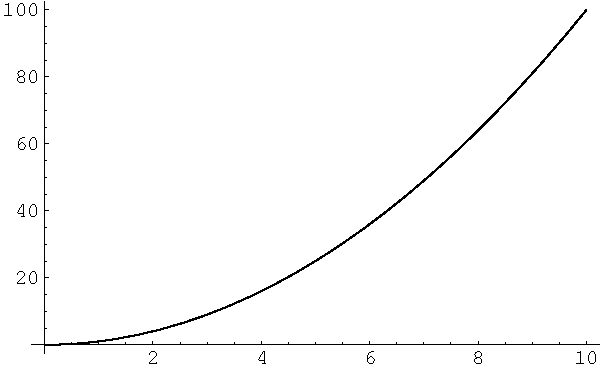
\includegraphics[width=8truein]{gr-plot.pdf}}
  \dimen0=\wd0
  \hbox to \textwidth{\hss\box0\hss}
  \textwidth=\dimen0
  \advance\textwidth by 1truein
  \caption{
    This is the caption for the third figure.
    This is the caption for the third figure.
    This is the caption for the third figure.%
  }
\end{sidewaysfigure}
\end{VerbatimOut}

\MyIO


\begin{VerbatimOut}{z.out}

\begin{figure}[ht]
  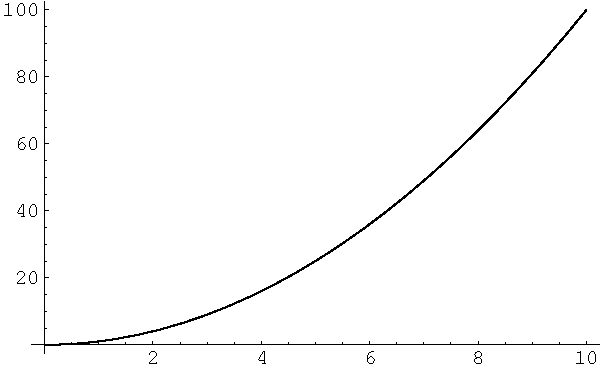
\includegraphics{gr-plot.pdf}
  \caption
  {%
    By default figures are not centered.
    This is a long caption to demonstrate that captions are single spaced.
    This is a long caption to demonstrate that captions are single spaced.%
  }
  \label{fi:not-centered}
\end{figure}
\end{VerbatimOut}

\MyIO


\begin{VerbatimOut}{z.out}

\MyRepeat{This is the second paragraph.  }{10}
\end{VerbatimOut}

\MyIO


\begin{VerbatimOut}{z.out}

\begin{figure}[ht]
  \centering
  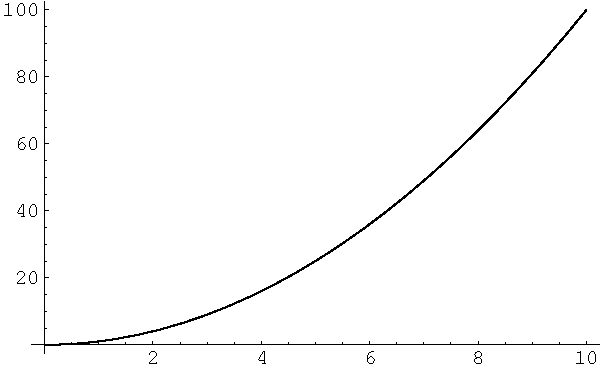
\includegraphics{gr-plot.pdf}
  \caption{Use {\tt \char'134centering\/} to center figures.}
  \label{fi:centered}
\end{figure}
\end{VerbatimOut}

\MyIO


\begin{VerbatimOut}{z.out}

\MyRepeat{This is the third paragraph.  }{15}
\end{VerbatimOut}

\MyIO


\begin{VerbatimOut}{z.out}

\begin{figure}[ht]
  \centering
  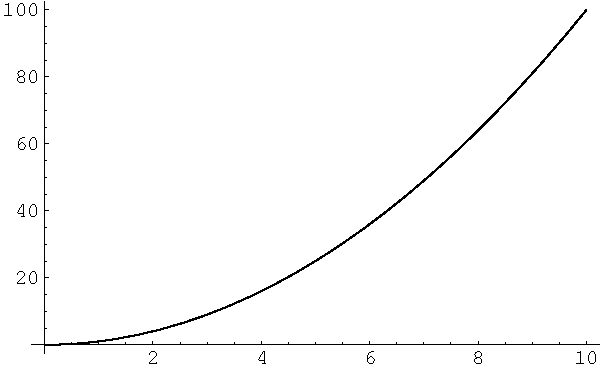
\includegraphics{gr-plot.pdf}
  \caption{This is another figuure.}
  \label{fi:another}
\end{figure}
\end{VerbatimOut}

\MyIO


\begin{VerbatimOut}{z.out}

\MyRepeat{This is the fourth paragraph.  }{10}
\end{VerbatimOut}

\MyIO


\begin{VerbatimOut}{z.out}
  
% See pages 4--5 of
%   http://mirrors.ibiblio.org/CTAN/macros/latex/contrib/caption/subcaption.pdf
% for how to use \subcaptionbox.
\begin{figure}[ht]
  % Center the entire figure (containing the two subfigures).
  \centering 
    % The \subcaptionbox for the first subfigure.
    \subcaptionbox
      % The first subcaption with a \label.
      % Use \ref{sf:two-parts-a} to print the subcaption number.
      {First subcaption.\label{sf:two-parts-a}}%
      % The first subfigure is this wide.
      [2in]%
      % This is the first subfigure.
      % You'll usually use an \includegraphics{filename}
      % inside the braces on the next line.
      {\bfseries First subfigure.}%
    % Put 0.5 inches of blank space between the subfigures.
    \hskip 0.5truein
    \subcaptionbox
      {Second subcaption.\label{sf:two-parts-b}}%
      [2in]%
      {\bfseries Second subfigure.}%
    % The caption for the entire figure (containing two subfigures).
    \caption{This figure has two subfigures arranged horizontally.}
    % The label for the entire figure.
    \label{fi:two-horizontal-parts}
\end{figure}
\ix{figure!subfigures!\(\text{1 row} \times \text{2 columns}\)}
\end{VerbatimOut}

\label{pa:subfigures}

\MyIO


\begin{VerbatimOut}{z.out}

\MyRepeat{This is the fifth paragraph.  }{10}
\end{VerbatimOut}

\MyIO


\begin{VerbatimOut}{z.out}

% See pages 4--5 of
%   http://mirrors.ibiblio.org/CTAN/macros/latex/contrib/caption/subcaption.pdf
% for how to use \subcaptionbox.
\begin{figure}[ht]
  % Center the entire figure (containing the two subfigures).
  \centering
    % The \subcaptionbox for the first subfigure.
    \vbox{\subcaptionbox  % use \vbox to stack subcaption boxes vertically
      % The first subcaption with a \label.
      % Use \ref{sf:two-vertical-parts-a} to print the subcaption number.
      {First subcaption.\label{sf:two-vertical-parts-a}}
      [2in]%
      {\bfseries First subfigure.}}%
    % Put \baselineskip blank space between the subfigures.
    \vspace*{\baselineskip}
    % The \subcaptionbox for the second subfigure.
    \vbox{\subcaptionbox  % use \vbox to stack subcaption boxes vertically
      {Second subcaption.\label{sf:two-vertical-parts-b}}
      [2in]%
      {\bfseries Second subfigure.}}%
  \caption{This figure has two subfigures arranged vertically.}
  \label{fi:two-vertical-parts}
\end{figure}
\ix{figure!subfigures!\(\text{2 rows} \times \text{1 column}\)}
\end{VerbatimOut}

\MyIO


\begin{VerbatimOut}{z.out}

\MyRepeat{This is the sixth paragraph.  }{10}
\end{VerbatimOut}

\MyIO


\begin{VerbatimOut}{z.out}
  
% See pages 4--5 of
%   http://mirrors.ibiblio.org/CTAN/macros/latex/contrib/caption/subcaption.pdf
% for how to use \subcaptionbox.
\begin{figure}[ht]
  \centering
    \subcaptionbox
      {First subcaption.\label{sf:four-parts-a}}
      [2in]%
      {\bfseries First subfigure.}%
    \hskip 0.5truein
    \subcaptionbox
      {Second subcaption.\label{sf:four-parts-b}}
      [2in]%
      {\bfseries Second subfigure.}%
    \vspace*{\baselineskip}
    \subcaptionbox
      {Third subcaption.\label{sf:four-parts-c}}
      [2in]%
      {\bfseries Third subfigure.}%
    \hskip 0.5truein
    \subcaptionbox
      {Fourth subcaption.\label{sf:four-parts-d}}
      [2in]%
      {\bfseries Fourth subfigure.}%
  \caption{This figure has four parts.}
  \label{fi:four-parts}
\end{figure}
\ix{figure!subfigures!\(\text{2 rows} \times \text{2 columns}\)}
\end{VerbatimOut}

\MyIO


\begin{VerbatimOut}{z.out}

\MyRepeat{This is the seventh paragraph.  }{10}
\end{VerbatimOut}

\MyIO


\begin{VerbatimOut}{z.out}

\newpage

\begin{figure}[ht]
  \centering 
    % Use a 5" font.
    {\fontsize{5in}{5in}\selectfont\(\hspace*{-0.07em}\sqrt 2\)}
    \caption{%
      A big ``\(\sqrt 2\)''.
      \LaTeX\ can make output big enough for T-shirts or posters.
      Square roots are printed with space before them,
      I put some negative horizontal space before this one to center it.%
    }
\end{figure}
\ix{figure!\(\sqrt 2\)}
\end{VerbatimOut}

\MyIO

\UndefineShortVerb{\|}  % so "|" in not a special character
\ix{subfigure|see{figure, subfigures}}
\DefineShortVerb{\|}  % so "|verbatim|" will be verbatim


\begin{figure}
  This is the figure.
  \caption{%
    Allocation to Common Edge for
    \(p(x_i) = 1-e^{-x_iz}\)% \frac{-x_i}z}\)%
  }
\end{figure}

\begin{VerbatimOut}{z.out}

\newpage

The remainder of this file tests having lots of figures.
There are 20 figures in this test.

\begin{figure}[ht]
  \centering
  
\includegraphics[scale=0.5]{gr-metapost-tally-01.pdf}
  \caption{Test figure 1 of 20.}
  \label{fi:1of20}
\end{figure}

\begin{figure}[ht]
  \centering
  
\includegraphics[scale=0.5]{gr-metapost-tally-02.pdf}
  \caption{Test figure 2 of 20.}
  \label{fi:2of20}
\end{figure}

\begin{figure}[ht]
  \centering
  
\includegraphics[scale=0.5]{gr-metapost-tally-03.pdf}
  \caption{Test figure 3 of 20.}
  \label{fi:3of20}
\end{figure}

\begin{figure}[ht]
  \centering
  
\includegraphics[scale=0.5]{gr-metapost-tally-04.pdf}
  \caption{Test figure 4 of 20.}
  \label{fi:4of20}
\end{figure}

\begin{figure}[ht]
  \centering
  
\includegraphics[scale=0.5]{gr-metapost-tally-05.pdf}
  \caption{Test figure 5 of 20.}
  \label{fi:5of20}
\end{figure}

\begin{figure}[ht]
  \centering
  
\includegraphics[scale=0.5]{gr-metapost-tally-06.pdf}
  \caption{Test figure 6 of 20.}
  \label{fi:6of20}
\end{figure}

\begin{figure}[ht]
  \centering
  
\includegraphics[scale=0.5]{gr-metapost-tally-07.pdf}
  \caption{Test figure 7 of 20.}
  \label{fi:7of20centered7}
\end{figure}

\begin{figure}[ht]
  \centering
  
\includegraphics[scale=0.5]{gr-metapost-tally-08.pdf}
  \caption{Test figure 8 of 20.}
  \label{fi:8of20}
\end{figure}

\begin{figure}[ht]
  \centering
  
\includegraphics[scale=0.5]{gr-metapost-tally-09.pdf}
  \caption{Test figure 9 of 20.}
  \label{fi:9of20}
\end{figure}

\begin{figure}[ht]
  \centering
  
\includegraphics[scale=0.5]{gr-metapost-tally-10.pdf}
  \caption{Test figure 10 of 20.}
  \label{fi:10of20}
\end{figure}

\begin{figure}[ht]
  \centering
  
\includegraphics[scale=0.5]{gr-metapost-tally-11.pdf}
  \caption{Test figure 11 of 20.}
  \label{fi:11of20}
\end{figure}

\begin{figure}[ht]
  \centering
  
\includegraphics[scale=0.5]{gr-metapost-tally-12.pdf}
  \caption{Test figure 12 of 20.}
  \label{fi:12of20}
\end{figure}

\begin{figure}[ht]
  \centering
  
\includegraphics[scale=0.5]{gr-metapost-tally-13.pdf}
  \caption{Test figure 13 of 20.}
  \label{fi:13of20}
\end{figure}

\begin{figure}[ht]
  \centering
  
\includegraphics[scale=0.5]{gr-metapost-tally-14.pdf}
  \caption{Test figure 14 of 20.}
  \label{fi:14of20}
\end{figure}

\begin{figure}[ht]
  \centering
  
\includegraphics[scale=0.5]{gr-metapost-tally-15.pdf}
  \caption{Test figure 15 of 20.}
  \label{fi:15of20}
\end{figure}

\begin{figure}[ht]
  \centering
  
\includegraphics[scale=0.5]{gr-metapost-tally-16.pdf}
  \caption{Test figure 16 of 20.}
  \label{fi:16of20}
\end{figure}

\begin{figure}[ht]
  \centering
  
\includegraphics[scale=0.5]{gr-metapost-tally-17.pdf}
  \caption{Test figure 17 of 20.}
  \label{fi:17of20}
\end{figure}

\begin{figure}[ht]
  \centering
  
\includegraphics[scale=0.5]{gr-metapost-tally-18.pdf}
  \caption{Test figure 18 of 20.}
  \label{fi:18of20}
\end{figure}

\begin{figure}[ht]
  \centering
  
\includegraphics[scale=0.5]{gr-metapost-tally-19.pdf}
  \caption{Test figure 19 of 20.}
  \label{fi:19of20}
\end{figure}

\begin{figure}[ht]
  \centering
  
\includegraphics[scale=0.5]{gr-metapost-tally-20.pdf}
  \caption{Test figure 20 of 20.}
  \label{fi:20of20}
\end{figure}
\end{VerbatimOut}

\MyIO


  % Frequently Asked Questions.
  \ProvidesFile{ap-frequently-asked-questions}[2024-10-31 frequently asked questions appendix]

\newcommand{\MyA}{\textbf{A: }}

\makeatletter
\newcommand{\faq}[2]
  {%
    \vspace{6pt}
    \noindent
    {%
      \bfseries
      \ifthen{\equal{high}{#2}}{\color{red}}%
      \ifthen{\equal{low}{#2}}{\color{blue}}%
      \ifthen{\equal{answered}{#2}}{\color{black}}%
      \ifthen{\equal{done}{#2}}{\color{black}}%
      \ifthen{\equal{fixed}{#2}}{\color{black}}%
      \ifthen{\equal{wait}{#2}}{\color{black}}%
      \ifthen{\equal{not}{#2}}{\color{gray}}%
      {\fontsize{9}{10}\reset@font\bf FAQ}
      #1.
    }%
    \ignorespaces
  }
\makeatother
  
\chapter{FREQUENTLY ASKED QUESTIONS}

This appendix lists all frequently asked questions.
Each frequently asked question is assigned a number when I learn of it.
FAQ numbers are 1, 2,~\ldots\,.
I started keeping track
of frequently asked questions
in this fashion
on March 1, 2022.

\begin{tabular}{@{}ll@{}}
  \toprule
  \bf Description& \bf Color\\
  \midrule
  done or waiting on someone else& \color{black}black\\
  high priority or easy to do& \color{red}red\\
  low priority& \color{blue}blue\\
  not prioritized yet& \color{gray}gray\\
  \bottomrule\\
\end{tabular}

See the
|ap-frequently-asked-questions.tex|
file
for the \LuaLaTeXLogo\ input
for this appendix.


\section{These questions need to be answered}


\section{These questions are waiting on a reply from someone other than Mark Senn}


\section{These questions have been answered}

The subsection headings below are what part of the document
the question is about.


\subsection*{Everywhere}
\faq{1}{done}
The \LaTeXLogo\ input\\
\I2 \verb+$a | b$+\qquad
(Mark Senn recommends using \verb+\(a | b\)+ instead)\\
%   {\tt\char'134(\$a \char'174\ \$b\char'134)}
%   instead%
% )\\
gives\\
\I2 |! LaTeX Error: Command \ttfamily invalid in math mode.|\\
Reported by Negin Karisani.\\
\MyA
In thesis.tex, change\\
\I2 \verb+\DefineShortVerb{\|} % so "|verbatim|" will be verbatim+\\
% {\tt
%   \char'134 DefineShortVerb%
%   \{\char'134\char'174\}\ \ %
%   \% so "\char'174 verbatim\char'174" will be verbatim%
% }\\
to\\
\I2 \verb+% \DefineShortVerb{\|} % so "|verbatim|" will be verbatim+
% {\tt
%   \%\ \char'134 DefineShortVerb%
%   \{\char'134\char'174\}\ \ %
%   \% so "\char'174 verbatim\char'174" will be verbatim%
% }


\faq{5}{done}
When using Overleaf on Firefox
I get a gratuitous `\Box'
in the upper-left corner of each page.\\
\MyA
Resetting Firefox
(warning: this resets lots of stuff)
using the following steps
worked for me:\\
\I2 1. Select \Menu{Help > Troubleshoot Mode}.\\
\I2 2. Click \Keys{Restart}.\\
\I2 3. Click \Keys{Refresh Firefox}.\\
\I2 4. Click \Keys{Refresh Firefox}.\\
\I2 5. Click \Keys{Let's Go}.


\subsection*{Table of Contents}

\faq{2}{done}
I want text instead of page number to be the link
in the table of contents.
Asked by Danushka Menikkumbura on 2022-03-11.\\
\MyA
In PurdueThesis.cls change \verb+linktoc = page+
to \verb+linktoc = section+.
I do not recommend doing this because
\begin{itemize}
  \item
    you'll need to put this change
    in new PurdueThesis.cls files in the future
  \item
    people are used to using page numbers instead
    of chapter/section/etc.~titles for where they
    start
\end{itemize}


\subsection*{Chapters}
\faq{6}{done}
Sections are numbered 2.1, 2.2, 2.3, 2.1 using |\chapterappendix|.
They should be numbered 2.1, 2.2, 2.3, 2.A.
How do I fix this?
Asked by Ryan Hastings on 2024-10-28.\\
\MyA                                                                                    
Change\\
\I2|\chapterappendix|\\
to\\
\I2|\chapterappendix|\\
\I2|\renewcommand{\thesection}{\thechapter.\AlphAlph{\value{section}}}|
                                                                                    
This was fixed in the new PurdueThesis software
that was put on Overleaf
around October 25, 2024.
It contains lots of changes
but I suggest you do not update to it
if you plan to graduate in December 2024---%
you'd need to read and make some updates to your
PurdueThesis.cls, thesis.tex, and front.tex files.                                  


\subsection*{References}
\faq{4}{done}
I have an
|@online{|\ldots
reference with no
|date = {|\ldots|}|
and `()' gets printed in the references
around where the date would go.
How can I prevent the `()'
from getting printed.
Asked by Pratith Narasimha Shenai on 2023-07-15.
\MyA
Use
|@online[*]{|\ldots
instead of
|@online{|\ldots\,.
I don't know why this works.


\subsection*{Appendix}

\faq{3}{done}
Label Appendix/Appendices with APPENDIX.
Asked by Panos Manganaris % Panayotis Thalis Manganaris <pmangana@purdue.edu>
on 2023-06-16.
\MyA
Mark Jaeger,
former Manager
of the Thesis and Dissertation Office,
wrote and said
that the most important thing
in a thesis was
`consistency,
consistency,
consistency'.

For consistency,
\begin{itemize}
  \item
    Chapters aren't labeled with `CHAPTER'
    so
    Appendix/Appendices aren't labeled with `APPENDIX'.
  \item
    Chapters are listed as 1,~2,~\ldots\ %
    and appendices are listed as A,~B,~\ldots\ %
    in the Table of Contents.
\end{itemize}

Contemporary usage is to not label
chapters or appendices see MIT theses
\cite{jiang2022,stehr2022},
Stanford theses
\cite{guikema2004,simper2022},
and \TeXLogo/\LaTeXLogo documentation
\cite{kime2022,knuth2012,lamport1994}.
% Lisa Williams <will2922@purdue.edu> wrote on 2023-06-27 at 14:59-04:
% Appendix headings are on the list to discuss for consistency.


  % Graphics.
  \ProvidesFile{ap-graphics.tex}[2024-05-31 graphics appendix]

\begin{VerbatimOut}{z.out}
\chapter{GRAPHICS}

There are many ways to make graphics for \LaTeX.
I like to use a system that uses \LaTeX\ fonts
so the appearance of the output is professional.
\end{VerbatimOut}

\MyIO


\begin{VerbatimOut}{z.out}

\section{MATLAB programming language}
\ix{MATLAB programming language}

\def\gray#1{\colorbox{gray!15}{#1}}
\def\lightred#1{\colorbox{red!15}{#1}}
\def\lightgreen#1{\colorbox{green!20}{#1}}
\lightgreen{%
  By default,
  MATLAB supports a subset of TeX markup
  \cite{mathworks-help-center-text-properties}.
}

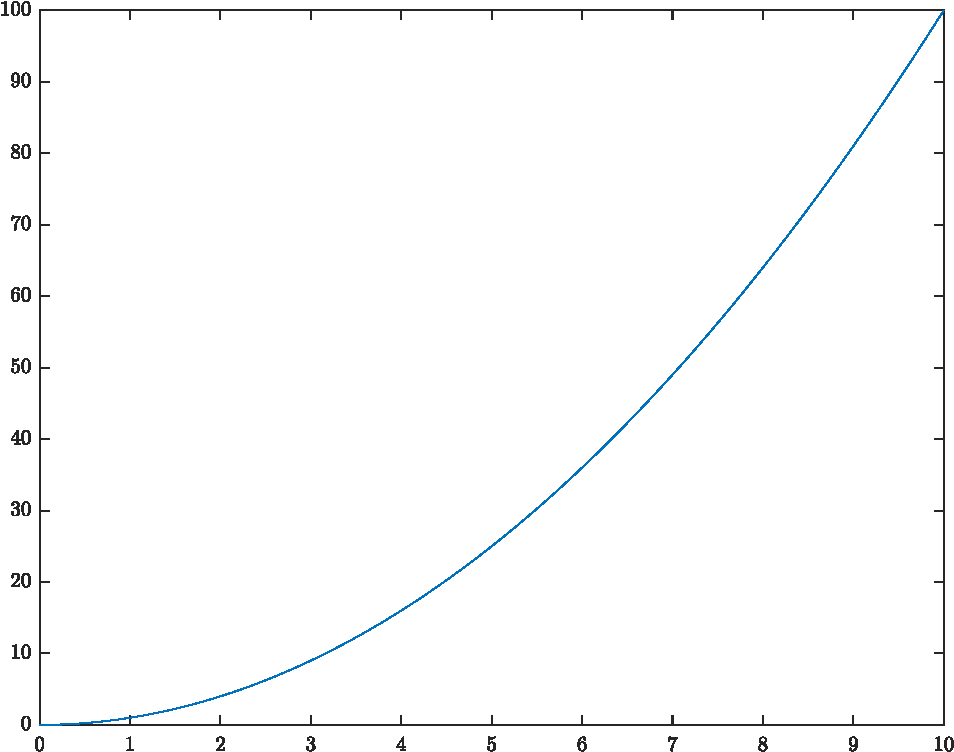
\includegraphics{gr-matlab.pdf}

This is the |misc/gr_matlab.m| input file:
\MyI{misc/gr_matlab.m}

I typed, on Linux,
\Shell{matlab -nodisplay -nodesktop -nosplash -r gr\_matlab}
in the |misc| subdirectory
to make the |graphics/gr-matlab.pdf| output file.
\end{VerbatimOut}

\MyIO


\begin{VerbatimOut}{z.out}

\section{\protect\METAPOSTLogo\ programming language}
\index{METAPOST@\METAPOSTLogo}  
\todoindex{\METAPOSTLogo}

\lightgreen{\MetaPostLogo\ uses \LaTeX\ fonts.}
\todoindex{\MetaPostLogo}

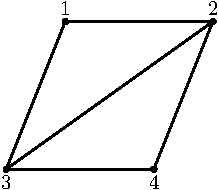
\includegraphics{gr-metapost-kim-1.pdf}
\hspace*{0.1truein}
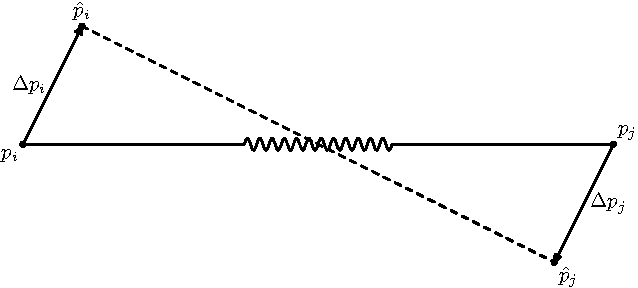
\includegraphics{gr-metapost-kim-2.pdf}

This is the |misc/gr-metapost-kim.mp| input file:
\MyI{misc/gr-metapost-kim.mp}

I typed, on Linux,\\
\hspace*{3\parindent}\Shell{mpost gr-metapost-kim}\\
\hspace*{3\parindent}\Shell{epstopdf gr-metapost-kim-1.mps;  epstopdf gr-metapost-kim-2.mps}\\
\hspace*{3\parindent}\Shell{mv -i gr-metapost-kim-1.pdf gr-metapost-kim-2.pdf ../graphics}\\
to run MetaPost and make |gr-metapost-kim-1.pdf|
and |gr-metapost-kim-2.pdf|,
and move them to the graphics subfolder.
\end{VerbatimOut}

\MyIO


\begin{VerbatimOut}{z.out}

\subsection{Tally example}
\label{ss:tally-example}

Whenever I use files with numbers in them I like to put leading zeros
in the names so they will be listed in order in the directory.

These 20 graphics (|gr-metapost-tally-01.pdf| through |gr-metapost-tally-20.pdf|)

\vspace*{6pt}

{%
  % Let * represent zero or more spaces!
  % Method 1: \def\g#1{ requires using \g*{10} for 10.
  %           Two shifted characters, { and } are needed.
  % Method 2: \def\g#1/{ requires using \g*10/ for 10.
  %           One unshifted character, / is needed.
  \def\g#1/{\includegraphics[scale=0.5]{gr-metapost-tally-#1.pdf}}%

  % Note that tabular* instead of tabular is used below.
  %   The {\textwidth} makes the total width of the table the width
  % of the printed area of the page.
  %   The @{\kern2\parindent} puts blank space the width of two
  % paragraph indents before the first column.
  %   The @{extracolsep{\fill}} adds \fill space between all subsequent
  % columns.
  %   The lll left justifies the next three columns.
  % after the column.
  %   The @{\kern2\parindent} puts blank space the width of two
  % paragraph indents before the first column.
  \begin{tabular*}{\textwidth}{@{\kern2\parindent}@{\extracolsep{\fill}}lll@{\kern2\parindent}}%
    \g 01/& \g 02/& \g 03/\\
    \g 04/& \g 05/& \g 06/\\
    \g 07/& \g 08/& \g 09/\\
    \g 10/& \g 11/& \g 12/\\
    \g 13/& \g 14/& \g 15/\\
    \g 16/& \g 17/& \g 18/\\
    \g 19/& \g 20/\\
  \end{tabular*}%
}
\noindent were produced by

\MyI{misc/gr-metapost-tally.mp}

\end{VerbatimOut}

\MyIO


\begin{VerbatimOut}{z.out}
\section{Python programming language}
\ix{Python programming language}

\lightgreen{Python can be set up to use \LaTeX\ fonts.}

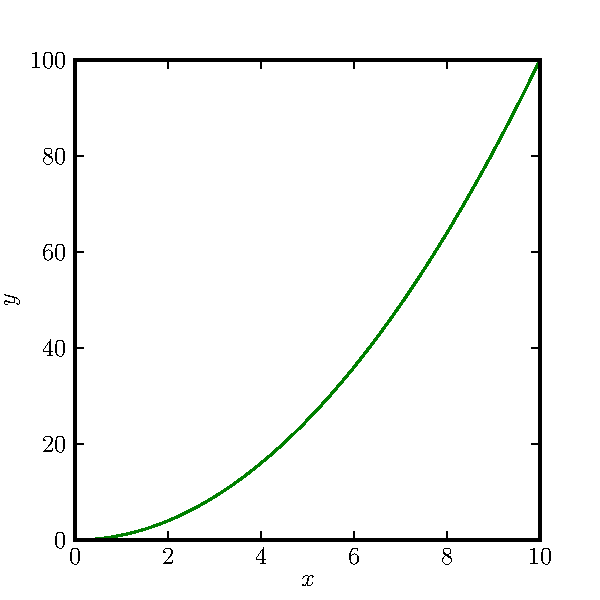
\includegraphics{gr-python2.pdf}

This is the |misc/gr-python2.py| input file:
\MyI{misc/gr-python2.py}

I typed, on Linux,
\Shell{./gr-python2.py}
in the |misc| subdirectory
to make the\\
|graphics/gr-python2.pdf| output file.
\end{VerbatimOut}

\MyIO



\begin{VerbatimOut}{z.out}

\section{R programming language}
\ix{R programming language}

\lightgreen{R can be set up to use \LaTeX\ fonts.}

% Created by tikzDevice version 0.6.2-92-0ad2792 on 2021-11-24 17:04:02
% !TEX encoding = UTF-8 Unicode
\begin{tikzpicture}[x=1pt,y=1pt]
\definecolor[named]{fillColor}{rgb}{1.00,1.00,1.00}
\path[use as bounding box,fill=fillColor,fill opacity=0.00] (0,0) rectangle (361.35,361.35);
\begin{scope}
\path[clip] ( 49.20, 61.20) rectangle (336.15,312.15);
\definecolor[named]{drawColor}{rgb}{0.00,0.00,0.00}

\path[draw=drawColor,line width= 0.4pt,line join=round,line cap=round] ( 59.83, 70.49) --
	( 62.48, 70.52) --
	( 65.14, 70.59) --
	( 67.80, 70.70) --
	( 70.46, 70.87) --
	( 73.11, 71.08) --
	( 75.77, 71.33) --
	( 78.43, 71.63) --
	( 81.08, 71.98) --
	( 83.74, 72.38) --
	( 86.40, 72.82) --
	( 89.05, 73.31) --
	( 91.71, 73.84) --
	( 94.37, 74.42) --
	( 97.03, 75.05) --
	( 99.68, 75.72) --
	(102.34, 76.44) --
	(105.00, 77.21) --
	(107.65, 78.02) --
	(110.31, 78.88) --
	(112.97, 79.79) --
	(115.62, 80.74) --
	(118.28, 81.74) --
	(120.94, 82.79) --
	(123.59, 83.88) --
	(126.25, 85.02) --
	(128.91, 86.20) --
	(131.57, 87.43) --
	(134.22, 88.71) --
	(136.88, 90.04) --
	(139.54, 91.41) --
	(142.19, 92.82) --
	(144.85, 94.29) --
	(147.51, 95.80) --
	(150.16, 97.36) --
	(152.82, 98.96) --
	(155.48,100.61) --
	(158.13,102.30) --
	(160.79,104.05) --
	(163.45,105.84) --
	(166.11,107.67) --
	(168.76,109.55) --
	(171.42,111.48) --
	(174.08,113.46) --
	(176.73,115.48) --
	(179.39,117.55) --
	(182.05,119.66) --
	(184.70,121.82) --
	(187.36,124.03) --
	(190.02,126.28) --
	(192.68,128.58) --
	(195.33,130.93) --
	(197.99,133.32) --
	(200.65,135.76) --
	(203.30,138.25) --
	(205.96,140.78) --
	(208.62,143.36) --
	(211.27,145.99) --
	(213.93,148.66) --
	(216.59,151.38) --
	(219.24,154.14) --
	(221.90,156.96) --
	(224.56,159.81) --
	(227.22,162.72) --
	(229.87,165.67) --
	(232.53,168.67) --
	(235.19,171.71) --
	(237.84,174.80) --
	(240.50,177.94) --
	(243.16,181.12) --
	(245.81,184.35) --
	(248.47,187.63) --
	(251.13,190.95) --
	(253.78,194.32) --
	(256.44,197.74) --
	(259.10,201.20) --
	(261.76,204.71) --
	(264.41,208.26) --
	(267.07,211.86) --
	(269.73,215.51) --
	(272.38,219.21) --
	(275.04,222.95) --
	(277.70,226.73) --
	(280.35,230.57) --
	(283.01,234.45) --
	(285.67,238.38) --
	(288.32,242.35) --
	(290.98,246.37) --
	(293.64,250.43) --
	(296.30,254.55) --
	(298.95,258.71) --
	(301.61,262.91) --
	(304.27,267.16) --
	(306.92,271.46) --
	(309.58,275.81) --
	(312.24,280.20) --
	(314.89,284.64) --
	(317.55,289.12) --
	(320.21,293.65) --
	(322.87,298.23) --
	(325.52,302.86);
\end{scope}
\begin{scope}
\path[clip] (  0.00,  0.00) rectangle (361.35,361.35);
\definecolor[named]{drawColor}{rgb}{0.00,0.00,0.00}

\path[draw=drawColor,line width= 0.4pt,line join=round,line cap=round] ( 59.83, 61.20) -- (325.52, 61.20);

\path[draw=drawColor,line width= 0.4pt,line join=round,line cap=round] ( 59.83, 61.20) -- ( 59.83, 55.20);

\path[draw=drawColor,line width= 0.4pt,line join=round,line cap=round] (112.97, 61.20) -- (112.97, 55.20);

\path[draw=drawColor,line width= 0.4pt,line join=round,line cap=round] (166.11, 61.20) -- (166.11, 55.20);

\path[draw=drawColor,line width= 0.4pt,line join=round,line cap=round] (219.24, 61.20) -- (219.24, 55.20);

\path[draw=drawColor,line width= 0.4pt,line join=round,line cap=round] (272.38, 61.20) -- (272.38, 55.20);

\path[draw=drawColor,line width= 0.4pt,line join=round,line cap=round] (325.52, 61.20) -- (325.52, 55.20);

\node[text=drawColor,anchor=base,inner sep=0pt, outer sep=0pt, scale=  1.00] at ( 59.83, 39.60) {0};

\node[text=drawColor,anchor=base,inner sep=0pt, outer sep=0pt, scale=  1.00] at (112.97, 39.60) {2};

\node[text=drawColor,anchor=base,inner sep=0pt, outer sep=0pt, scale=  1.00] at (166.11, 39.60) {4};

\node[text=drawColor,anchor=base,inner sep=0pt, outer sep=0pt, scale=  1.00] at (219.24, 39.60) {6};

\node[text=drawColor,anchor=base,inner sep=0pt, outer sep=0pt, scale=  1.00] at (272.38, 39.60) {8};

\node[text=drawColor,anchor=base,inner sep=0pt, outer sep=0pt, scale=  1.00] at (325.52, 39.60) {10};

\path[draw=drawColor,line width= 0.4pt,line join=round,line cap=round] ( 49.20, 70.49) -- ( 49.20,302.86);

\path[draw=drawColor,line width= 0.4pt,line join=round,line cap=round] ( 49.20, 70.49) -- ( 43.20, 70.49);

\path[draw=drawColor,line width= 0.4pt,line join=round,line cap=round] ( 49.20,116.97) -- ( 43.20,116.97);

\path[draw=drawColor,line width= 0.4pt,line join=round,line cap=round] ( 49.20,163.44) -- ( 43.20,163.44);

\path[draw=drawColor,line width= 0.4pt,line join=round,line cap=round] ( 49.20,209.91) -- ( 43.20,209.91);

\path[draw=drawColor,line width= 0.4pt,line join=round,line cap=round] ( 49.20,256.38) -- ( 43.20,256.38);

\path[draw=drawColor,line width= 0.4pt,line join=round,line cap=round] ( 49.20,302.86) -- ( 43.20,302.86);

\node[text=drawColor,rotate= 90.00,anchor=base,inner sep=0pt, outer sep=0pt, scale=  1.00] at ( 34.80, 70.49) {0};

\node[text=drawColor,rotate= 90.00,anchor=base,inner sep=0pt, outer sep=0pt, scale=  1.00] at ( 34.80,116.97) {20};

\node[text=drawColor,rotate= 90.00,anchor=base,inner sep=0pt, outer sep=0pt, scale=  1.00] at ( 34.80,163.44) {40};

\node[text=drawColor,rotate= 90.00,anchor=base,inner sep=0pt, outer sep=0pt, scale=  1.00] at ( 34.80,209.91) {60};

\node[text=drawColor,rotate= 90.00,anchor=base,inner sep=0pt, outer sep=0pt, scale=  1.00] at ( 34.80,256.38) {80};

\node[text=drawColor,rotate= 90.00,anchor=base,inner sep=0pt, outer sep=0pt, scale=  1.00] at ( 34.80,302.86) {100};

\path[draw=drawColor,line width= 0.4pt,line join=round,line cap=round] ( 49.20, 61.20) --
	(336.15, 61.20) --
	(336.15,312.15) --
	( 49.20,312.15) --
	( 49.20, 61.20);
\end{scope}
\begin{scope}
\path[clip] (  0.00,  0.00) rectangle (361.35,361.35);
\definecolor[named]{drawColor}{rgb}{0.00,0.00,0.00}

\node[text=drawColor,anchor=base,inner sep=0pt, outer sep=0pt, scale=  1.00] at (192.68, 15.60) {$x$};

\node[text=drawColor,rotate= 90.00,anchor=base,inner sep=0pt, outer sep=0pt, scale=  1.00] at ( 10.80,186.67) {$y$};
\end{scope}
\end{tikzpicture}


This is the |misc/gr-r.R| input file:
\MyI{misc/gr-r.R}

I typed, on Linux,
\Shell{R CMD BATCH gr-r}
in the |misc| subdirectory to make the |gr-r.tex| outfile file.
\end{VerbatimOut}

\MyIO


\begin{VerbatimOut}{z.out}

\section{\TikZLogo\ \LaTeX\ package}
\index{TikZ@\TikZLogo\ \LaTeX\ package}  
\todoindex{\TikZLogo\ \LaTeX\ package}

\lightgreen{\TikZLogo\ uses \LaTeX\ fonts.}
\end{VerbatimOut}

\MyIO


\begin{VerbatimOut}{z.out}

\subsection{Clock example}
\index{clock \TikZLogo\ example}
\todoindex{clock \TikZLogo\ example}
\end{VerbatimOut}

\MyIO


\begin{VerbatimOut}{z.out}

\index{TikZ@\TikZLogo}

\hbox to\textwidth{%
  \hfil
  % The idea for this clock was originally from a Google+ posting by Afamefuna ``Ferdy'' Ibeabuchia.
  \begin{tikzpicture}
    \def\CenterRadius{0.04cm}
    \def\InnerTickRadius{3.6cm}
    \def\OuterTickRadius{3.8cm}
    % Make \LR be an abbreviation for \LabelRadius so the
    % lines below will fit within the width of the page.
    \def\LabelRadius{4.5cm}      \let\LR=\LabelRadius
    \def\HourHandRadius{2.5cm}   \def\HourHandBase{0.3cm}
    \def\MinuteHandRadius{3cm}   \def\MinuteHandBase{0.4cm}
    \def\SecondHandRadius{3.5cm} \def\SecondHandBase{0.5cm}
    \def\DS{\displaystyle}
    \fill (0,0) circle (\CenterRadius);
    \foreach \i in {0,30,...,330}
    \draw (\i:\InnerTickRadius)--(\i:\OuterTickRadius);
    \node at (  0:\LR) {$\DS \qquad \sqrt9 + 9 - 9$};        %  3
    \node at ( 30:\LR) {$\DS \frac{9+9}9$};                  %  2
    \node at ( 60:\LR) {$\DS \frac{\sqrt9\sqrt9}9$};         %  1
    \node at ( 90:\LR) {$\DS 9 + \frac9{\sqrt9}$};           % 12
    \node at (120:\LR) {$\DS \frac{99}9$};                   % 11
    \node at (150:\LR) {$\DS 9 + \frac99$};                  % 10
    \node at (180:\LR) {$\DS \sqrt[\scriptstyle 9]{9^9}$};   %  9
    \node at (210:\LR) {$\DS 9 - \frac99$};                  %  8
    \node at (240:\LR) {$\DS 9 - \sqrt9 + \lceil.9\rceil$};  %  7
    \node at (270:\LR) {$\DS 9 - \frac9{\sqrt9}$};           %  6
    \node at (300:\LR) {$\DS \sqrt9\,! - \frac99$};          %  5
    \node at (330:\LR) {$\DS \sqrt9 + \frac99$};             %  4
    % In the following
    %   ABBREVIATION    DESCRIPTION
    %   deg             degrees
    %   min             minutes
    %   sec             seconds
    % for second hand:
    %   (9 sec/60 sec) * 360 deg = 54 deg;
    %   90 deg - 54 deg = 36 deg
    \draw[rotate around={36:(0,0)}]
      (-\SecondHandBase,\SecondHandBase) -- (\SecondHandRadius,0)
        -- (-\SecondHandBase,-\SecondHandBase) -- cycle;
    % for minute hand:
    %   (9 min/60 min) * 360 deg = 54 deg;
    %   90 deg - 54 deg = 36 deg
   \draw[rotate around={36:(0,0)}]
     (-\MinuteHandBase,\MinuteHandBase) -- (\MinuteHandRadius,0)
       -- (-\MinuteHandBase,-\MinuteHandBase) -- cycle;
    % for hour hand:
    %   (9 min * (60 sec/1 min)) + 9 sec) / 3600 sec
    %     = 549 sec / 3600 sec = 0.1525
    %   The hour hand is 0.1525 of the way from 9:00 to 10:00.
    %   Each hour is 30 degrees on the clock, so the hour hand
    %   position is
    %     30 deg * 0.1525 = 4.575 deg past 9:00
    %   180 deg - 4.575 deg = 175.425 deg
    \draw[rotate around={175.425:(0,0)}]
      (-\HourHandBase,\HourHandBase) -- (\HourHandRadius,0)
      -- (-\HourHandBase,-\HourHandBase) -- cycle;
  \end{tikzpicture}
  \hfil
}
\end{VerbatimOut}

\MyIO


\begin{VerbatimOut}{z.out}

\newpage

\subsection{counter example}
\label{ss:counter-example}
\index{counter \TikZLogo\ example}
\todoindex{counter \TikZLogo\ example}

\begin{tikzpicture}[scale=0.13]
  % Define points.
  \coordinate   (p11) at (  0, 78);
    \coordinate (p14) at ( 35, 78);
    \coordinate (p15) at ( 54, 78);
    \coordinate (p16) at ( 73, 78);
    \coordinate (p19) at (108, 78);
  \coordinate   (p24) at ( 35, 67);
    \coordinate (p26) at ( 73, 67);
  \coordinate   (p35) at ( 54, 63);
  \coordinate   (p44) at ( 35, 56);
    \coordinate (p46) at ( 73, 56);
  \coordinate   (p53) at ( 30, 48);
    \coordinate (p55) at ( 54, 48);
    \coordinate (p57) at ( 78, 48);
  \coordinate   (p69) at (108, 39);
  \coordinate   (p71) at (  0, 24);
    \coordinate (p72) at ( 15, 24);
    \coordinate (p73) at ( 30, 24);
    \coordinate (p75) at ( 54, 24);
    \coordinate (p77) at ( 78, 24);
    \coordinate (p78) at ( 93, 24);
    \coordinate (p79) at (108, 24);
  \coordinate   (p81) at (  0,  0);
    \coordinate (p83) at ( 30,  0);
    \coordinate (p85) at ( 54,  0);
    \coordinate (p87) at ( 78,  0);
    \coordinate (p89) at (108,  0);
  % Put "wall" above drawing.
  \draw (p15) node[above] {\large wall};
  % Plot outer edge.
  \draw (p81) -- (p11) -- (p19) -- (p89);
  % Plot inner edge.
  \draw (p83) -- (p53) -- (p57) -- (p87);
  % Color the counter. 
  \fill[blue!10] (p81) -- (p11) -- (p19) -- (p89) -- (p87) -- (p57) -- (p53) -- (p83) -- cycle;
  % Vertical measurement lines.
  \draw[dashed, arrows = {Stealth[inset=0pt, angle=30:8pt]-Stealth[inset=0pt, angle=30:8pt]}]
    (p14) -- (p44);
  \draw (p24) node[fill=blue!10] {$22''$};
  \draw[arrows = {Stealth[inset=0pt, angle=30:8pt]-Stealth[inset=0pt, angle=30:8pt]}] (p15) -- (p55);
  \draw (p35) node[fill=blue!10] {$30''$};
  \draw[dashed, arrows = {Stealth[inset=0pt, angle=30:8pt]-Stealth[inset=0pt, angle=30:8pt]}]
    (p16) -- (p46);
  \draw (p26) node[fill=blue!10] {$22''$};
  \draw[arrows = {Stealth[inset=0pt, angle=30:8pt]-Stealth[inset=0pt, angle=30:8pt]}] (p55) -- (p85);
  % Horizontal measurement lines.
  \draw[arrows = {Stealth[inset=0pt, angle=30:8pt]-Stealth[inset=0pt, angle=30:8pt]}] (p71) -- (p73);
  \draw (p72) node[fill=blue!10] {$30''$};
  \draw[arrows = {Stealth[inset=0pt, angle=30:8pt]-Stealth[inset=0pt, angle=30:8pt]}] (p73) -- (p77);
  \draw (p75) node[fill=white] {$48''$};
  \draw[arrows = {Stealth[inset=0pt, angle=30:8pt]-Stealth[inset=0pt, angle=30:8pt]}] (p77) -- (p79);
  \draw (p78) node[fill=blue!10] {$30''$};
  % Put "wall" to the right of drawing.
  \draw (p69) node[right] {\large wall};
\end{tikzpicture}
\end{VerbatimOut}

\MyIO


\begin{VerbatimOut}{z.out}

\subsection{Fourier transform example}
\label{ss:fourier-transform-example}
\index{Fourier transform \TikZLogo\ example}
\todoindex{Fourier transform \TikZLogo\ example}
  
The Fourier transform decomposes a function
into the frequencies that make it up.
The inverse Fourier transformation combines the contributions
of all the different frequencies to recover the original function.

(Mark Senn {\tt\char'074}mark@purdue.edu{\tt\char'076} wrote sales@aavos.be on 2021-09-03
to ask permission
to use
\href{https://aavos.eu/glossary/fourier-transform/}{Fourier transform}
as the starting point
for an example \TikZLogo\ figure.  
Dominique Demurie {\tt\char'074}sales@aavos.be{\tt\char'076} replied
on 2021-09-06 with
``I think it is not an original drawing from us either.
We had it for years on our website,
but I cannot remember where we got it from.
We don't mind you using it for a thesis.'')

% Run this with
%     pdflatex --shell-escape t
% That makes the t.table.* files.
%
% See
%     https://ctan.math.washington.edu/tex-archive/graphics/pgf/base/doc/pgfmanual.pdf
%     PAGE    TOPIC
%      655    decorations.text library to draw text 
%     1221    animations
%
% for text decorations, which includes text along a path information.
% Also see
%     https://tex.stackexchange.com/questions/427454/tikz-3dplot-and-rotation-of-coordinates
%     https://tex.stackexchange.com/questions/67573/tikz-shift-and-rotate-in-3d
%     http://tug.ctan.org/graphics/pgf/contrib/tikz-3dplot/tikz-3dplot_documentation.pdf
%     https://tex.stackexchange.com/questions/45848/rotate-node-text-and-use-relative-positioning-in-tikz
  
% was scale = 2
\begin{tikzpicture}[domain=0:6.283185, rotate around y=-55, scale=1]

  % total plot
  \begin{scope}[canvas is xy plane at z=0]
    \node[below=3pt] at (0,        -1) {0};
    \node[below=3pt] at (3.141593, -1) {$\pi$};
    \node[below=5pt] at (5.683185, -1) {$2\pi$};
    \draw[ultra thick,color=violet] plot[id=total,smooth] function{0.8*sin(x)+0.2*sin(8*x)};
    \draw[thin,color=black] (0,-1) -- (0,1) -- (6.283185,1) -- (6.283185,-1) -- cycle;
    \draw[thin,color=black] (0,0) -- (6.283185,0);
    \path[decorate,decoration={text along path,
% |\LARGE|
      text={Time Domain}}] (0.1,-2) -- (6.283185,-2); 
    % $s(t)$
  \end{scope}

  % tall plot
  \begin{scope}[canvas is xy plane at z=-1.5]
    \draw[dashed] (0,0.8) -- (6.283185,0.8);
    \draw[dashed] (0,-0.8) -- (6.283185,-0.8);
    \draw[thick,color=orange] plot[id=tall,smooth] function{0.8*sin(x)};
    \draw[thin,color=black] (0,-1) -- (0,1) -- (6.283185,1) -- (6.283185,-1) -- cycle;
    \draw[thin,color=black] (0,0) -- (6.283185,0);
  \end{scope}

  % short plot
  \begin{scope}[canvas is xy plane at z=-3.0]
    \draw[dashed] (0, 0.2) -- (6.283185,  0.2);
    \draw[dashed] (0,-0.2) -- (6.283185, -0.2);
    \draw[thick,color=green] plot[id=short,smooth] function{0.2*sin(2*x)};
    \draw[thin,color=black] (0,-1) -- (0,1) -- (6.283185,1) -- (6.283185,-1) -- cycle;
    \draw[thin,color=black] (0,0) -- (6.283185,0);
  \end{scope}

  % frequency plot
  \begin{scope}[canvas is zy plane at x=6.283185]
    \node[below=3pt] at ( 0.0,-1) {0};
    \node[below=3pt] at (-1.5,-1) {1};
    \node[below=3pt] at (-3.0,-1) {2};
    \draw[thin,color=black] (0,-1.0) -- (-3.0,-1.0);  \node[above=-9pt] at (-3.3,-1.0) {$-1.0$};
    \draw[thin,color=black] (0,-0.8) -- (-3.0,-0.8);  \node[above=-9pt] at (-3.3,-0.8) {$-0.8$};
    \draw[thin,color=black] (0,-0.2) -- (-3.0,-0.2);  \node[above=-9pt] at (-3.3,-0.2) {$-0.2$};
    \draw[thin,color=black] (0, 0.0) -- (-3.0, 0.0);  \node[above=-9pt] at (-3.3, 0.0) {$\phantom-0.0$};
    \draw[thin,color=black] (0, 0.2) -- (-3.0, 0.2);  \node[above=-9pt] at (-3.3, 0.2) {$\phantom-0.2$};
    \draw[thin,color=black] (0, 0.8) -- (-3.0, 0.8);  \node[above=-9pt] at (-3.3, 0.8) {$\phantom-0.8$};
    \draw[thin,color=black] (0, 1.0) -- (-3.0, 1.0);  \node[above=-9pt] at (-3.3, 1.0) {$\phantom-1.0$};
    \draw[line width=6pt,color=red] (-1.5,0) -- (-1.5,0.8);
    \draw[line width=6pt,color=red] (-3.0,0) -- (-3.0,0.2);
    \path[decorate,decoration={text along path,
% |\LARGE|
      text={Frequency Domain}}] (-0.8,-1.6) -- (-3.0,-1.6); 
    % $S(\omega)$
  \end{scope}

  %% legend
  %% Wolfram Language code:
  %%     In[1]:= ry[theta_] :=
  %%     {
  %%         {Cos[theta Degree],  0, Sin[theta Degree]},
  %%         {0,                  1, 0},
  %%         {-Sin[theta Degree], 0, Cos[theta Degree]}
  %%     }
  %%
  %%     ry[55] . {Pi, 0.7, -3.5}
  %%     # Out[] = {-1.06509, 0.7, -4.58096}
  %%     ry[55] . {(3/4)Pi, 0.7, -3.5}
  %%     # Out[] = {-1.51557, 0.7, -3.9376}

  \draw[ultra thick,color=violet] (2.45782, 1.7, -4.33538) -- (1.06509, 0.7, -4.58096);
    \node[right] at                                           (1.06509, 0.7, -4.58096)
                                                                {$0.8\sin x + 0.2\sin 2x$};
  \draw[ultra thick,color=orange] (0.08509, 0.4, -4.58096) -- (1.06509, 0.4, -4.58096);
    \node[right] at                                           (1.06509, 0.4, -4.58096) {$0.8\sin x$};
  \draw[ultra thick,color=green]  (0.08509, 0.1, -4.58096) -- (1.06509, 0.1, -4.58096);
    \node[right] at                                           (1.06509, 0.1, -4.58096) {$0.2\sin 2x$};
\end{tikzpicture}
\end{VerbatimOut}

\MyIO


\begin{VerbatimOut}{z.out}

\subsection{Glider example}
\ix{Hirzel, Alex}
\index{glider \TikZLogo\ example}
\todoindex{glider \TikZLogo\ example}

The glider
is a pattern from the Game of Life,
and it's used as an emblem representing the hacker community.

\begin{tikzpicture}[thick]
  \draw (0,0) grid (3,3);
  \foreach \c in {(0,0), (1,0), (2,0), (2,1), (1,2)}
    \fill \c + (0.5,0.5) circle (0.42);
\end{tikzpicture}
\end{VerbatimOut}

\MyIO


\begin{VerbatimOut}{z.out}

% If you use the silence package change
\subsection{Sum of 1 to \(n\) example}
% to
%     \subsection{Sum of 1 to $n$ example}
% to avoid having the silence package apparently go into an infinite
% loop.
% \ix{sum of 1 to \(n\)}

What is the sum of \(1 \text{ to } n\)?

Pair the numbers 1 and 10, 2 and 9, \ldots\,:

\hbox to\textwidth{%
  \hss  % horizontal stretch or shrink as needed
  \vspace*{0.25in}
  % Curves leave a node at a 30 degree angle
  % and enter a node at a 150 degree angle.
  \begin{tikzpicture}[out=30,in=150]
    \node at  (1,0)  {1};
    \node at  (2,0)  {2};
    \node at  (3,0)  {3};
    \node at  (4,0)  {4};
    \node at  (5,0)  {5};
    \node at  (6,0)  {6};
    \node at  (7,0)  {7};
    \node at  (8,0)  {8};
    \node at  (9,0)  {9};
    \node at (10,0) {10};
    \draw (1.2, 0.2) to (9.8, 0.2)
          (2.2, 0.2) to (8.8, 0.2)
          (3.2, 0.2) to (7.8, 0.2)
          (4.2, 0.2) to (6.8, 0.2)
          (5.2, 0.2) to (5.8, 0.2);
  \end{tikzpicture}%
  \hss
}

So
\begin{align}
  % Since i is interpreted as a constant and is an upright font by default
  % I'm using {\mit i} so it is in a math italic font.
  \sum_1^n &= \text{how many pairs of numbers}
    \times \text{the sum of each pair}\nonumber\\
  &= \left(\frac n 2\right) (n+1)\nonumber\\
  &= \frac {n (n+1)} 2
\end{align}
This also works if \(n\) is an odd number.
(The famous mathematician Gauss reportedly added
the numbers~1--100 quickly in~1784
but the best reference I could find
\cite[page 3--4]{waltershausen1856}                                             
did not state which method he used.)
\end{VerbatimOut}

\MyIO


\begin{VerbatimOut}{z.out}

\newpage

\subsection{Tree example}
\ix{???, ???}
\index{tree \TikZLogo\ example}
\todoindex{tree \TikZLogo\ example}

{
  \def\f#1#2{$\displaystyle\frac #1#2$}
  \begin{tikzpicture}%
  [%
    level 1/.style={sibling distance=60mm},
    level 2/.style={sibling distance=30mm},
    level 3/.style={sibling distance=15mm}
  ]
    \node {\f 11}
      child {node {$\displaystyle\frac 12$}
        child {node {\f 13}
          child {node {\f 14}}
          child {node {\f 48}}
        }
        child {node {\f 32}
          child {node {\f 35}}
          child {node {\f 52}}
        }
      }
      child {node {\f 21}
        child {node {\f 23}
          child {node {\f 25}}
          child {node {\f 53}}
        }
        child {node {\f 31}
          child {node {\f 34}}
          child {node {\f 41}}
        }
      };
  \end{tikzpicture}    

\vspace*{4pt}
The node with value \f nd\\[2pt]
\indent\hspace*{4\parindent}
\begin{tabular}{@{}llll@{}}
  \bfseries with additional conditions& \bfseries has& \bfseries with value\\
  \noalign{\vspace{2pt}}
  (none)&                     left child&     \f n{{n+d}}\\
  \noalign{\vspace{12pt}}
  (none)&                     right child&    \f {{n+d}}d\\
  \noalign{\vspace{12pt}}
  $n<d$&                      parent&         \f n{{d-n}}\\
  \noalign{\vspace{12pt}}
  $n=d$&                      no parent&      (not applicable)\\
  \noalign{\vspace{12pt}}
  $n>d$&                      parent&         \f {{n-d}}d\\
\end{tabular}
}
\end{VerbatimOut}

\MyIO

\begin{VerbatimOut}{z.out}


\subsection{Yin and yang example}

This Yin and yang example was done by Thomas G. Kristensen \cite{kristensen}.
This is the ``traditional Taijitu symbol from Chinese philosophy''.
\ix{Kristensen, Thomas G.//Taijitu symbol//Yin and yang symbol}

\index{TikZ@\TikZLogo}  
\begin{tikzpicture}
  % Yin and yang
  % Author: Thomas G. Kristensen
  
  % color one half of a unit circle                                              
  \begin{scope}
    \clip (0,0) circle (1cm);
    \fill[black] (0cm,1cm) rectangle (-1cm, -1cm);
  \end{scope}

  % fill heads                                                                   
  \fill[black] (0,0.5) circle (0.5cm);
  \fill[white] (0,-0.5) circle (0.5cm);

  % fill eyes                                                                    
  \fill[white] (0,0.5) circle (0.1cm);
  \fill[black] (0,-0.5) circle (0.1cm);

  % outer line                                                                   
  \draw (0,0) circle (1cm);

\end{tikzpicture}
\end{VerbatimOut}

\MyIO


\begin{VerbatimOut}{z.out}

\section{Wolfram Language (Mathematica uses this)}
\ix{Mathematica}
\ix{Wolfram Language}

\lightgreen{Wolfram Language can be set up to use \LaTeX\ fonts.}

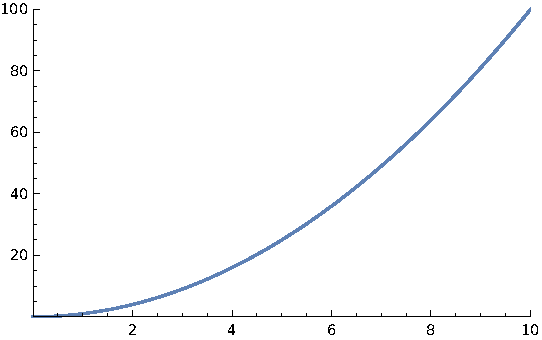
\includegraphics{gr-mathematica.pdf}

This is the |misc/gr-mathematica.ma| input file
\MyI{misc/gr-mathematica.ma}

I typed, on Linux,
\Shell{math < gr-mathematica.ma}
in the |misc| subdirectory
to make the |graphics/gr-mathematica.pdf| output file.
\end{VerbatimOut}

\MyIO


  % How to debug LaTeX Problems.
  \ProvidesFile{ap-how-to-debug-latex-problems}[2023-08-30 How to Debug LaTeX Problems]

\begin{VerbatimOut}{z.out}
\chapter
  [HOW TO DEBUG LATEX PROBLEMS]%
  {HOW TO DEBUG \LaTeX\ PROBLEMS}
\ix{debugging \LaTeX//How to Debug \LaTeXLogo\ Problems appendix}
\end{VerbatimOut}

\MyIO


\begin{VerbatimOut}{z.out}

Add more content here.
\todoerror{add more content here}
\end{VerbatimOut}

\MyIO


\ProvidesFile{ap-debugging.tex}[2023-06-16 debugging appendix]


In \LuaLaTeXLogo\ error messages,
the |l| in,
for example,
|l.987| means |line|.
|l.987| means |line 987|.

|! Undefined control sequence.|
|l.|\emph{line\_number} |\|\emph{command}|}|

The
\emph{command}
on
\emph{line\_number}
of the current file does not exist.
It may be misspelled.

\endinput

\begin{environment}
mispelled

too many }

use \begin{tabular} instead of \halign

\alpha
not in m'th mode

\show \var

\showthe \dimension


compile input often

providing ``too many'' causes extra arguementl to be printed

Don't use the |unravel| package for debugging.
It can cause more problems than it solves.

Use minimum working examples.


\begin{VerbatimOut}{z.out}
\chapter{DEBUGGING}
\ix{debugging//Debugging appendix}

\MyIO

Type 'R' to run LaTeX without showing errors.

\linenumbers
https://www.ametsoc.org/index.cfm/ams/publications/author-information/latex-author-info/preparing-a-latex-manuscript-for-submission/

Remove all files ending with |.aux|.
Those are temporary files
and wil be remade automatically by LaTeX.


\includeonly
\endinput   (can only do at level 0)
comment out with %

\begin{comment} \ldots\ \end{comment}
https://ctan.math.illinois.edu/macros/latex/contrib/comment/writeup.pdf

\end{document}



when you aren't in a text math (\(...\) or $...$ but I recommend \(...\))




Just want to make sure you know about the following:
after you recompile your document click on the icon to the
immediate right to show any errors.

There aren't any errors that have to do with your question.

A float is a table or a figure.  \hbox is a horizontal box.
There are 72.27 point (pt) per inch.

Putting \, (backslash comma) in math mode gives a tiny
bit of horizontal space.  You may want to put that before
"erfc".

You're right.  There is a problem.  I'll look at it with
fresh eyes this weekend.

I made a copy of the document and am making small changes to
it but it fails to compile,  (I thought making a copy of
it would not affect you.)  I'm confused.




\left   \right
\[    \]
\(   \)
{   }
\begin{whatever}   \end{whatever}


special characters:
# $ % & ~ _ ^ \ { }


don't use &#<digit><digit><digit><digut>& to try and get Unicode fonts in LaTeX

PurdueThesis does not support the inputenc package.  Use, for example, $beta$
for beta.
\let\savedbeta=\beta
beta = beta or $\savedbeta$

% in bibliography files


\qrmtz
can't find control sequence
it's either misspelled? ir your file or you didn't include a package that defined it

use formatting that will help you
  indenting

use tools that will help you


use Google

http://crab.rutgers.edu/~karel/latex/class4/class4.html
http://crab.rutgers.edu/~karel/latex/class5/class5.html
http://crab.rutgers.edu/~karel/latex/class6/class6.html





Michelle Krummel has a good Errors and Debugging tutorial.
See LaTeX Tutorial 7 below.  In case you're interested in
her other LaTeX tutorials they are in the table also.

NAME   DATE   LENGTH
LaTeX Tutorial 1 - Creating a LaTeX Document&
LaTeX Tutorial 2 - Common Mathematical Notation&
LaTeX Tutorial 3 - Brackets, Tables, and Arrays&
LaTeX Tutorial 4 - Creating Lists&
LaTeX Tutorial 5 - Text and Document Formatting&
LaTeX Tutorial 6: Packages, Macros and Graphics&
LaTeX Tutorial 7: Errors and Debugging&
LaTeX Tutorial 8: TeXmaker and Overleaf Tips&
LaTeX Tutorial 9 - Calculus Notation&
LaTeX Tutorial 10: How to Format a Math Paper&
LaTeX Tutorial 11: Beamer Slide Presentation&

@online{krummel?,
  author  = {Michelle Krummel},
  date    = {2020-07-08},
  note    = {35 minutes long},
  title   = {LaTeX Tutorial 1 - Creating a LaTeX Document},
  url     = {https://www.youtube.com/watch?v=0ivLZh9xK1Q},
  urldate = {2022-04-15},
}

@online{krummel?,
  author  = {Michelle Krummel},
  date    = {2020-07-27},
  note    = {36 minutes long},
  title   = {LaTeX Tutorial 2 - Common Mathematical Notation},
  url     = {https://www.youtube.com/watch?v=bCumVPGR4ts},
  urldate = {2022-04-15},
}

@online{krummel?,
  author  = {Michelle Krummel},
  date    = {2020-07-27},
  note    = {42 minutes long},
  title   = {LaTeX Tutorial 3 - Brackets, Tables, and Arrays},
  url     = {https://www.youtube.com/watch?v=kefvRACdXHs},
  urldate = {2022-04-15},
}

@online{krummel?,
  author  = {Michelle Krummel},
  date    = {2020-07-27},
  note    = {12 minutes long},
  title   = {LaTeX Tutorial 4 - Creating Lists},
  url     = {https://www.youtube.com/watch?v=dZitO3IJTys},
  urldate = {2022-04-15},
}

@online{krummel?,
  author  = {Michelle Krummel},
  date    = {2020-07-27},
  note    = {23 minutes long},
  title   = {LaTeX Tutorial 5 - Text and Document Formatting},
  url     = {https://www.youtube.com/watch?v=3KvsemMjHPU},
  urldate = {2022-04-15},
}

@online{krummel?,
  author  = {Michelle Krummel},
  date    = {2020-08-23},
  note    = {30 minutes},
  title   = {LaTeX Tutorial 6: Packages, Macros and Graphics},
  url     = {https://www.youtube.com/watch?v=L7WzLrzU2Ec},
  urldate = {2022-04-15},
}

@online{krummel?,
  author  = {Michelle Krummel
  date    = {2020-08-25},
  note    = {23 minutes long},
  title   = {LaTeX Tutorial 7: Errors and Debugging},
  url     = {https://www.youtube.com/watch?v=bYoTJc81-qk},
  urldate = {2022-04-15},
}
pp
@online{krummel?,
  author  = {Michelle Krummel},
  date    = {2020-08-25},
  note    = {41 minutes long},
  title   = {LaTeX Tutorial 8: TeXmaker and Overleaf Tips},
  url     = {https://www.youtube.com/watch?v=DzwoiIxrihA},
  urldate = {2022-04-15},
}

@online{krummel?,
  author  = {Michelle Krummel},
  date    = {2015-05-03},
  note    = {29 minutes long},
  title   = {LaTeX Tutorial 9 - Calculus Notation},
  url     = {https://www.youtube.com/watch?v=eDeRsE-NTb4},
  urldate = {2022-04-15},
}

@online{krummel?,
  author  = {Michelle Krummel},
  date    = {2016-10-03},
  note    = {25 minutes long},
  title   = {LaTeX Tutorial 10: How to Format a Math Paper},
  url     = {https://www.youtube.com/watch?v=FcVP3gGUtGI},
  urldate = {2022-04-15},
}

@online{krummel?,
  author  = {Michelle Krummel,
  date    = {2017-02-17},
  note    = {47 minutes long},
  tittle  = {LaTeX Tutorial 11: Beamer Slide Presentation},
  url     = {https://www.youtube.com/watch?v=0fsWGg81RwU},
  urldate = {2022-04-15},
}

I like powerdot better
Hendri Adriaens
The powerdot class
https://ctan.org/pkg/powerdot
2021/05/19
version = {1.7},
urldate = {2022-04-15}


  % Ignore these references.
  \ProvidesFile{ap-ignore-these-references.tex}[2023-03-20 ignore these references appendix]

\begin{VerbatimOut}{z.out}
\chapter{IGNORE THESE REFERENCES---THEY ARE WRONG}
\end{VerbatimOut}

\MyIO


\begin{VerbatimOut}{z.out}

You may have seen these references on the web.
Ignore them---they're wrong.
\end{VerbatimOut}

\MyIO


\begin{VerbatimOut}{z.out}

\noindent
\textbf{A Manual for the Preparation of [Purdue] Graduate Theses}
\cite{thesis2017}

\begin{quote}
  Parts of this are out of date.

  Thesis Help \(<\)thesishelp@purdue.edu\(>\) wrote on March 20, 2023:
  \begin{quote}
    Please look for current information on the
    \citetitle{thesisanddissertationofficeb}
    web page
    \cite{thesisanddissertationofficeb}.
  \end{quote}
\end{quote}
\end{VerbatimOut}

\MyIO


\begin{VerbatimOut}{z.out}

\noindent
\textbf{Purdue Online Writing Lab, IEEE Reference List}
\cite{owl}
  
\begin{quote}
  The IEEE
  (The world's largest technical professional organization
  for the advancement
  of technology)
  has changed their references format from,
  for example,
  
  \noindent
  \begin{tabular}{@{}ll@{}}
  \noalign{\vspace*{6pt}}
    [1]& W. K. Chen, Linear Networks and Systems. Belmont, CA: Wadsworth Press,\\
    \multispan{2}{2003.\hfil}\\
  \noalign{\vspace*{6pt}}
  \noalign{\noindent to}
  \noalign{\vspace*{6pt}}
    [1]& W. K. Chen, Linear Networks and Systems. Belmont, CA: Wadsworth Press,\\
    & 2003.\hfil\\
  \noalign{\vspace*{6pt}}
  \end{tabular}
  See
  \cite[page~2]{ieeedataport}.
\end{quote}
\end{VerbatimOut}

\MyIO


% BL  @online{owl,
% BT  @misc{owl,
%     author  = {Purdue Online Writing Lab},
%     title   = {IEEE Reference List},
%     url     = {https://owl.purdue.edu/owl/research_and_citation/ieee_style/reference_list.html},
% BL  urldate = {2022-03-17},
% }
% 
% BL  @online{ieeedataport,
% BT  @misc{ieeedataport,
%     author  = {IEEEDataPort},
%     title   = {How too Cite References: IEEE Documentation Style},
%     url     = {https://ieee-dataport.org/sites/default/files/analysis/27/IEEE%20Citation%20Guidelines.pdf},
% BL  urldate = {2022-03-17},
% }  


  % Logos.
  \ProvidesFile{ap-logos.tex}[2025-01-16 logos appendix]

\begin{VerbatimOut}{z.out}
\chapter{LOGOS}

These logos are defined in |pa-logos.sty|:

\begin{tabular}{@{}lll@{}}
  \toprule
  \bfseries Input& \bfseries Output& \bfseries Used In\\
  \midrule
  % From thesis.tex
  %     \newcommand{\tabularspace}{\noalign{\vspace*{2pt}}}
  % \tabularspace
  |\AMSmathLogo|& \AMSmathLogo\\[2pt]
  |\BibLaTeXLogo|& \BibLaTeXLogo\\[2pt]
  |\BiberLogo|& \BiberLogo\\[2pt]
  |\CalligraphicAMSLaTeXLogo|& \CalligraphicAMSLaTeXLogo\\[2pt]
  |\CircuiTikZLogo|& \CircuiTikZLogo\\[2pt]
  |\CTANLogo|& \CTANLogo\\[2pt]
  |\LaTeXLogo|& \LaTeXLogo\\[2pt]
  |\LuaLaTeXLogo|& \LuaLaTeXLogo\\[2pt]
  |\METAFONTLogo|& \METAFONTLogo\\[2pt]
  |\METAPOSTLogo|& \METAPOSTLogo& \cite{hobby2024}\\[2pt]
  |\MetaPostLogo|& \MetaPostLogo& \cite{hobby2024} and everywhere else I checked\\[2pt]
  |\NonCalligraphicAMSLaTeXLogo|& \NonCalligraphicAMSLaTeXLogo\\[2pt]
  |\PurdueThesisLogo|& \PurdueThesisLogo\\[2pt]
  |\PuThLogo|& \PuThLogo\\[2pt]
  |\siunitxLogo|& \siunitxLogo\\[2pt]
  |\TeXLogo|& \TeXLogo\\[2pt]
  |\TeXLiveLogo|& \TeXLiveLogo\\[2pt]
  |\TikZLogo|& \TikZLogo\\[2pt]
  |\TEXUsersGroupLogo|& \TeXUsersGroupLogo\\[2pt]
  |\TUGboatLogo|& \TUGboatLogo\\[2pt]
  \bottomrule
\end{tabular}
\end{VerbatimOut}

\MyIO


  % Numbers and Units.
  \ProvidesFile{ap-numbers-and-units.tex}[2025-01-14 numbers and units appendix]

%  Primary sources:
%      See https://www.bipm.org/utils/common/pdf/si-brochure/SI-Brochure-9-EN.pdf.
%      See https://www.nist.gov/pml/special-publication-811/nist-guide-si-chapter-4-two-classes-si-units-and-si-prefixes.
%
%  Notes:
%      See https://www.iso.org/standard/60241.html.

% Historic Vote Ties Kilogram and Other Units to Natural Constants
% NIST
% https://www.nist.gov/news-events/news/2018/11/historic-vote-ties-kilogram-and-other-units-natural-constants
% created 2018-11-16
% updated 2018-12-21
% last retrieved 2018-12-22

% https://www.bipm.org/utils/common/pdf/CGPM-2018/26th-CGPM-Resolutions.pdf
% Resolutions adopted
% 26^e CGPM
% Versailes
% 13--16 November 2018
% last retrieved 2018-12-30


\begin{VerbatimOut}{z.out}
\chapter{NUMBERS AND UNITS}
\end{VerbatimOut}

\MyIO


\begin{VerbatimOut}{z.out}

Note to self: scientific prefixes, scientific suffixes, tables.

The \PurdueThesisLogo\ documentclass
uses the siunitx \cite{wright2024} package
with some extra definitions in the puthesis.cls file
to do numbers and units.
\end{VerbatimOut}

\MyIO


\begin{VerbatimOut}{z.out}

\section{Number Examples}
\end{VerbatimOut}

\MyIO


\begin{VerbatimOut}{z.out}
\noindent\begin{tabular}{@{}lll@{}}
  \bfseries Input& \bfseries Output& \bfseries Comment\\
  \tabularspace
  \verb+\num{-0.12345}+& \num{-0.12345}& note the small space after the ``3''\\
  \verb+\num{-0.1234}+&
    \num{-0.1234}&
    note no space between the ``3'' and ``4''\\
  \verb+\num{-.123}+& \num{-.123}& the ``0.'' is inserted automatically\\
  \verb+\num{123}+& \num{123}\\
  \verb+\num{1234}+& \num{1234}\\
  \verb+\num{12345}+& \num{12345}& note the small space after the ``2''\\
  \verb+\num{2e4}+& \num{2e4}\\
  \verb+\num{e5}+& \num{e5}\\
  \verb+\num{2.34567e6}+&
    \num{2.34567e6}&
    note the small space after the ``5''\\
\end{tabular}
\end{VerbatimOut}

\MyIO


\begin{VerbatimOut}{z.out}

\section{Unit Examples}
\end{VerbatimOut}

\MyIO


\begin{VerbatimOut}{z.out}

See page~\pageref{se:Complete-List-of-Units}
for the complete list
of units defined by \PurdueThesisLogo.

\noindent\begin{tabular}{@{}lll@{}}
  \bfseries Input& \bfseries Output& \bfseries Comment\\
  \tabularspace
  \verb+\si{\kg}+& \si{\kg}& kilogram\\
  \verb+\si{\m}+& \si{\m}& meter\\
  \verb+\si{\kg\per\m\squared}+&
    \si{\kg\per\m\squared}&
    \(= \si{\kg}/\si{\m\squared}\)\\
\end{tabular}
\end{VerbatimOut}

\MyIO


\begin{VerbatimOut}{z.out}

\section{Combined Number and Unit Examples}
\end{VerbatimOut}

\MyIO


\begin{VerbatimOut}{z.out}
\begin{tabular}{@{}lll@{}}
  \bfseries Input& \bfseries Output& \bfseries Comment\\
  \tabularspace
  \verb+\SI{12}{\kg}+& \SI{12}{\kg}& 12 kilograms\\
  \verb+\SI{34}{\m}+&  \SI{34}{\m}& 34 meters\\
  % The next input line is too wide for the margins
  % so I'm splitting it into pieces.
  \verb+\SI{4.5e3}{\kg\per\m\squared}+&
    \SI{4.5e3}{\kg\per\m\squared}&
    \(= \num{4.5e3}\,\si{\kg}/\si{\m\squared}\)\\
\end{tabular}
\end{VerbatimOut}

\MyIO


\begin{VerbatimOut}{z.out}

How many seconds are in a non-leap year that does not have any leap seconds?
% I tried several things and couold not get \cancel to work with \per.
% Mark Senn    2019-12-29
\begin{align*}
           \frac{\SI{365}{\cancel\d}}{\si{\y}}
    \times \frac{\SI{24}{\cancel\h}}{\si{\cancel\d}}
    \times \frac{\SI{60}{\cancel\min}}{\si{\cancel\h}}         
    \times \frac{\SI{60}{\s}}{\si{\cancel\min}}         
    % From http://www.emerson.emory.edu/services/latex/latex_119.html
    %     Spacing in Math Mode
    %     In a math environment, LaTeX ignores the spaces you type
    %     and puts in the spacing that it thinks is best. LaTeX formats
    %     mathematics the way it's done in mathematics texts. If you
    %     want different spacing, LaTeX provides the following four
    %     commands for use in math mode:
    %         \; - a thick space
    %         \: - a medium space
    %         \, - a thin space
    %         \! - a negative thin space
    & = \num{31536000}\;\frac{\si{\s}}{\si{\y}}\\
    & = \SI{31536000}{\s\per\y}\\
    & \approx \SI{3e7}{\s\per\y}\\
    & \approx \text{30 million\,}\si{\s\per\y}\\
\end{align*}
\end{VerbatimOut}

\MyIO


\begin{VerbatimOut}{z.out}

\section{Binary Prefixes}
\end{VerbatimOut}

\MyIO


\begin{VerbatimOut}{z.out}

The
|\kibi|\ldots|\yobi|
commands are defined immediately after the
|\usepackage{siunitx}|
command in the PurdueThesis.cls file.
\end{VerbatimOut}

\MyIO


\begin{VerbatimOut}{z.out}

\newcolumntype{m}{>{$}r<{$}}  % math mode version of "r" column type
\renewcommand{\t}[4]{\(2^{#1}\) bytes is a #2, \(10^{#3}\) bytes is a #4}
\begin{tabular}{@{}mllll@{}}
  \multicolumn{1}{l}{\bfseries Power}&
    \bfseries Prefix&
    \bfseries Symbol&
    \bfseries Command&
    \bfseries Comment\\
  \tabularspace
  10& kibi& \unit{\kibi\nounit}& \verb+\si{\kibi}+& \t{10}{KB}{3}{KiB}\\
  20& mebi& \unit{\mebi\nounit}& \verb+\si{\mebi}+& \t{20}{MB}{6}{MiB}\\
  30& gibi& \unit{\gibi\nounit}& \verb+\si{\gibi}+& \t{30}{GB}{9}{GiB}\\
  40& tebi& \unit{\tebi\nounit}& \verb+\si{\tebi}+& \t{40}{TB}{12}{TiB}\\
  50& pebi& \unit{\pebi\nounit}& \verb+\si{\pebi}+& \t{50}{PB}{15}{PiB}\\
  60& exbi& \unit{\exbi\nounit}& \verb+\si{\exbi}+& \t{60}{EB}{18}{EiB}\\
  70& zebi& \unit{\zebi\nounit}& \verb+\si{\zebi}+& \t{70}{ZB}{21}{ZiB}\\
  80& yobi& \unit{\yobi\nounit}& \verb+\si{\yobi}+& \t{80}{YB}{24}{YiB}\\
\end{tabular}
\end{VerbatimOut}

\MyIO


\begin{VerbatimOut}{z.out}

\section{Decimal Prefixes}
\end{VerbatimOut}

\MyIO

\begin{VerbatimOut}{z.out}

\newcolumntype{m}{>{$}r<{$}}  % math mode version of "r" column type
\begin{tabular}{@{}mllll@{}}
  \multicolumn{1}{l}{\bfseries Power}&
    \bfseries Prefix&
    \bfseries Symbol&
    \bfseries Command&
    \bfseries Comment\\
  \tabularspace
  -30& quecto& \unit{\quecto\nounit}& \verb+\si{\quecto}+\\
  -27& ronto&  \unit{\ronto\nounit}&  \verb+\si{\quecto}+\\
  -24& yocto&  \unit{\yocto\nounit}&  \verb+\si{\yocto}+\\
  -21& zepto&  \unit{\zepto\nounit}&  \verb+\si{\zepto}+\\
  -18& atto&   \unit{\atto\nounit}&   \verb+\si{\atto}+\\
  -15& femto&  \unit{\femto\nounit}&  \verb+\si{\femto}+\\
  -12& pico&   \unit{\pico\nounit}&   \verb+\si{\pico}+\\
   -9& nano&   \unit{\nano\nounit}&   \verb+\si{\nano}+\\
   -6& micro&  \unit{\micro\nounit}&  \verb+\si{\micro}+\\
   -3& milli&  \unit{\milli\nounit}&  \verb+\si{\milla}+\\
   -2& centi&  \unit{\centi\nounit}&  \verb+\si{\centi}+\\
   -1& deci&   \unit{\deci\nounit}&   \verb+\si{\deci}+\\
    1& deca&   \unit{\deca\nounit}&   \verb+\si{\deca}+\\
    1& deka&   \unit{\deka\nounit}&   \verb+\si{\deka}+& same as \verb+\si{\deca}+\\
    2& hecto&  \unit{\hecto\nounit}&  \verb+\si{\hecto}+\\
    3& kilo&   \unit{\kilo\nounit}&   \verb+\si{\kilo}+\\
    6& mega&   \unit{\mega\nounit}&   \verb+\si{\mega}+\\
    9& giga&   \unit{\giga\nounit}&   \verb+\si{\giga}+\\
   12& tera&   \unit{\tera\nounit}&   \verb+\si{\tera}+\\
   15& peta&   \unit{\peta\nounit}&   \verb+\si{\peta}+\\
   18& exa&    \unit{\exa\nounit}&    \verb+\si{\exa}+\\
   21& zetta&  \unit{\zetta\nounit}&  \verb+\si{\zetta}+\\
   24& yotta&  \unit{\yotta\nounit}&  \verb+\si{\yotta}+\\
   27& ronna&  \unit{\ronna\nounit}&  \verb+\si{\ronna}+\\
   30& quetta& \unit{\quetta\nounit}& \verb+\si{\quetta}+\\
\end{tabular}
\end{VerbatimOut}

\MyIO


\begin{VerbatimOut}{z.out}

\section{SI Units}
\end{VerbatimOut}

\MyIO


\begin{VerbatimOut}{z.out}

The International System of Units
(SI)
% !!! Doing
% !!!     \include{tipa}
% !!! in thesis.tex so \textprimstress works
% !!! apparently causes problems with math commands.
% !!! Figure out why the following doesn't work later.
% (%
%   SI,
%   abbreviated from the French Syst\`eme International
%   (d\textprimstress unit\'es)%
% )
is the modern form of the metric system.
There are seven SI base units:

\hspace{40pt}
\begin{tabular}{@{}lll@{}}
  \tabularspace
  \bfseries Name& \bfseries Unit Of&         \bfseries Symbol\\
  \tabularspace
  ampere&         electrical current&        \si{\ampere}\\
  candela&        luminous intensity&        \si{\candela}\\
  kelvin&         thermodynamic temperature& \si{\kelvin}\\
  kg&             mass&                      \si{\kilogram}\\
  meter&          length&                    \si{\meter}\\
  mole&           amount of substance&       \si{\mole}\\
  second&         time&                      \si{\second}\\
\end{tabular}
\end{VerbatimOut}

\MyIO


\begin{VerbatimOut}{z.out}

\section{Complete List of Units}
\label{se:Complete-List-of-Units}
\end{VerbatimOut}

\MyIO

\begin{VerbatimOut}{z.out}

{%
  \ZZbaselinestretch{1}
  \newcommand\vsp{\noalign{\vspace*{6pt}}}
  % From
  % https://tex.stackexchange.com/questions/31508/flushleft-with-p-option-in-tabular
  %     It's necessary to use the \arraybackslash in the last column,
  %     otherwise \\ would not end the table row.  You can use \newline
  %     to end lines in the last column cells (and the regular \\ in
  %     the other column cells).
  %     ...
  %     If you need it often, consider defining a new column type using
  %     array features, as I did here:
  %         \newcolumntype{P}[1]{>{\raggedright\arraybackslash}p{#1}}
  \newcolumntype{P}[1]{>{\raggedright\arraybackslash}p{#1}}%
% \begin{longtable}{@{}P{1.4in}P{1in}llP{1.8in}@{}}
% \begin{longtable}{@{}P{1in}P{1in}llP{1.8in}@{}}
% \begin{longtable}{@{}P{1.2in}P{1in}llP{1.8in}@{}}
% \begin{longtable}{@{}P{90.72pt}P{1in}llP{1.8in}@{}}  % 1.2in (86.72pt) + 4pt = 90.72pt
  \begin{longtable}{@{}P{1.4in}P{1in}llP{1.8in}@{}}% 1.2in (86.72pt) + 4pt = 90.72pt
      \caption{Units and Corresponding Symbols}\\
      \bfseries Name&
        \bfseries Unit Of&
        \bfseries Symbol&
        \bfseries Command&
        \bfseries Is equal to\\
      \vsp
    \endfirsthead
      \caption[]{~\emph{continued}}\\
      \bfseries Name&
        \bfseries Unit Of&
        \bfseries Symbol&
        \bfseries Command&
        \bfseries Is equal to\\
      \vsp
    \endhead
      \vsp
      % I don't know why the \hspace*{-7.5mm} was
      % needed to center this horizontally.
      \multicolumn{5}{@{}c@{}}{\hspace*{-7.5mm}\emph{continued on next page}}%
    \endfoot    
    \endlastfoot
    ampere&
      electrical current&
      \si{\A}&
      \verb+\si{\A}+&
      (SI base unit)\\
    \quad picoampere&
      \ditto&
      \si{\pA}&
      \verb+\si{\pA}+&
      \SI{e-12}{\A}\\ 
    \quad nanoampere&
      \ditto&
      \si{\nA}&
      \verb+\si{\nA}+&
      \SI{e-9}{\A}\\
    \quad microampere&
      \ditto&
      \si{\uA}&
      \verb+\si{\uA}+&
      \SI{e-6}{\A}\\
    \quad milliampere&
      \ditto&
      \si{\mA}&
      \verb+\si{\mA}+&
      \SI{e-3}{\A}\\
    \quad kiloampere&
      \ditto&
      \si{\kA}&
      \verb+\si{\kA}+&
      \SI{e3}{\A}\\
    \vsp
    % \aa ngstr\"om&
    %   length&
    %   \si{\AA}&
    %   \verb+\si{\AA}+&
    %   \SI{e-10}{\m}\\
    \vsp
    arcminute&
      plane angle&
      \si{\arcmin}&
      \verb+\si{\arcmin}+&
      % Changed
      %     \SI{1/60}{\degree}\\
      % to
      (1/60)\unit{\degree\nounit}\\
    arcsecond&
      plane angle&
      \si{\arcsec}&
      \verb+\si{\arcsec}+&
      % Changed
      %     \SI{1/60}{\arcmin}\\
      % to
      (1/60)\unit{\arcmin\nounit}\\
    \vsp
    astronomical unit&
      length&
      \si{\au}&
      \verb+\si{\au}+&
      mean earth to\newline sun distance\\
    \vsp
    % From
    %     siunitx - A comprehensive (SI) units package
    %     Joseph Wright
    %     Released 2021-08-04
    %     (this describes v3.0.24, last revised 2021-08-04)
    %     https://mirror.las.iastate.edu/tex-archive/macros/latex/contrib/siunitx/siunitx.pdf
    % page 51:
    %     ...the unit \atomicmassunit has similar deprecated status:
    %     this was listed as with experimentally-determined units
    %     in the 8th Edition of the si Brochure but is equivalent
    %     to the dalton, a unit which remains accepted.
    % atomic mass unit&
    %   mass&
    %   \si{\amu}&
    %   \verb+\si{\amu}+&
    %   \(1/12\) mass of\newline carbon-12 atom\\
    % \vsp
    bar&
      pressure&
      \si{\bar}&
      \verb+\si{\bar}+&
      \SI{e-5}{\Pa}\\
    \quad millibar&
      \ditto&
      \si{\mbar}&
      \verb+\si{\mbar}+&
      \SI{e-3}{\bar}\\
    \vsp
    barn&
      area&
      \si{\b}&
      \verb+\si{\b}+&
      \SI{e-28}{\m\squared}\\
    \vsp
    becquerel&
      radioactivity&
      \si{\Bq}&
      \verb+\si{\Bq}+&
      one radioactive\newline decay per second\\
    \vsp
    bel&
      sound intensity&
      \si{\B}&
      \verb+\si{\B}+&
      10 decibels\\
    \quad decibel&
      \ditto&
      \si{\dB}&
      \verb+\si{\dB}+&
      \SI{e-1}{\B}\\
    \vsp
    bohr&
      length&
      \si{\bohr}&
      \verb+\si{\bohr}+&
      distance between\newline nucleus and electron\newline in hydrogen atom\\
    \vsp
    bushel&
      quantity&
      \si{\bu}&
      \verb+\si{\bu}+&
      see \cite{wikipedia-bushel}\\
    \vsp
    candela&
      luminous intensity&
      \si{\cd}&
      \verb+\si{\cd}+&
      (SI base unit)\\
    \vsp
    coulomb&
      electrical charge&
      \si{\C}&
      \verb+\si{\C}+&
      \si{\A\per\s}\\
    \vsp
    dalton&
      mass&
      \si{\Da}&
      \verb+\si{\Da}+&
      another name for\newline atomic mass unit\\
    \vsp
    day&
      time&
      \si{\d}&
      \verb+\si{\d}+&
      \SI{86400}{\s}\\
    \vsp
    degree&
      plane angle&
      \si{\degree}&
      \verb+\si{\degree}+&
      1/360 of a cicle\\
    \vsp
    degree Celsius&
      temperature&
      \si{\celsius}&
      \verb+\si{\celsius}+&
      xxx\\
    \vsp
    electron mass&
      mass&
      \si{\em}&
      \verb+\si{\em}+&
      \SI{9.1093837139e-31}{\kg}\\
    \vsp
    electron volt&
      energy&
      \si{\eV}&
      \verb+\si{\eV}+&
      \SI{1.602176634e-19}{\joule}\\
    \quad millielectronvolt&
      \ditto&
      \si{\meV}&
      \verb+\si{\meV}+&
      \SI{e-3}{\eV}\\
    \quad kiloelectronvolt&
      \ditto&
      \si{\keV}&
      \verb+\si{\keV}+&
      \SI{e3}{\eV}\\
    \quad megaelectronvolt&
      \ditto&
      \si{\MeV}&
      \verb+\si{\MeV}+&
      \SI{e6}{\eV}\\
    \quad gigaelectronvolt&
      \ditto&
      \si{\GeV}&
      \verb+\si{\GeV}+&
      \SI{e9}{\eV}\\
    \quad teraelectronvolt&
      \ditto&
      \si{\TeV}&
      \verb+\si{\TeV}+&
      \SI{e12}{\eV}\\
    \vsp
    elementary charge&
      electrical charge&
      \si{\ec}&
      \verb+\si{\ec}+&
      \href{https://en.wikipedia.org/wiki/Elementary_charge}{\SI{\approx 1.6e19}{\C}}\\
    \vsp
    farad&
      electrical capacitance&
      \si{\F}&
      \verb+\si{\F}+&
      \si{\s\tothe{4}\A\squared\per\m\squared\per\kg}\\
    \quad femtofarad&
      \ditto&
      \si{\fF}&
      \verb+\si{\fF}+&
      \SI{e-15}{\F}\\
    \quad picofarad&
      \ditto&
      \si{\pF}&
      \verb+\si{\pF}+&
      \SI{e-12}{\F}\\
    \vsp
    foot&
      length&
      \si{\ft}&
      \verb+\si{\ft}+&
      \SI{0.3048}{\m}\\  % not an SI unit
    \vsp
    % gauss: The gauss, symbol G, sometimes Gs, is the cgs unit of measurement of magnetic flux.
    gray&
      absorbed dose of ionizing radiation&
      \si{\Gy}&
      \verb+\si{\Gy}+&
      \si{\J\per\kg}\\
    \vsp
    hartree&
      energy used in molecular orbital calculations&
      \si{\hartree}&
      \verb+\si{\hartree}+&
      \SI{4.35974472221e-18}{\joule}\\
    \vsp
    hectare&
      area&
      \si{\ha}&
      \verb+\si{\ha}+&
      \SI{e4}{\m\squared}\\
    \vsp
    henry&
      electrical inductance&
      \si{\H}&
      \verb+\si{\H}+&
      \si{\kg\m\squared\per\s\squared\per\A\squared}\\
    \vsp
    hertz&
      frequency&
      \si{\Hz}&
      \verb+\si{\Hz}+&
      \si{\per\s}\\
    \quad millihertz&
      \ditto&
      \si{\mHz}&
      \verb+\si{\mHz}+&
      \SI{e-3}{\Hz}\\
    \quad kilohertz&
      \ditto&
      \si{\kHz}&
      \verb+\si{\kHz}+&
      \SI{e3}{\Hz}\\
    \quad megahertz&
      \ditto&
      \si{\MHz}&
      \verb+\si{\MHz}+&
      \SI{e6}{\Hz}\\
    \quad gigahertz&
      \ditto&
      \si{\GHz}&
      \verb+\si{\GHz}+&
      \SI{e9}{\Hz}\\
    \quad terahertz&
      \ditto&
      \si{\THz}&
      \verb+\si{\THz}+&
      \SI{e12}{\Hz}\\
    \vsp
    horsepower&
      power&
      \si{\hp}&
      \verb+\si{\hp}+&
      \SI{\approx 745.7}{\W},
        see \cite{wikipedia-horsepower} for details\\  % not an SI unit
    \vsp
    hour&
      time&
      \si{\h}&
      \verb+\si{\h}+&
      \SI{3600}{\s}\\
    \vsp
    inch&
      length&
      \si{\in}&
      \verb+\si{\in}+&
      \SI{25.4}{\mm}\\  % not an SI unit
    \vsp
    joule&
      work or energy&
      \si{\J}&
      \verb+\si{\J}+&
      \si{\kg\m\squared\per\s\squared}\\
    \quad microjoule&
      \ditto&
      \si{\uJ}&
      \verb+\si{\uJ}+&
      \SI{e-6}{\J}\\
    \quad millijoule&
      \ditto&
      \si{\mJ}&
      \verb+\si{\mJ}+&
      \SI{e-3}{\J}\\
    \quad kilojoule&
      \ditto&
      \si{\kJ}&
      \verb+\si{\kJ}+&
      \SI{e3}{\J}\\
    \quad megajoule&
      \ditto&
      \si{\MJ}&
      \verb+\si{\MJ}+&
      \SI{e6}{\J}\\
    \vsp
    katal&
      catalytic activity&
      \si{\kat}&
      \verb+\si{\kat}+&
      \si{\mol\per\s}\\
    \vsp
    kelvin&
      thermodynamic temperature&
      \si{\K}&
      \verb+\si{\K}+&
      (SI base unit)\\
    \vsp
    kilogram&
      mass&
      \si{\kg}&
      \verb+\si{\kg}+&
      (SI base unit)\\
    \quad femtogram&
      \ditto&
      \si{\fg}&
      \verb+\si{\fg}+&
      \SI{e-15}{\g}\\
    \quad picogram&
      \ditto&
      \si{\pg}&
      \verb+\si{\pg}+&
      \SI{e-12}{\g}\\
    \quad nanogram&
      \ditto&
      \si{\ng}&
      \verb+\si{\ng}+&
      \SI{e-9}{\g}\\
    \quad microgram&
      \ditto&
      \si{\ug}&
      \verb+\si{\ug}+&
      \SI{e-6}{\g}\\
    \quad milligram&
      \ditto&
      \si{\mg}&
      \verb+\si{\mg}+&
      \SI{e-3}{\g}\\
    \quad gram&
      \ditto&
      \si{\g}&
      \verb+\si{\g}+&
      \SI{e-3}{\kg}\\
    \vsp
    kilowatt hour&
      electrical energy&
      \si{\kWh}&
      \verb+\si{\kWh}+&
      \si{\kW\h}\\
    \vsp
    knot&
      speed&
      \si{\kn}&
      \verb+\si{\kn}+&
      \si{\M\per\h}\\
    \vsp
    liter&
      volume&
      \si{\L}&
      \verb+\si{\L}+&
      \SI{e-3}{m\cubed}\\
    \quad microliter&
      \ditto&
      \si{\uL}&
      \verb+\si{\uL}+&
      \SI{e-6}{\L}\\
    \quad milliliter&
      \ditto&
      \si{\mL}&
      \verb+\si{\mL}+&
      \SI{e-3}{\L}\\
    \quad hectoliter&
      \ditto&
      \si{\hL}&
      \verb+\si{\hL}+&
      \SI{e2}{\L}\\
    \vsp
    lumen&
      luminous flux&
      \si{\lm}&
      \verb+\si{\lm}+&
      \si{\cd\sr}\\
    \vsp
    lux&
      illumination&
      \si{\lx}&
      \verb+\si{\lx}+&
      \si{\lm\per\m\squared}\\
    \vsp
    meter&
      length&
      \si{\m}&
      \verb+\si{\m}+&
      (SI base unit)\\
    \quad picometer&
      \ditto&
      \si{\pm}&
      \verb+\si{\pm}+&
      \SI{e-12}{\m}\\
    \quad nanometer&
      \ditto&
      \si{\nm}&
      \verb+\si{\nm}+&
      \SI{e-9}{\m}\\
    \quad micrometer&
      \ditto&
      \si{\um}&
      \verb+\si{\um}+&
      \SI{e-6}{\m}\\
    \quad millimeter&
      \ditto&
      \si{\mm}&
      \verb+\si{\mm}+&
      \SI{e-3}{\m}\\
    \quad centimeter&
      \ditto&
      \si{\cm}&
      \verb+\si{\cm}+&
      \SI{e-2}{\m}\\
    \quad decimeter&
      \ditto&
      \si{\dm}&
      \verb+\si{\dm}+&
      \SI{e-1}{\m}\\
    \quad kilometer&
      \ditto&
      \si{\km}&
      \verb+\si{\km}+&
      \SI{e3}{\m}\\
    \vsp
    % mile: not an SI unit
    millimeter of mercury&
      pressure&
      \si{\mmHg}&
      \verb+\si{\mmHg}+&
      \href{https://en.wikipedia.org/wiki/Millimetre_of_mercury}{\SI{\approx 133}{\Pa}}\\
    \vsp
    minute&
      time&
      \si{\min}&
      \verb+\si{\min}+&
      \SI{60}{\s}\\
    \vsp
    mole&
      amount of substance&
      \si{\mol}&
      \verb+\si{\mol}+&
      (SI base unit)\\
    \quad femtomole&
      \ditto&
      \si{\fmol}&
      \verb+\si{\fmol}+&
      \SI{e-15}{\mol}\\
    \quad picomole&
      \ditto&
      \si{\pmol}&
      \verb+\si{\pmol}+&
      \SI{e-12}{\mol}\\
    \quad nanomole&
      \ditto&
      \si{\nmol}&
      \verb+\si{\nmol}+&
      \SI{e-9}{\mol}\\
    \quad micromole&
      \ditto&
      \si{\umol}&
      \verb+\si{\umol}+&
      \SI{e-6}{\mol}\\
    \quad millimole&
      \ditto&
      \si{\mmol}&
      \verb+\si{\mmol}+&
      \SI{e-3}{\mol}\\
    \quad kilomole&
      \ditto&
      \si{\kmol}&
      \verb+\si{\kmol}+&
      \SI{e3}{\mol}\\
    \vsp
    nautical mile&
      distance&
      \si{\M}&
      \verb+\si{\M}+&
      \SI{1852}{\m}\\
    \vsp
    neper&
      gain, loss, and relative values&
      \si{\Np}&
      \verb+\si{\Np}+&
      1\\
    \vsp
    newton&
      force&
      \si{\N}&
      \verb+\si{\N}+&
      \si{\kg\m\per\s\squared}\\
    \quad millinewton&
      \ditto&
      \si{\mN}&
      \verb+\si{\mN}+&
      \SI{e-3}{\N}\\
    \quad kilonewton&
      \ditto&
      \si{\kN}&
      \verb+\si{\kN}+&
      \SI{e3}{\N}\\
    \quad meganewton&
      \ditto&
      \si{\MN}&
      \verb+\si{\MN}+&
      \SI{e6}{\N}\\
    \vsp
    ohm&
      electrical resistance&
      \si{\ohm}&
      \verb+\si{\ohm}+&
      \si{\kg\m\squared\per\s\cubed\per\A\squared}\\
    \quad milliohm&
      \ditto&
      \si{\mohm}&
      \verb+\si{\mohm}+&
      \SI{e-3}{ohm}\\
    \quad kiloohm&
      \ditto&
      \si{\kohm}&
      \verb+\si{\kohm}+&
      \SI{e3}{ohm}\\
    \quad megaohm&
      \ditto&
      \si{\Mohm}&
      \verb+\si{\Mohm}+&
      \SI{e6}{ohm}\\
    \vsp
    pascal&
      pressure&
      \si{\Pa}&
      \verb+\si{\Pa}+&
      \si{\kg\per\m\per\s\squared}\\
    \qquad kilopascal&
      \ditto&
      \si{\kPa}&
      \verb+\si{\kPa}+&
      \SI{e3}{\Pa}\\
    \qquad megapascal&
      \ditto&
      \si{\MPa}&
      \verb+\si{\MPa}+&
      \SI{e6}{\Pa}\\
    \qquad gigapascal&
      \ditto&
      \si{\GPa}&
      \verb+\si{\GPa}+&
      \SI{e9}{\Pa}\\
    \vsp
    percent&
      hundredths&
      \si{\percent}&
      \verb+\si{\percent}+&
      \SI{e-2}{}\\
    \vsp
    pound&
      weight&
      \si{\lb}&
      \verb+\si{\lb}+&
      \SI{.45359237}{\kg}\\  % not an SI unit
    \vsp
    radian&
      plane angular measurement&
      \si{\rad}&
      \verb+\si{\rad}+&
      \(180/\pi\) \unit{\degree\nounit}\\
    \vsp
    reduced Planck constant&
      angular momentum&
      \si{\planckbar}&
      \verb+\si{\planckbar}+&
      \(\approx \SI{1.05e-34}{\J\s}\)\\
    \vsp
    second&
      time&
      \si{\s}&
      \verb+\si{\s}+&
      (SI base unit)\\
    \quad attosecond&
      \ditto&
      \si{\as}&
      \verb+\si{\as}+&
      \SI{e-18}{\s}\\
    \quad femtosecond&
      \ditto&
      \si{\fs}&
      \verb+\si{\fs}+&
      \SI{e-15}{\s}\\
    \quad picosecond&
      \ditto&
      \si{\ps}&
      \verb+\si{\ps}+&
      \SI{e-12}{\s}\\
    \quad nanosecond&
      \ditto&
      \si{\ns}&
      \verb+\si{\ns}+&
      \SI{e-9}{\s}\\
    \quad microsecond&
      \ditto&
      \si{\us}&
      \verb+\si{\us}+&
      \SI{e-6}{\s}\\
    \quad millisecond&
      \ditto&
      \si{\ms}&
      \verb+\si{\ms}+&
      \SI{e-3}{\s}\\
    \vsp
    siemens&
      conductance&
      \si{\S}&
      \verb+\si{\S}+&
      \si{\per\kg\per\m\squared\s\cubed\A\squared}\\
    \vsp
    sievert&
      dosage of ionizing radiation&
      \si{\Sv}&
      \verb+\si{\Sv}+&
      \si{\m\squared\per\s\squared}\\
    \vsp
    speed of light&
      speed&
      \si{\clight}&
      \verb+\si{\clight}+&
      \SI{299792458}{\m\per\s}\\
    \vsp
    standard deviation&
      amount of variation&
      \si{\SD}&
      \verb+\si{\SD}+&
      $\displaystyle \sqrt{\frac 1{N-1} \sum_{i=1}^N(x_i-\bar x)^2}$\\
    \vsp
    steradian&
      measure of solid angles&
      \si{\sr}&
      \verb+\si{\sr}+&
      \SI{1}{\m\squared\per\m\squared}\\
    \vsp
    tesla&
      magnetic flux density&
      \si{\T}&
      \verb+\si{\T}+&
      \si{\kg\per\s\squared\per\A}\\
    \vsp
    metric ton&
      mass&
      \si{\t}&
      \verb+\si{\t}+&
      \SI{e3}{\kg}\\
    \vsp
    volt&
      electrical potential difference&
      \si{\V}&
      \verb+\si{\V}+&
      \si{\kg\m\squared\per\s\cubed\per\A}\\
    \quad picovolt&
      \ditto&
      \si{\pV}&
      \verb+\si{\pV}+&
      \SI{e-12}{\V}\\
    \quad nanovolt&
      \ditto&
      \si{\nV}&
      \verb+\si{\nV}+&
      \SI{e-9}{\V}\\
    \quad microvolt&
      \ditto&
      \si{\uV}&
      \verb+\si{\uV}+&
      \SI{e-6}{\V}\\
    \quad millivolt&
      \ditto&
      \si{\mV}&
      \verb+\si{\mV}+&
      \SI{e-3}{\V}\\
    \quad kilovolt&
      \ditto&
      \si{\kV}&
      \verb+\si{\kV}+&
      \SI{e3}{\V}\\
    \vsp
    watt&
      power&
      \si{\W}&
      \verb+\si{\W}+&
      \si{\kg\m\squared\per\s\cubed}\\
    \quad microwatt&
      \ditto&
      \si{\uW}&
      \verb+\si{\uW}+&
      \SI{e-6}{\W}\\
    \quad milliwatt&
      \ditto&
      \si{\mW}&
      \verb+\si{\mW}+&
      \SI{e-3}{\W}\\
    \quad kilowatt&
      \ditto&
      \si{\kW}&
      \verb+\si{\kW}+&
      \SI{e3}{\W}\\
    \quad megawatt&
      \ditto&
      \si{\MW}&
      \verb+\si{\MW}+&
      \SI{e6}{\W}\\
    \quad gigawatt&
      \ditto&
      \si{\GW}&
      \verb+\si{\GW}+&
      \SI{e9}{\W}\\
    \vsp
    weber&
      magnetic flux&
      \si{\Wb}&
      \verb+\si{\Wb}+&
      \si{\kg\m\squared\per\s\squared\per\A}\\
    \vsp
    yard&
      length&
      \si{\yd}&
      \verb+\si{\yd}+&
      \SI{.9144}{\m}\\  % not an SI unit
    \vsp
    year&
      time&
      \si{\y}&
      \verb+\si{\y}+&
      \SI{\approx 365.25}{\d}\\  % not an SI unit
  \end{longtable}
}
\end{VerbatimOut}

\MyIO
\endinput

%   Non-SI units accepted for use with the International System of Units.
%   
%   % From
%   %     https://www.bipm.org/en/publications/si-brochure/section2-2-1.html
%   \begin{tabular}{@{}llll@{}}
%     \bfseries Symbol& \bfseries Command& \bfseries Name& \bfseries Unit of\\
%     m^{-1}& reciprocal meter& wavenumber\\
%     m^2& square meter& area\\
%     m^3& cubic meter& volume\\
%     m/s& meter per second& & speed, velocity\\
%     m/s^2& meter per second squared& acceleration\\
%   \end{tabular}
%   
%   In  addition  to  the  units  themselves,
%   siunitx
%   provides  pre-defined  macros  for  all
%   
%   
%   % xxx needs lots more work above and maybe below
%   
%   \section{angles}
%   
%   \ang{1}
%   \ang{1;2}
%   \ang{1;2;3}
%   \ang{;2}
%   \ang{;;3}
%   -\ang{;2}
%   
%   
%   \ang{10}    \\
%   \ang{12.3}  \\
%   \ang{4,5}   \\
%   \ang{1;2;3} \\
%   \ang{;;1}   \\
%   \ang{+10;;} \
%   
%       degrees
%       degrees,minutes
%       degrees,minutes,seconds
%   
%       \degree
%       \arcminute
%       \arcsecond
%   
%       \SI{3.1415}{\degree}
%   
%       \ang{-0;1;}
%   
%       list
%           \SIlist{10;20}{\meter}
%           \SIlist{10;20;30}{\meter}
%       
%   temperatures
%   
%       \degreeCelsius
%       \celsius
%       
%       range
%           \SIrange{1}{5}{\metre}
%           \SIrange{1}{5}{\milli\metre}
%       
%   
%   numbers
%   
%   123                \num{123}     \\
%   1234               \num{1234}    \\
%   12 345             \num{12345}   \\
%   0.123              \num{0.123}   \\
%   0.1234             \num{0.1234}  \\
%   0.123 45           \num{.12345}  \\
%   3.45 x 10-4        \num{3.45d-4} \\
%   -10^{10}           \num{-e10}
%                      \num{12345.67890}
%                      \num{1+-2i}
%                      \num{.3.45}
%   
%       number list
%           \numlist{10;20}
%           \numlist{10;20;30}
%       
%       number range
%           \numrange{10}{20}
%       \celsius


  % Resources.
  \ProvidesFile{ap-resources.tex}[2023-01-15 resources appendix]

\begin{VerbatimOut}{z.out}
\chapter{RESOURCES}

Books:
\begin{itemize}
  \item
  \citetitle{kottwitz2021}, second edition, \cite{kottwitz2021}.
\end{itemize}
  
\noindent
From the
IEEE Author Center
\cite{ieee-author-center}
\begin{itemize}
  \item
    The
    \citetitle{ieee-editorial-style-manual-for-authors}
    \cite{ieee-editorial-style-manual-for-authors}
    contains a formal set of editorial guidelines.
  \item
    \citetitle{editing-mathematics}
    \cite{editing-mathematics}
    illustrates how to do mathematics.
  \item
    The
    IEEE Reference Guide
    \cite{ieee-reference-guide}
    outlines how to cite references.
\end{itemize}

\noindent
Colleges and Universities:
\begin{itemize}
  \item
    IUPUI:
    \citetitle{thesisdissertationiupui}
    \cite{thesisdissertationiupui}
    is out-of-date.
    See
    \citetitle{thesisanddissertationoffice}
    \cite{thesisanddissertationoffice}.
  \item
    Purdue:
    \citetitle{thesisanddissertationoffice}
    \cite{thesisanddissertationoffice}
\end{itemize}

\noindent
Question and Answer site:
\begin{itemize}
  \item
    \TeX\ -- \LaTeX\ Stack Exchange
    is a question and answer site
    for users of
    \TeX,
    \LaTeX,
    and related typesetting systems
    \cite{tex-stackexchange}.
\end{itemize}
\end{VerbatimOut}

\MyIO


  % Tables.
  \ProvidesFile{ap-tables.tex}[2022-10-05 tables appendix]

\begin{VerbatimOut}{z.out}
\chapter{TABLES}
\ix{table}
\end{VerbatimOut}

\MyIO


% \newlength{\ta}
% \newlength{\tb}
% \newlength{\tc}
% 
% \settowidth{\ta}{\vbox{\hbox{Money}\hbox{Market}}}
% \settowidth{\tb}{\vbox{\hbox{Stocks}\hbox{and}\hbox{Bonds}}}
% \settowidth{\tc}{\vbox{\hbox{Money}\hbox{Market}\hbox{and}\hbox{Stocks}}}
% 
% {
%   \renewcommand{\baselinestretch}{1}
%   \begin{table}
%     \caption{%
%       \hfil Allocation of the IRA and Keogh Wealth\hfil\break
%       \mbox{}\hfil for Investors With or Without Brokerage Accounts\hfil
%     }
%     \label{tab:ira}
%     \begin{center}
%       \begin{tabular}%
%         {%
%           |%
%           c%
%           |%
%           >{\centering\hspace{0pt}}m{\the\ta}%  Money Market
%           |%
%           c%                                    Stocks 
%           |%
%           c%                                    Bonds
%           |%
%           c%                                    Diversified
%           |%
%           >{\centering\hspace{0pt}}m{\the\tb}%  Stocks and Bonds
%           |%
%           >{\centering\hspace{0pt}}m{\the\tc}%  Money Market and Stocks
%           |%
%           c%                                    Others
%           |%
%         }
%         \hline
%         IMP&
%           Money Market&
%           Stocks&
%           Bonds&
%           Diversified&
%           Stocks and Bonds&
%           Money Market and Stocks&
%           Others\tabularnewline
%         \hline
%         1& 14.19\%& 57.71\%& 12.21\%& 4.50\%& 7.36\%& 3.04\%& 0.99\%\tabularnewline \hline
%         2& 14.08\%& 58.18\%& 12.32\%& 4.44\%& 7.30\%& 2.80\%& 0.88\%\tabularnewline \hline
%         3 &14.26\%& 58.09\%& 12.27\%& 4.50\%& 7.19\%& 2.75\%& 0.94\%\tabularnewline \hline
%         4 &13.94\%& 58.11\%& 12.14\%& 4.78\%& 7.35\%& 2.68\%& 0.99\%\tabularnewline \hline
%         5 &13.92\%& 58.13\%& 11.93\%& 4.56\%& 7.60\%& 2.98\%& 0.88\%\tabularnewline \hline
%       \end{tabular}
%     \end{center}
%     This table presents the allocations of the wealth in the IRA
%     and Keogh accounts in various asset classes.
%     Results from each set of imputed data are presented here.
%     The first column lists the number of the imputations,
%     and rest of the columns lists various allocations.
%     Entrees under each asset class show the percentage of investors
%     who have most of their IRA
%     and Keogh wealth invested in that particular asset class.
%     The asset class Diversified
%     includes stocks,
%     bonds,
%     and money market investments.
%     The asset class Others
%     include investments in various life insurance products,
%     annuities,
%     real estate, etc.
%     \medskip
%     \footnotesize SOURCE: Survey of Consumer Finances,
%     2001,
%     Federal Reserve Board,
%     USA.\par
%   \end{table}
% }


\begin{VerbatimOut}{z.out}

Here is a really simple table.
I was greatly influenced
by Herbert Voss' following ideas
on typsetting tables
\cite{voss2011}:
Use |\toprule|, |\midrule|, and |\bottomrule|.
\index{\verb+\toprule+}
\index{\verb+\midrule+}
\index{\verb+\bottomrule+}
Don't have blank horizontal space to the left
or right of body of table.
\ix{Voss, Herbert}

% "h" means put table "here"---don't let it float to top or bottom of page
\begin{table}[ht]
  \caption{The first three American Presidents.}
  \vspace*{6pt}
  \centering
    % Table format:
    %     WHAT    DESCRIPTION
    %     @{}     don't put extra space before first column
    %     r       right justify first column
    %     l       left justify second column
    %     @{}     don't put extra space after second column
    \begin{tabular}{@{}rl@{}}
      \toprule
      \bf Number& \bf Name\\
      \midrule
      1& George Washington\\
      2& John Adams\\
      3& Thomas Jefferson\\
      \bottomrule
    \end{tabular}
  \label{ta:first-three-american-presidents}
\end{table}
\ix{table}
\index{\verb+\begin{table}+}
\end{VerbatimOut}

\MyIO


\begin{VerbatimOut}{z.out}

\newpage

Here is the same table with a longer caption.

% "h" means put table "here"---don't let it float to top or bottom of page
\begin{table}[ht]
  \caption{%
    The first three American Presidents.
    This caption is
    much, much, much, much, much, much,
    much, much, much, much, much, much
    longer.%
  }
  \vspace*{6pt}
  \centering
    % Table format:
    %     WHAT    DESCRIPTION
    %     @{}     don't put extra space before first column
    %     r       right justify first column
    %     l       left justify second column
    %     @{}     don't put extra space after second column
    \begin{tabular}{@{}rl@{}}
      \toprule
      \bf Number& \bf Name\\
      \midrule
      1& George Washington\\
      2& John Adams\\
      3& Thomas Jefferson\\
      \bottomrule
    \end{tabular}
  \label{ta:first-three-american-presidents-longer-caption}
\end{table}
\end{VerbatimOut}

\MyIO


\begin{VerbatimOut}{z.out}

\newpage

\LaTeX\ can print horizontal
and vertical rules in tables.
I don't like the way this looks 
and suggest you do not use tables
with lots of horizontal and vertical lines.
\begin{table}[ht]
  \caption{The first three American Presidents with horizontal and vertical lines}
  \vspace*{6pt}
  \centering
    % Table format:
    %     WHAT    DESCRIPTION
    %     @{}     don't put any space left of first column
    %     |       print a vertical rule
    %     c       center column 
    %     |       print a vertical rule
    %     l       left justify column
    %     |       print a vertical rule
    %     @{}     don't put any space right of last column
    \begin{tabular}{@{}|c|l|@{}}
      % "\hline" prints a horizontal rule
      \hline
      \bf \#& \bf Name\\
      \hline
      1& George Washington\\
      \hline
      2& John Adams\\
      \hline
      3& Thomas Jefferson\\
      \hline
    \end{tabular}
  \label{ta:American-Presidents-with-horizontal}
\end{table}
\end{VerbatimOut}

\MyIO


\begin{VerbatimOut}{z.out}

\newpage

Here is a more complicated table.

{
  \UndefineShortVerb{\|}
\begin{table}[ht]
  \caption{C Bitwise Operators}
  \vspace*{6pt}
  \centering
    % Table format:
    %     WHAT    DESCRIPTION
    %     @{}     don't put extra space before first column
    %     c       first column is centered
    %     c       second column is centered
    %     c       third column is centered
    %     c       fourth column is centered
    %     @{}     don't put extra space after fourth column
    \begin{tabular}{@{}cccc@{}}
      \toprule
      \bf A& \bf B& \bf A\(|\)B& \bf A\&B\\[2pt]
      \midrule
      0& 0& 0& 0\\
      0& 1& 1& 0\\
      1& 0& 1& 0\\
      1& 1& 1& 1\\
      \bottomrule
    \end{tabular}
  \label{ta:C-Bitwise}
\end{table}
}
\end{VerbatimOut}

\MyIO


% Plain Tex's \halign command can be used to make tables but it is not
% worth telling users about.  LaTeX is more convenient to make tables
% with generally.
% 
% \begin{VerbatimOut}{z.out}
% 
% You can use Plain \TeX's \verb+\halign+ command to make tables also.
% If you can't do a complicated table using \LaTeX\ commands
% you may want to try using Plain \TeX\ commands.
% \LaTeX's table making commands use Plain \TeX\ commands.
% 
% \begin{table}[ht]
%   \caption{American Presidents using {\tt\char'134 halign}}
%   \hbox to \textwidth{\hss\vbox{\halign{%
%     \strut #&      % 0. \strut
%     \hfil#\qquad&  % 1. Number
%     #\hfil\cr      % 2. Name
%     %
%     & \bf Number& \bf Name\cr
%     & 1& George Washington\cr
%     & 2& John Adams\cr
%     & 3& Thomas Jefferson\cr
%   }}\hss}
%   \label{ta:American-Presidents-using}
% \end{table}
% \end{VerbatimOut}
% 
% \MyIO


\begin{VerbatimOut}{z.out}
\begin{table}[ht]
  \caption{Participant descriptors for twelve practitioners engaged in co-creation activities}
  \label{tab:22participants}
  \center
  \begin{tabular}{@{}cllS@{}}
    \toprule
    \multicolumn{1}{@{}l}{\textbf{Pseudonym}}&
      \textbf{Disciplinary Role}&
      \textbf{Company Type}&
      \multicolumn{1}{l@{}}{\textbf{\# Years of Experience}}\\
    \midrule
    \multicolumn{4}{@{}l@{}}%
    {%
      \textbf{Sequence 1:} $\text{A1.1}\to\text{B2.1}$:
      Overlapping dilemma cards to strengthen and represent%
    }\\
    \multicolumn{4}{@{}l}{ethical complexity
      through practitioner's current ecological complexity model}\\
    1P1& UX Designer& Enterprise (B2C)& 1.5\\
    1P2& Product Manager& Enterprise (B2B)& 5\\
    1P3& Data Scientist& Agency or Consultancy& 1\\
    \noalign{\vspace{8pt}}
    \multicolumn{4}{@{}l@{}}%
    {%
      \textbf{Sequence 2:} $\text{B2.1}\to\text{A1.1}$:
      Building and tracing complexity based on Dilemmas Cards%
    }\\
    \multicolumn{4}{@{}l}{to reconstruct and reflect on their experience}\\
    2P1& UX Designer& Agency or Consultancy& 8\\
    2P2& Product Manager& Agency or Consultancy& 2\\
    2P3& Software Engineer& Enterprise (B2B)& 2\\
    \bottomrule
  \end{tabular}
\end{table}
\end{VerbatimOut}

\MyIO


\begin{VerbatimOut}{z.out}

\newpage

Here is a table that is too long to fit on one page.

% This is very loosely based on page 106 of _A Guide to LaTeX_, third edition,
% by Helmut Kopka and Patrick W. Daly.
\begin{longtable}{@{}ll@{}}
    \caption{State Abbreviations}\\
    \toprule
    \bf State& \bf Abbreviation\\
    \hline
  \endfirsthead
    \caption[]{\emph{continued}}\\
    \midrule
    \bf State& \bf Abbreviation\\
    \midrule
  \endhead
    \hline
    \multicolumn{2}{r}{\emph{continued on next page}}
  \endfoot
    \bottomrule
  \endlastfoot
  Alabama& AL\\
  Alaska& AK\\
  American Samoa& AS\\
  Arizona& AZ\\
  Arkansas& AR\\
  Armed Forces Europe& AE\\
  Armed Forces Pacific& AP\\
  Armed Forces the Americas& AA\\
  California& CA\\
  Colorado& CO\\
  Connecticut& CT\\
  Delaware& DE\\
  District of Columbia& DC\\
  Federated States of Micronesia& FM\\
  Florida& FL\\
  Georgia& GA\\
  Guam& GU\\
  Hawaii& HI\\
  Idaho& ID\\
  Illinois& IL\\
  Indiana& IN\\
  Iowa& IA\\
  Kansas& KS\\
  Kentucky& KY\\
  Louisiana& LA\\
  Maine& ME\\
  Marshall Islands& MH\\
  Maryland& MD\\
  Massachusetts& MA\\
  Michigan& MI\\
  Minnesota& MN\\
  Mississippi& MS\\
  Missouri& MO\\
  Montana& MT\\
  Nebraska& NE\\
  Nevada& NV\\
  New Hampshire& NH\\
  New Jersey& NJ\\
  New Mexico& NM\\
  New York& NY\\
  North Carolina& NC\\
  North Dakota& ND\\
  Northern Mariana Islands& MP\\
  Ohio& OH\\
  Oklahoma& OK\\
  Oregon& OR\\
  Pennsylvania& PA\\
  Puerto Rico& PR\\
  Rhode Island& RI\\
  South Carolina& SC\\
  South Dakota& SD\\
  Tennessee& TN\\
  Texas& TX\\
  Utah& UT\\
  Vermont& VT\\
  Virgin Islands& VI\\
  Virginia& VA\\
  Washington& WA\\
  West Virginia& WV\\
  Wisconsin& WI\\
  Wyoming& WY\\
  \multicolumn{2}{c}{make this three pages long}\\
  \multicolumn{2}{c}{make this three pages long}\\
  \multicolumn{2}{c}{make this three pages long}\\
  \multicolumn{2}{c}{make this three pages long}\\
  \multicolumn{2}{c}{make this three pages long}\\
  \multicolumn{2}{c}{make this three pages long}\\
  \multicolumn{2}{c}{make this three pages long}\\
  \multicolumn{2}{c}{make this three pages long}\\
  \multicolumn{2}{c}{make this three pages long}\\
  \multicolumn{2}{c}{make this three pages long}\\
  \multicolumn{2}{c}{make this three pages long}\\
  \multicolumn{2}{c}{make this three pages long}\\
  \multicolumn{2}{c}{make this three pages long}\\
  \multicolumn{2}{c}{make this three pages long}\\
  \multicolumn{2}{c}{make this three pages long}\\
  \multicolumn{2}{c}{make this three pages long}\\
  \multicolumn{2}{c}{make this three pages long}\\
  \multicolumn{2}{c}{make this three pages long}\\
  \multicolumn{2}{c}{make this three pages long}\\
  \multicolumn{2}{c}{make this three pages long}\\
  \multicolumn{2}{c}{make this three pages long}\\
  \multicolumn{2}{c}{make this three pages long}\\
  \multicolumn{2}{c}{make this three pages long}\\
  \multicolumn{2}{c}{make this three pages long}\\
  \multicolumn{2}{c}{make this three pages long}\\
  \multicolumn{2}{c}{make this three pages long}\\
  \multicolumn{2}{c}{make this three pages long}\\
  \multicolumn{2}{c}{make this three pages long}\\
  \multicolumn{2}{c}{make this three pages long}\\
  \multicolumn{2}{c}{make this three pages long}\\
  \multicolumn{2}{c}{make this three pages long}\\
  \multicolumn{2}{c}{make this three pages long}\\
  \multicolumn{2}{c}{make this three pages long}\\
  \multicolumn{2}{c}{make this three pages long}\\
  \multicolumn{2}{c}{make this three pages long}\\
\end{longtable}
\end{VerbatimOut}

\MyIO


\begin{VerbatimOut}{z.out}

% The table is on the next page.

\newpage

% Set \LTcapwidth (the longtable caption width)
% to \textwidth minus 4 paragraph indent widths.
\setlength{\LTcapwidth}{\textwidth}
\addtolength{\LTcapwidth}{-4\parindent}

\newlength{\twidth}
\newlength{\theight}

\setlength{\twidth}{\textwidth}
\setlength{\theight}{\textheight}

\begin{sidewaystable}
  % The following two lines compensate for what I think is a bug.
  \setlength{\textwidth}{\theight}
  \setlength{\textheight}{\twidth}
  \caption{Sidewaystable of the first three American Presidents.}
  \vspace*{6pt}
  \centering
    \begin{tabular}{@{}rl@{}}
      \toprule
      \bf Number& \bf Name\\
      \midrule
      1& George Washington\\
      2& John Adams\\
      3& Thomas Jefferson\\
      \bottomrule
    \end{tabular}
\end{sidewaystable}
\end{VerbatimOut}

\MyIO

\begin{VerbatimOut}{z.out}
\begin{sidewaystable}
  % The following two lines compensate for what I think is a bug.
  \setlength{\textwidth}{\theight}
  \setlength{\textheight}{\twidth}
  \caption{Two tables can be placed vertically in a sidewaystable environment.}
  \vspace*{6pt}
  \centering
    \begin{tabular}{@{}rl@{}}
      \toprule
      \bf Number& \bf Name\\
      \midrule
      1& George Washington\\
      2& John Adams\\
      3& Thomas Jefferson\\
      \bottomrule
    \end{tabular}
  \vspace*{2\baselineskip}
  \caption{This is the second table in the sideways environment.}
  \vspace*{6pt}
    \begin{tabular}{@{}rl@{}}
      \toprule
      \bf Number& \bf Name\\
      \midrule
      1& George Washington\\
      2& John Adams\\
      3& Thomas Jefferson\\
      \bottomrule
    \end{tabular}
\end{sidewaystable}
\end{VerbatimOut}

\MyIO


% Plain Tex's \halign command can be used to make tables but it is not
% worth telling users about.  LaTeX is more convenient to make tables
% with generally.
% 
% \begin{VerbatimOut}{z.out}
%
% \begin{sidewaystable}
%   % The following two lines compensate for what I think is a bug.
%   \setlength{\textwidth}{\theight}
%   \setlength{\textheight}{\twidth}
%   \caption{%
%     sidewaystable
%     {\tt\cbackslash halign\copencurly}\ldots{\tt\cclosecurly\/} table%
%   }
%   \hbox to \textwidth{\hss\vbox{\halign{%
%     \strut #&      % 0. \strut
%     \hfil#\qquad&  % 1. Number
%     #\hfil\cr      % 2. Name
%     %
%     & \bf Number& \bf Name\cr
%     \noalign{\vskip 2pt}
%     & 1& George Washington\cr
%     & 2& John Adams\cr
%     & 3& Thomas Jefferson\cr
%   }}\hss}
% \end{sidewaystable}
% \end{VerbatimOut}
%
% \MyIO


\begin{VerbatimOut}{z.out}
\begin{sidewaystable}[ht]%
  % The following two lines compensate for what I think is a bug.
  \setlength{\textwidth}{\theight}%
  \setlength{\textheight}{\twidth}%
  \caption{Live Guitar Open String Testing Data - Pitch (\textit{f\textsubscript{0}})}
  \vspace*{6pt}%
  \label{ta:live-guitar}%
  % Define "Live Guitar Test" column.
  \def\lgt#1{\bf Live Guitar Test #1}
  % Define "Note", "Computed", "Measured", "%", and "Accuracy" column headings.
  \def\note{\bf Note}
  \def\cal{\bf Computed}
  \def\mea{\bf Measured}
  \def\per{\bf \%}
  \def\acc{\bf Accuracy}
  % Define "Name", "f_0 (Hz)", "Error", and "Range (\textcent)" column headings.
  \def\name{\bf Name}
  \def\fsz{\bf \textit{f\textsubscript{0}} (Hz)}
  \def\err{\bf Error}
  \def\ran{\bf Range (\textcent)}
  % Make "!" be an invisible character the width of a digit.
  % (All digits in the normal font are the same width.)
  \catcode`\!=\active    \def!{\hphantom 1}
  \hbox to \textwidth
  {%
    \hss
    % From http://zerocapcable.com/?page_id=225
    %     The units of tuning accuracy are cents. A cent is one hundredth
    %     of a semitone.  Since there are 12 semitones in an octave, there
    %     are 1200 cents in an octave.
    % The default \tabcolsep is 6.0pt.
    \setlength{\tabcolsep}{5pt}%
    \begin{tabular}{@{}cc|ccc|ccc|ccc@{}}
      \hline
      \multicolumn{2}{c|}{ }&
        \multicolumn{3}{c|}{\lgt1}&
        \multicolumn{3}{c|}{\lgt2}&
        \multicolumn{3}{c}{\lgt3}\\
      \cline{3-11}
      \note& \cal& \mea& \per& \acc& \mea& \per& \acc& \mea& \per& \acc\\
      \name& \fsz& \fsz& \err& \ran& \fsz& \err& \ran& \fsz& \err& \ran\\
      \hline
      E\textsubscript 2& !82.407& !82.333& 0.0897& $+2$& !82.616& 0.2538& $+6$& !82.474& 0.0814& $+2$\\
      A\textsubscript 2& 110.000& 110.092& 0.0836& $+2$& 110.092& 0.0836& $+2$& 110.092& 0.0836& $+2$\\
      D\textsubscript 3& 146.832& 146.789& 0.0295& $-2$& 146.789& 0.0295& $-2$& 147.239& 0.2769& $+6$\\
      G\textsubscript 3& 195.998& 196.721& 0.3690& $+8$& 195.918& 0.0407& $+2$& 196.721& 0.3690& $+8$\\
      B\textsubscript 3& 246.942& 247.423& 0.1949& $+4$& 246.517& 0.1720& $-4$& 247.423& 0.1949& $+4$\\
      E\textsubscript 4& 329.628& 331.034& 0.4267& $+8$& 331.034& 0.4267& $+8$& 331.034& 0.4267& $+8$\\
      \hline
      \multicolumn{11}{@{}l}{Thanks to Kathryn Schmidt for donating this table.}\\
    \end{tabular}
    \hss
  }
\end{sidewaystable}
\end{VerbatimOut}

\MyIO


\begin{VerbatimOut}{z.out}
% Define a control sequence to save typing.
% Let * represent zero or more spaces!
% Method 1: \def\g#1{ requires using \g*{10} for 10.
%           Two shifted characters, { and } are needed.
% Method 2: \def\g#1/{ requires using \g*10/ for 10.
%           One unshifted character, / is needed.
% Method 2 requires less work than Method 1.
\def\g#1/{\includegraphics[scale=0.5]{gr-metapost-tally-#1.pdf}}%

% Define a length for use later.
\newlength{\tlen}
\setlength{\tlen}{2\parindent}
\end{VerbatimOut}

\MyIO


\begin{VerbatimOut}{z.out}
\begin{table}[ht]%
  \label{ta:first-tally-table}
  \caption
  [%
    First tally table.  Use this method.%
  ]%
  {%
    First tally table.  Use this method.  I think it is the simplest.
  }
  \vspace*{6pt}
  %   Note that tabular* instead of tabular is used below.
  %   The {\textwidth} makes the total width of the table the width
  % of the printed area of the page.
  %   The @{\kern\tlen} puts blank space the width of two paragraph indents
  % before the first column.
  %   The @{extracolsep{\fill}} adds \fill space between all subsequent
  % columns.
  %   The lll left justifies the next three columns.
  % after the column.
  %   The @{\kern\tlen} puts blank space the width of two
  % paragraph indents before the first column.
  \begin{tabular*}{\textwidth}{@{\kern\tlen}@{\extracolsep{\fill}}lll@{\kern\tlen}}%
    \g 01/& \g 02/& \g 03/\\
    \g 04/& \g 05/\\
  \end{tabular*}%
\end{table}
\end{VerbatimOut}

\MyIO


\begin{VerbatimOut}{z.out}
\begin{table}[ht]
  \caption{%
    Second tally table.
    Don't use this method.
    The method used in the first tally table
    is easier to understand.%
  }%  
  \vspace*{6pt}
  %   Note that tabularx instead of tabular is used below.
  %   The {\textwidth} makes the total width of the table the width
  % of the printed area on the page.
  %   The @{\kern\tlen} puts blank space the width of two paragraph indents
  % before the first column.
  %   The XX makes the first two columns the same width including the space
  % after the column.
  %   The l left justifies the last column.
  %   The @{\kern\tlen} puts blank space the width of two paragraph indents
  % after the last column.
  \begin{tabularx}{\textwidth}{@{\kern\tlen}XXl@{\kern\tlen}}%
    \g 01/& \g 02/& \g 03/\\
    \g 04/& \g 05/\\
  \end{tabularx}%
\end{table}
\end{VerbatimOut}

\MyIO


\begin{VerbatimOut}{z.out}
\begin{table}[h!]
  \caption{
    Third tally table.
    Don't use this method.
    The method used in the first tally table
    is easier to understand.%
  }%
  \vspace*{6pt}
  \def\t #1/#2/#3/%
  {%
    \hbox to\textwidth{%
      \kern\tlen \g #1/\hfil \g #2/\hfil \g #3/\kern\tlen
    }%
  }%
  \vbox{
    \t 01/02/03/
    \hbox to\textwidth{%
      \kern\tlen \g 04/\hfil \g 05/\hfil \phantom{\g 05/}\kern\tlen
    }%
    }
  \end{table}
\end{VerbatimOut}

\MyIO
  

\begin{VerbatimOut}{z.out}


% Process all unprocessed floats.
% None of the current floats will be after the \FloatBarrier.
\FloatBarrier
\end{VerbatimOut}

\MyIO





%\newlength{\ta}
%\settowidth{\ta}{\vbox{\hbox{Money}\hbox{Market}}}
%\newlength{\tb}
%\settowidth{\tb}{\vbox{\hbox{Stocks}\hbox{and}\hbox{Bonds}}}
%\newlength{\tc}
%\settowidth{\tc}{\vbox{\hbox{Money}\hbox{Market}\hbox{and}\hbox{Stocks}}}
%
%  {\renewcommand{\baselinestretch}{1}
%\begin{table}
%  \caption{\hfil Allocation of the IRA and Keogh Wealth\hfil\break\mbox{}\hfil for Investors With or Without Brokerage Accounts\hfil}
%  \label{tab:ira}
%  \begin{center}
%    \begin{tabular}%
%      {%
%        |%
%        c%
%        |%
%        >{\centering\hspace{0pt}}m{\the\ta}%  Money Market
%        |%
%        c%                                    Stocks 
%        |%
%        c%                                    Bonds
%        |%
%        c%                                    Diversified
%        |%
%        >{\centering\hspace{0pt}}m{\the\tb}%  Stocks and Bonds
%        |%
%        >{\centering\hspace{0pt}}m{\the\tc}%  Money Market and Stocks
%        |%
%        c%                                    Others
%        |%
%      }
%      \hline
%      IMP&
%        Money Market&
%        Stocks&
%        Bonds&
%        Diversified&
%        Stocks and Bonds&
%        Money Market and Stocks&
%        Others\tabularnewline
%      \hline
%      1& 14.19\%& 57.71\%& 12.21\%& 4.50\%& 7.36\%& 3.04\%& 0.99\%\tabularnewline \hline
%      2& 14.08\%& 58.18\%& 12.32\%& 4.44\%& 7.30\%& 2.80\%& 0.88\%\tabularnewline \hline
%      3 &14.26\%& 58.09\%& 12.27\%& 4.50\%& 7.19\%& 2.75\%& 0.94\%\tabularnewline \hline
%      4 &13.94\%& 58.11\%& 12.14\%& 4.78\%& 7.35\%& 2.68\%& 0.99\%\tabularnewline \hline
%      5 &13.92\%& 58.13\%& 11.93\%& 4.56\%& 7.60\%& 2.98\%& 0.88\%\tabularnewline \hline
%    \end{tabular}
%  \end{center}
%  This table presents the allocations of the wealth in the IRA
%  and Keogh accounts in various asset classes.
%  Results from each set of imputed data are presented here.
%  The first column lists the number of the imputations,
%  and rest of the columns lists various allocations.
%  Entrees under each asset class show the percentage of investors
%  who have most of their IRA
%  and Keogh wealth invested in that particular asset class.
%  The asset class Diversified
%  includes stocks,
%  bonds,
%  and money market investments.
%  The asset class Others
%  include investments in various life insurance products,
%  annuities,
%  real estate, etc.
%  \medskip
%  \footnotesize SOURCE: Survey of Consumer Finances,
%  2001,
%  Federal Reserve Board,
%  USA.\par
%\end{table}
%  }


  % Special characters.
  \ProvidesFile{ap-special-characters.tex}[2022-10-05 special characters appendix]

\begin{VerbatimOut}{z.out}
\chapter{SPECIAL CHARACTERS}
\ix{special characters//Special Characters appendix}
\end{VerbatimOut}

\MyIO


\begin{VerbatimOut}{z.out}
% The following two lines compensate for what I think is a bug.
\begin{tabular}{@{}lll@{}}
  \toprule
  \textbf{Symbol}  & \textbf{\LaTeX\ Input}& \textbf{Comment}\\
  \midrule
  \textexclamdown  & |\textexclamdown|     & inverted exclamation mark\\
                   &                       & |!`| also works in PurdueThesis\\
  \textquestiondown& |\textquestiondown|   & inverted question mark\\
                   &                       & |?`| also works in PurdueThesis\\
  \H{o}            & |\H{o}|               & Hungarian o with double acute\\
  \bottomrule
\end{tabular}
\index{special characters}
\index{\verb+\begin{tabular}+}
\end{VerbatimOut}

\MyIO


  % Testing.
  \ProvidesFile{ap-testing.tex}[2024-05-17 testing appendix]

\chapter{TESTING (THIS APPENDIX IS USED FOR TESTING, DOES THIS
  VERY, VERY, VERY, VERY, VERY, VERY, VERY,
  VERY, VERY, VERY, VERY, VERY, VERY, VERY,
  LONG TITLE LOOK OK?)}

\ix{Testing appendix}

\begin{VerbatimOut}{z.out}


\section{Apostrophes}

Test apostrophes in text mode: f', f'', and f'''.

Test apostrophes in math mode: \(f',\ f'',\text{ and }f'''\).
\end{VerbatimOut}

\MyIO


\begin{VerbatimOut}{z.out}


\section{Cite long title}

Cite a reference with a very, very, very, \ldots\ long title
\cite{test-long-title}.
\end{VerbatimOut}

\MyIO


\begin{VerbatimOut}{z.out}


\section{Footnote}

This is a footnote\footnote{This is a footnote.}%
\index{\verb+\footnote+}%
\ix{footnote}
\end{VerbatimOut}

\MyIO


% {
%   \makeatletter
%     \renewcommand\@makechapterhead[1]%
%     {{%
%       \renewcommand{\baselinestretch}{1} \reset@font
%       \large\bf\thechapter. #1\endgraf
%     }}
% 
%     \chapter{TEST CHAPTER---THIS IS A VERY, VERY, VERY, VERY, VERY, VERY, VERY, VERY, VERY, VERY LONG CHAPTER NAME}
%   \makeatother
% }


\begin{VerbatimOut}{z.out}


\section{\PurdueThesisLogo\ Logo}

\begin{tabular}{@{}lll@{}}
  \bfseries Input&     \bfseries Output&  \bfseries Comment\\
  |PurdueThesis|&      PurdueThesis&      just ordinary text\\
  |\PurdueThesisLogo|& \PurdueThesisLogo& PurdueThesis logo, less space between\\
                     &                  & |P|--|u|, |e|--|T|, and |T|--|h|\\
  |PuTh|&              PuTh&              just ordinary text\\
  |\PuThLogo|&         \PuThLogo&         PuTh abbreviation logo, less space between\\
                     &                  & |P|--|u|, |u|--|T|, and |T|--|h|\\
\end{tabular}
\end{VerbatimOut}

\MyIO


\begin{VerbatimOut}{z.out}


\section{Section headings with {\protect\scshape SmallCaps} font}
\label{section-headings-with-smallcaps-font}

Section headings with |{\protect\scshape SmallCaps}| don't work.%
\todoerror{Section headings with {\protect\scshape SmallCaps} don't work.}

\mbox{}

\todowarn{Putting this section in a VerbatimOut environment
  caused a ``'! LaTeX Error: Float(s) lost.'' error.}

This does not work:
\begin{verbatim}
  \section{Section with {\protect\scshape SmallCaps}}
\end{verbatim}
use
\begin{verbatim}
  \section
    [Section with {\protect\scshape SmallCaps}]%
    {Section with S{\protect\scriptsize MALL}C{\protect\scriptsize APS}}
\end{verbatim}
instead.
\end{VerbatimOut}

\MyIO


\begin{VerbatimOut}{z.out}


\section{To-do notes}

Make a todo comment.%
\todocomment{Some people use ``to-do'', but I want to be consistent with command names.}

The Purdue football game is at noon tomorrow.%
\todowarn{Leave at 10:00---the traffic will be terrible.}

\[
  \sum_1^n = 1 + 2 + \cdots + n - 1
\]%
\todoerror{\(n-1\) should be \(n\).}
\end{VerbatimOut}

\MyIO


These lower-case Greek characters should be used in math mode:
\vspace*{0.2in}

{
  \renewcommand{\s}{\hskip5pt}
  \renewcommand{\b}{\hskip20pt}
  \begin{tabular}{
    @{}
    l@{\s}l@{\b}
    l@{\s}l@{\b}
    l@{\s}l@{\b}
    l@{\s}l@{\b}
    l@{\s}l@{\b}
    l@{\s}l
    @{}}
    \(\alpha\)& |\alpha|& \(\beta\)& |\beta|& \(\gamma\)& |\gamma|&
      \(\delta\)& |\delta|& \(\epsilon\)& |\epsilon|& \(\zeta\)& |\zeta|\\
    \(\eta\)& |\eta|& \(\theta\)& |\theta|& \(\iota\)& |iota|&
      \(\kappa\)& |\kappa|& \(\lambda\)& |\lambda|& \(\mu\)& |\mu|\\
    \(\nu\)& |\nu|& \(\xi\)& |\xi|& \(o\)& |\omicron|&
      \(\pi\)& |\pi|& \(\rho\)& |rho|& \(\sigma\)& |\sigma|\\
    \(\tau\)& |\tau|& \(\upsilon\)& |\upsilon|& \(\phi\)& |\phi|&
      \(\chi\)& |\chi|& \(\psi\)& |\psi|& \(\omega\)& |\omega|\\
  \end{tabular}
  \ix{%
    alpha//beta//gamma//%
      delta//epsilon//zeta//%
    eta//theta//iota//%%
      kappa//lambda//mu//%
    nu//xi//omicron//%
      pi//rho//sigma//%
    tau//upsilon//phi/%
      /chi//psi//omega%
  }
  \index{\verb+\alpha+}  \index{\verb+\beta+}  \index{\verb+\gamma+}
    \index{\verb+\delta+}  \index{\verb+\epsilon+}  \index{\verb+\zeta+}
  \index{\verb+\eta+}  \index{\verb+\theta+}  \index{\verb+\iota+}
    \index{\verb+\kappa+}  \index{\verb+\lambda+}  \index{\verb+\mu+}
  \index{\verb+\nu+}  \index{\verb+\xi+}  \index{\verb+\omicron+}
    \index{\verb+\pi+}  \index{\verb+\rho+}  \index{\verb+\sigma+}
  \index{\verb+\tau+}  \index{\verb+\upsilon+}  \index{\verb+\phi+}
    \index{\verb+\chi+}  \index{\verb+\psi+}  \index{\verb+\omega+}
}

\section{Figure Captions}


\begin{VerbatimOut}{z.out}

\paragraph{This is a paragraph.}
\end{VerbatimOut}

\MyIO


\begin{VerbatimOut}{z.out}

\begin{figure}[ht]
  \centering
    This is the figure.
  \caption[A short caption for the list of figures.]{%
    This is the long caption.  This is the long caption.
    This is the long caption.  This is the long caption.
    This is the long caption.  This is the long caption.
    This is the long caption.  This is the long caption.%
  }
\end{figure}
\end{VerbatimOut}

\MyIO


  % Text.
  \ProvidesFile{ap-text.tex}[2022-12-14 text appendix]

\begin{VerbatimOut}{z.out}
\chapter{TEXT}

\ix{Text appendix}
\end{VerbatimOut}

\MyIO


\begin{VerbatimOut}{z.out}


\section{Color}

The soul package \cite{franz2003} package is loaded by |thesis.tex|.
The package defines the following commands:
\hl{%
  this text is highlighted in yellow
  and is so long it is absolutely guaranteed
  to go to the next line%
} for testing.
See the citation for much more information.

The xcolor package \cite{kern2021} package is loaded by \PurdueThesisLogo.
The package defines the following commands:
\textcolor{red}{%
  this text is printed in red
  and is so long it is absolutely guaranteed
  to go to the next line%
} for testing.
See the citation for much more information.
\end{VerbatimOut}

\MyIO
  

\begin{VerbatimOut}{z.out}

% The \sentence command is also defined in the convington package
% so I'll comment this one out.  I don't think this sentence
% command is used.
% \newcommand\sentence[1]{\MyRepeat{This is a sentence.  }{#1}}

\section{Description, enumerate, and itemize environments}
\ix{description environment//enumerate environment//itemize environment}
\index{\verb+\begin{description}+}
\index{\verb+\begin{enumerate}+}
\index{\verb+\begin{itemize}+}

The first example:

\begin{description}
  \item[elephant]
    \MyRepeat{This is the elephant item of a description environment. }{3}
  \item[frog]
    \MyRepeat{This is the frog item of a description environment. }{3}
\end{description}

\begin{enumerate}
  \item
    \MyRepeat{This is the first item of an enumerate environment. }{3}
  \item
    \MyRepeat{This is the second item of an enumerate environment. }{3}
\end{enumerate}

\begin{itemize}
  \item
    \MyRepeat{This is the first item of an itemize environment. }{3}
  \item
    \MyRepeat{This is the second item of an itemize environment. }{3}
\end{itemize}
\end{VerbatimOut}
\ix{description environment//enumerate environment//itemize environment}
\index{\verb+\begin{description}+}
\index{\verb+\begin{enumerate}+}
\index{\verb+\begin{itemize}+}

\MyIO


\begin{VerbatimOut}{z.out}
The second example:

\begin{description}
  \item[elephant]
    \MyRepeat{This is the elephant item of a level zero description environment. }{2}
    \begin{enumerate}
      \item
        \MyRepeat{This is the first item of a level one enumerate environment. }{2}
      \begin{itemize}
        \item
          \MyRepeat{This is the first item of a level two itemize environment. }{2}
        \item
          \MyRepeat{This is the first item of a level two itemize environment. }{2}
      \end{itemize}
      \item
        \MyRepeat{This is the second iitem of a level one enumerate environment. }{2}
    \end{enumerate}
  \item[frog]
    \MyRepeat{This is the frog item of a level zero description environment. }{2}
\end{description}
\end{VerbatimOut}

\MyIO


\begin{VerbatimOut}{z.out}


\section{Computer program listings}

\lstset{language=Pascal}

\begin{ZZlisting}
  \caption{This is the caption.}
  \begin{CenteredBox}
     This is the listing.
  \end{CenteredBox}
\end{ZZlisting}

\begin{ZZlisting}
  \caption{A Pascal Program}
  \begin{CenteredBox}
    \begin{lstlisting}
for i:=maxint to 0 do
begin
    { do nothing }
end;
Write('Case insensitive.');
WritE('Pascal keywords.');
    \end{lstlisting}
  \end{CenteredBox}
\end{ZZlisting}
\end{VerbatimOut}

\MyIO


\begin{VerbatimOut}{z.out}


\section{Frenchspacing}%
\ix{frenchspacing//nonfrenchspacing}
\index{\verb+\frenchspacing+}
\index{\verb+\nonfrenchspacing+}

{\small DON'T USE THIS:}
As far as I know I'm the only one
that uses this crazy format.
The
\def\t{{\tt\char'134 frenchspacing}}
\def\u{{\tt\char'134 nonfrenchspacing}}
\raise6pt\hbox{\rlap{\t}}%
\lower6pt\hbox{\u}
command puts approximately
\raise6pt\hbox{\rlap{one}}%
\lower6pt\hbox{two}
spaces after sentences.
The default\\[2pt]
is |\nonfrenchspacing|.

{\small BETTER} \cite{kris2014}:
The
|\frenchspacing| (|\nonfrenchspacing|)
command puts approximately
one (two)
spaces after sentences.
The default is |\nonfrenchspacing|.

{\small BEST} \cite{cms17-slashes-to-signify-alternatives}:
The
|\frenchspacing|/|\nonfrenchspacing|
command puts approximately
one/two
spaces after sentences.
The default is |\nonfrenchspacing|.

{
  \frenchspacing
  Lorem ipsum dolor sit amet, consectetuer adipiscing elit. Nam
  cursus. Morbi ut mi. Nullam enim leo, egestas id, condimentum at,
  laoreet mattis, massa. Sed eleifend nonummy diam. Praesent mauris
  ante, elementum et, bibendum at, posuere sit amet, nibh. Duis
  tincidunt lectus quis dui viverra vestibulum. Suspendisse
  vulputate aliquam dui. Nulla elementum dui ut augue. Aliquam
  vehicula mi at mauris. Maecenas placerat, nisl at consequat
  rhoncus, sem nunc gravida justo, quis eleifend arcu velit quis
  lacus. Morbi magna magna, tincidunt a, mattis non, imperdiet
  vitae, tellus. Sed odio est, auctor ac, sollicitudin in,
  consequat vitae, orci. Fusce id felis. Vivamus sollicitudin metus
  eget eros.\endgraf
}

Lorem ipsum dolor sit amet, consectetuer adipiscing elit. Nam
cursus. Morbi ut mi. Nullam enim leo, egestas id, condimentum at,
laoreet mattis, massa. Sed eleifend nonummy diam. Praesent mauris
ante, elementum et, bibendum at, posuere sit amet, nibh. Duis
tincidunt lectus quis dui viverra vestibulum. Suspendisse
vulputate aliquam dui. Nulla elementum dui ut augue. Aliquam
vehicula mi at mauris. Maecenas placerat, nisl at consequat
rhoncus, sem nunc gravida justo, quis eleifend arcu velit quis
lacus. Morbi magna magna, tincidunt a, mattis non, imperdiet
vitae, tellus. Sed odio est, auctor ac, sollicitudin in,
consequat vitae, orci. Fusce id felis. Vivamus sollicitudin metus
eget eros.
\end{VerbatimOut}

\MyIO


\begin{VerbatimOut}{z.out}
\section{Multiple Columns}

Depending on what version of \LaTeX\ you're running
the \verb+multicols+ package may or may not do what
you want.

% The multicols package must be loaded for this to work.
% To load the multicols package put
%     \usepackage{multicols}
% between the "\documentclass" and "\begin{document}" commands.

% Put this amount of space between the columns.
% Let's use the default column separation to see what happens.
% \setlength{\columnsep}{0.5truein}

% Separate the columns with a vertical rule this wide.
% Make the column three times the default width.
\setlength{\columnseprule}{1.2pt}

This is one column\MyRepeat{This is one column.  }{10}

\begin{multicols}{2}
  \MyRepeat{This is two columns.  }{12}
\end{multicols}

\begin{multicols}{3}
  \MyRepeat{This is three columns.  }{9}
\end{multicols}

\begin{multicols}{4}
  \MyRepeat{This is four columns.  }{10}
\end{multicols}

\begin{multicols}{5}
  \MyRepeat{This is five columns.  }{10}
\end{multicols}
\end{VerbatimOut}

\MyIO


\begin{VerbatimOut}{z.out}


\section{Words}

\newenvironment{entry}
{%
  \bigskip
  % Start a \vbox here.
  % Everything in a \vbox is guaranteed to be on the same page.
  \vbox\bgroup
    \noindent
}
{%
  % End the \vbox here.
  \egroup
}

\begin{entry}
  {\bfseries irregardless}\qquad
  is a nonstandard word that means regardless.
  Use \emph{regardless} instead
  \cite{merriam-webster-irregardless}.
\end{entry}

\begin{entry}
  {\bfseries out of date / out-of-date}\qquad
  means ``outmoded, obsolete''.
  \cite{oed-out-of-date}.

  When it comes after the noun,
  the compound adjective usually doesn't get a hyphen.
  So we say an easy-to-remember number,
  but the number is easy to remember.
  Same goes for up to date---if it's before a noun it needs a hyphen.
  A document is up to date but it's an up-to-date document
  \cite{thewriter-to-hyphenate-or-not-to-hyphenate}.
  Also see
  \cite{oed-out-of-date}.

  In the context of writing about out-of-date software you may want to
  use ``deprecated'' \cite{merriam-webster-deprecated} instead.
\end{entry}

\begin{entry}
  {\bfseries start-up / start-up company}\qquad
  means a fledgling business enterprise
  \cite{wikipedia-startup-company}.
  I would use the more modern \emph{startup}
  and only use \emph{company} if not clear from the context.
\end{entry}

\begin{entry}
  {\bfseries peace out}\qquad
  means
  ``goodbye''
  \cite{online-slang-dictionary-peace-out}
\end{entry}
\end{VerbatimOut}

\MyIO


  % Video.
  % \ProvidesFile{ap-video.tex}[2022-10-05 video appendix]

\begin{VerbatimOut}{z.out}
\chapter{VIDEO}

% The following is based on information in
%     http://ctan.math.washington.edu/tex-archive/macros/latex/contrib/media9/doc/media9.pdf
% with the following details
%     The media9 Package, v1.19
%     Alexander Grahn
%     https://gitlab.com/agrahn/media9
%     29th July 2021
% See section 2 on page 3 of the document for software dependencies.
% Embed a YouTube video.

This video example doesn't work for me using Firefox on Linux.

\includemedia[
  activate  = pageopen,
  flashvars =
  {
    autohide        = 1   % Autohide controlbar.
    &modestbranding = 1   % No YouTube logo in control bar.
    &rel            = 0   % No related videos after end of this video.
    &showinfo       = 0   % No title and other info before start of video.
  },
  height    = 2.25in,     % 9 x 16 aspect ratio
  width     = 4in
]{}{https://www.youtube.com/watch?v=C0DPdy98e4c}
\end{VerbatimOut}

\MyIO


  % Astronomy.
  \ProvidesFile{ap-astronomy.tex}[2022-10-05 astronomy appendix]

\begin{VerbatimOut}{z.out}
\chapter{ASTRONOMY}
\ix{astronomy//Astronomy appendix}

\ix{astronomy}  

\end{VerbatimOut}

\MyIO


  % Biology.
  \ProvidesFile{ap-biology.tex}[2022-10-05 biology appendix]

\begin{VerbatimOut}{z.out}
\chapter{BIOLOGY}

\ix{Biology appendix}
\end{VerbatimOut}

\MyIO


  % Chemistry.
  \ProvidesFile{ap-chemistry.tex}[2022-10-05 chemistry appendix]

\begin{VerbatimOut}{z.out}
\chapter{CHEMISTRY}
\label{ch:chemistry}

\ix{chemistry}
\ix{Chemistry appendix}

\end{VerbatimOut}

\MyIO


\begin{VerbatimOut}{z.out}


\section{Chemical Diagrams}

The chemplants package
\cite{feffin2019}
extends the
\href{http://ctan.math.washington.edu/tex-archive/graphics/pgf/base/doc/pgfmanual.pdf}{\TikZLogo}
package
to draw chemical process units.
\end{VerbatimOut}

\MyIO


\begin{VerbatimOut}{z.out}


\section{Chemical Equations}

The mhchem Bundle
\cite{hensel2018}
contains mhchem v4.08 (chemical equations),
hpstatement v1.02 (official hazard and precautionary statements),
and rsphrase v3.11 (official rist and safety phrases).
\end{VerbatimOut}

\MyIO


\begin{VerbatimOut}{z.out}

Defined in thesis.tex: \nitrate.
\end{VerbatimOut}

\MyIO


\begin{VerbatimOut}{z.out}

% See page 1 of
%     https://www.thoughtco.com/what-is-a-chemical-equation-604026
\ce{CH4 + 2O2 -> CO2 + 2H2O}
\end{VerbatimOut}

\MyIO


\begin{VerbatimOut}{z.out}

% See page 1 of
%     https://www.thoughtco.com/what-is-a-chemical-equation-604026
\ce{2H2(g) + O2(g) -> 2H2O(l)}
\end{VerbatimOut}

\MyIO


\begin{VerbatimOut}{z.out}

% See page 1 of
% https://www.thoughtco.com/definition-of-ionic-equation-605262
\ce{Ag+(aq) + NO3-(aq) + Na+(aq) + Cl-(aq) -> AgCl(s) + Na+(aq) + NO3-(aq)}
is an ionic equation of the chemical reaction:
\ce{AgNO3(aq) + NaCl(aq) -> AgCl(s) + NaNO3(aq)}
\end{VerbatimOut}

\MyIO


\begin{VerbatimOut}{z.out}

% See page 1 of
%     https://www.thoughtco.com/definition-of-balanced-equation-and-examples-604380
\ce{Fe2O3 + C -> Fe + CO2}
\end{VerbatimOut}

\MyIO


\begin{VerbatimOut}{z.out}

% From page 1 of
%     https://www.thoughtco.com/definition-of-molecular-equation-605366

For example, in the reaction between sodium chloride
(\ce{NaCl})
and silver nitrate
(\ce{AgNO3}),
the molecular reaction is:

\ce{NaCl(aq) + AgNO3 -> NaNO3(aq) + AgCl(s)}
\end{VerbatimOut}

\MyIO


\begin{VerbatimOut}{z.out}

The complete ionic equation is:

\ce{Na+(aq) + Cl-(aq) + Ag+(aq) + NO3-(aq) -> AgCl(s) + Na+(aq) + NO3-(aq)}
\end{VerbatimOut}

\MyIO


\begin{VerbatimOut}{z.out}

Ruben
\cite[starting at 5:25]{meerman2013}
claims this equation
\begin{center}
  \ce{C55H104O6 + 78O2 -> 55CO2 + 52H2O + energy}\endgraf
\end{center}
describes weight loss.
\end{VerbatimOut}

\MyIO


\begin{VerbatimOut}{z.out}

And with better annotation:

\begin{center}
  \newcommand{\vph}{{\vphantom{\large Ag}}}
  \ce{
    $\underset{\text{\vph \footnotesize human fat}}{\ce{C55H104O6}}$
    +
    $\underset{\text{\vph \footnotesize oxygen}}{\ce{78O2}}$
    ->
    $\underset{\text{\vph \footnotesize carbon dioxide}}{\ce{55CO2}}$
    +
    $\underset{\text{\vph \footnotesize water}}{\ce{52H2O}}$
    +
    $\underset{\text{\vph \footnotesize body heat, moving, thinking, growing}}{\text{energy}}$
  }
\end{center}
\end{VerbatimOut}

\MyIO


\begin{VerbatimOut}{z.out}

And with still better annotation:

\begin{center}
  \newcommand{\Fs}{\scriptsize}
  \begin{tabular}{@{}c@{}c@{}c@{}c@{}c@{}c@{}c@{}c@{}c@{}}
    &                                                       %  1. C55H10406
      &                                                     %  2. +
      &                                                     %  3. 78O2
      &                                                     %  4. ->
      &                                                     %  5. 55CO2
      &                                                     %  6. +
      &                                                     %  7. 52H2O
      &                                                     %  8. +
      \Fs calories\\                                        %  9. energy
    %
    \Fs kg&                                                 %  1.
      &                                                     %  2.
      \Fs kg&                                               %  3.
      &                                                     %  4.
      \Fs kg&                                               %  5.
      &                                                     %  6.
      \Fs kg&                                               %  7.
      &                                                     %  8.
      \Fs kJ\\                                              %  9.
    %
    \noalign{\vspace{3pt}}
    %
    \ce{C55H104O6}                                          %  1.
      & \ce{+}                                              %  2.
      & \ce{78O2}                                           %  3.
      & \ce{->}                                             %  4.
      & \ce{55CO2}                                          %  5.
      & \ce{+}                                              %  6.
      & \ce{52H2O}                                          %  7.
      & \ce{+}                                              %  8.
      & energy\\                                            %  9.
    %
    \Fs human fat&                                          %  1.
      &                                                     %  2.
      \Fs oxygen&                                           %  3.
      &                                                     %  4.
      \Fs carbon dioxide&                                   %  5.
      &                                                     %  6.
      \Fs water&                                            %  7.
      &                                                     %  8.
      \Fs body heat, moving, thinking, growing\\            %  9.
  \end{tabular}
\end{center}
\end{VerbatimOut}

\MyIO


\begin{VerbatimOut}{z.out}


\section{Chemical Figures}

Below is an example of how to use the chemfig package
\cite{tellechea2021}.

% Chicago Manual of Style Online, 17 edition, section 9.61 states
% that 72--73, not 72--3, should be used.
Here is the chemical figure
for Penicillin
\cite[pages~72--73]{tellechea2021}\\

\chemfig{
  [:-90]HN(-[::-45](-[::-45]R)=[::+45]O)>[::+45]*4(-(=O)-N*5(-(<:(=[::-60]O)
  -[::+60]OH)-(<[::+0])(<:[::-108])-S>)--)
}
\end{VerbatimOut}

\MyIO


\begin{VerbatimOut}{z.out}
\newpage
\section{Chemical Schemes}

Below are some examples of how to do schemes.

\begin{scheme}[ht]
  \caption{This is the first scheme caption.}
  \vspace*{6pt}
  \begin{center}
    This is the first scheme.
  \end{center}
\end{scheme}
\end{VerbatimOut}

\MyIO


\begin{VerbatimOut}{z.out}
\begin{scheme}[ht]
  \caption{This is the second scheme caption.}
  \vspace*{6pt}
  \begin{center}
    % Next line was added to make scheme a little smaller.
    \scriptsize\setchemfig{bond offset=1pt,atom sep=3em,compound sep=6em}
    \schemestart
      \chemfig{-[:30](-[2])-[:-30]OH}
      \arrow
      \chemfig{-[:30](-[2])=^[:-30]O}
    \schemestop
  \end{center}
\end{scheme}
\end{VerbatimOut}

\MyIO


\begin{VerbatimOut}{z.out}
\newpage
\begin{scheme}[ht]
  \caption[The Fischer indole synthesis]{%
    The Fischer indole synthesis
    \cite[pages~74--75]{tellechea2021}.%
  }
  \vspace*{6pt}
  \begin{center}
    % Next line was added to make scheme a little smaller.
    \scriptsize\setchemfig{bond offset=1pt,atom sep=3em,compound sep=6em}
    \schemestart
      \chemfig{*6(=-*6(-\chembelow{N}{H}-NH_2)=-=-)}
      \+
      \chemfig{(=[:-150]O)(-[:-30]R_2)-[2]-[:150]R_1}
      \arrow(.mid east--.mid west){->[\chemfig{H^+}]}
      \chemfig{*6(-=*5(-\chembelow{N}{H}-(-R_2)=(-R_1)-)-=-=)}
    \schemestop
  \end{center}
\end{scheme}
\end{VerbatimOut}

\MyIO


\begin{VerbatimOut}{z.out}
\newpage
\begin{scheme}[ht]
  \caption[The Cannizzaro reaction.]{%
    The Cannizzaro reaction
    \cite[pages~77--78]{tellechea2021}.%
  }
  \vspace*{12pt}
  \begin{center}
    % Next line was added to make scheme a little smaller.
    \scriptsize\setchemfig{bond offset=1pt,atom sep=3em,compound sep=6em}
    \schemestart
      \chemfig{[:-30]*6(=-=(-@{atoc}C([6]=[@{db}]@{atoo1}O)-H)-=-)}
      \arrow(start.mid east--.mid west){->[\chemfig{@{atoo2}\chemabove{O}{\scriptstyle\ominus}}H]}
      \chemmove[-stealth,shorten >=2pt,dash pattern=on 1pt off 1pt,thin]{
        \draw[shorten <=8pt](atoo2) ..controls +(up:10mm) and +(up:10mm)..(atoc);
        \draw[shorten <=2pt](db) ..controls +(left:5mm) and +(west:5mm)..(atoo1);}
      \chemfig{[:-30]*6(=-=(-C([6]-[@{sb1}]@{atoo1}\chembelow{O}{\scriptstyle\ominus})
        ([2]-OH)-[@{sb2}]H)-=-)}
      \hspace{1cm}
      \chemfig{[:-30]*6((-@{atoc}C([6]=[@{db}]@{atoo2}O)-[2]H)-=-=-=)}
      \chemmove[-stealth,shorten <=2pt,shorten >=2pt,dash pattern=on 1pt off 1pt,thin]{
        \draw([yshift=-4pt]atoo1.270) ..controls +(0:5mm) and +(right:10mm)..(sb1);
        \draw(sb2) ..controls +(up:10mm) and +(north west:10mm)..(atoc);
        \draw(db) ..controls +(right:5mm) and +(east:5mm)..(atoo2);}
      \arrow(@start.base west--){0}[-75,2]
      {}
      \arrow
      \chemfig{[:-30]*6(=-=(-C([1]-@{atoo2}O-[@{sb}0]@{atoh}H)([6]=O))-=-)}
      \arrow{0}
      \chemfig{[:-30]*6((-C(-[5]H)(-[7]H)-[2]@{atoo1}\chemabove{O}{\scriptstyle\ominus})-=-=-=)}
      \chemmove[-stealth,shorten >=2pt,dash pattern=on 1pt off 1pt,thin]{
        \draw[shorten <=7pt](atoo1.90) ..controls +(+90:8mm) and +(up:10mm)..(atoh);
        \draw[shorten <=2pt](sb) ..controls +(up:5mm) and +(up:5mm)..(atoo2);}
    \schemestop
  \end{center}
\end{scheme}
\end{VerbatimOut}

\MyIO


%\begin{scheme}[ht]
%  \caption{This is the third scheme caption.}
%  \vspace*{6pt}
%  \begin{center}
%    \schemestart
%      \chemfig{*6(=-=(-(=[2]O)-[%-60]O-[0]O-[%30](=[2]O)-[%-60]*6(=-=-=-))=-)}
%      \arrow{->[$\Delta$]}
%      2 \chemfig{*6(=-=(-(=[2]O)-[%-60]{0.,0})-=-)}
%      \arrow
%      2 \chemfig{*6(=-=(-[,.15,,,draw-none]{0.,})-=-)}\+\ch{2 CO2 ^}
%    \schemestop
%  \end{center}
%\end{scheme}


  % Computer Science.
  \ProvidesFile{ap-computer-science.tex}[2022-10-05 computer science appendix]

\begin{VerbatimOut}{z.out}
\chapter{COMPUTER SCIENCE}
\ix{computer science//Computer Science appendix}

The cryptocode package
\cite{mittelbach2020}
\ix{cryptocode//pseudocode//algorithm//protocol}%
is used to typeset pseudocode,
algorithms,
and protocols.
\end{VerbatimOut}

\MyIO


\begin{VerbatimOut}{z.out}


\section{Protocol examples}

\begin{protocol}[ht]
  \caption{This is the first protocol caption.}
  This is the first protocol.
\end{protocol}

\begin{protocol}[ht]
  \caption{This is the second protocol caption.}
  \pseudocodeblock
  {
    \textbf{Alice} \> \> \textbf{Bob}\\
    b \sample \bin \> \>\\
    \> \xrightarrow{\text{send over } b} \> \\
    \> \> \text{do something}
  }
\end{protocol}
\end{VerbatimOut}

\MyIO


  % Electrical Engineering.
  \ProvidesFile{ap-electrical-engineering.tex}[2022-10-05 electrical engineering appendix]

\begin{VerbatimOut}{z.out}
\chapter{ELECTRICAL ENGINEERING}
\ix{electrical engineering//Electrical Engineering appendix}
\end{VerbatimOut}

\MyIO


\begin{VerbatimOut}{z.out}


\section{Amplifiers}
\end{VerbatimOut}

\MyIO


\begin{VerbatimOut}{z.out}
This \qty{18}{\W} MOSFET amplifier
with npn transistor was done by Ram\'on Jaramillo
\cite{jaramillo}.
\ix{Jaramillo, Ram\'on}
This example make uses the \CircuiTikZLogo\index{\CircuiTikZLogo}
\cite{redaelli2021}
\ix{Redaelli, Massimo A.}%
and siunitx packages.

\begin{tikzpicture}[scale=2]
  \draw[color=black, thick]
    (0,0) to [short,o-] (6,0){} % Baseline for connection to ground
    % Input and ground
    (0,1) node[]{\large{\textbf{INPUT}}}
    % Connection of passive components
    (5,0) node[ground]{} node[circ](4.5,0){}
    (0,2) to [cC, l=$C_1$, o-] (0.5,2)
    to [R,l=$R_1$,](1.5,2)
    to node[short]{}(2.6,2)
    (1.5,2) to [C, l=$C_2$, *-] (1.5,3) -| (5,3)
    (2.2,2) to [R, l=$R_2$, *-*] (2.2,3)
    (2.2,3) to [cC, l=$C_3$, *-] (2.2,5) -| (3,5)
    % Transistor Bipolar Q1
    (3,0) to [R,l=$R_5$,-*] (3,1.5)
    to [Tnpn,n=npn1] (3,2.5)
    (npn1.E) node[right=3mm, above=5mm]{$Q_1$} % Labelling the NPN transistor
    (4,0) to [cC, l_=$C_4$, *-] (4, 1.5)--(3,1.5)
    (2.2,0) to [vR, l=$R_3$, *-*] (2.2,2)
    (3,2.5) to node[short]{}(3,3)
    (3,5) to [pR, n=pot1, l_=$R_4$, *-] (3,3)
    (3,5) to [R, l=$R_6$, *-] (5,5)
    to [short,*-o](5,5.5) node[right]{$V_S=40 V$}
    % Mosfet Transistors
    (5,3) to [Tnigfetd,n=mos1] (5,5)
    (mos1.B) node[anchor=west]{$Q_2$} % Labelling MOSFET Q2 Transistor
    (pot1.wiper) to [R, l=$R_7$] (4.5,4) -| (mos1.G)
    (5,1.5) to [Tpigfetd,n=mos2] (5,2.5)
    (5,0) to (mos2.S)
    (3,2.5) to [R, l=$R_8$, *-] (4.5,2.5)
    -| (mos2.G)
    (mos2.B) node[anchor=west]{$Q_3$} % Labelling MOSFET Q3 Transistor
    % Output
    (6,3) to [cC, l=$C_5$,-*](5,3)
    (6,3) to [short,-o] (6,2){}
    (mos1.S)--(mos2.D)
    (6,0) to [short,-o] (6,1){} node[above=7mm]{\large{\textbf{SPEAKER}}}
    ;
\end{tikzpicture}
\end{VerbatimOut}

\MyIO


\begin{VerbatimOut}{z.out}


\section{Kalman Filter System Model}

This Kalman filter system model was done by Burkart Lingner
\cite{lingner2010}.
\ix{Lingner, Burkart}

% An example using TikZ/PGF 2.00
%
% Features: Decorations, Fit, Layers, Matrices, Styles
% Tags: Block diagrams, Diagrams
% Technical area: Electrical engineering

%%%% \documentclass[a4paper,10pt]{article}
%%%% 
%%%% \usepackage[english]{babel}
%%%% \usepackage[T1]{fontenc}
%%%% \usepackage[ansinew]{inputenc}
%%%% 
%%%% \usepackage{lmodern}	% font definition
%%%% \usepackage{amsmath}	% math fonts
%%%% \usepackage{amsthm}
%%%% \usepackage{amsfonts}
%%%% 
%%%% \usepackage{tikz}
%%%% 
%%%% %%%<
%%%% \usepackage{verbatim}
%%%% \usepackage[active,tightpage]{preview}
%%%% \PreviewEnvironment{tikzpicture}
%%%% \setlength\PreviewBorder{5pt}%
%%%% %%%>
%%%% 
%%%% \begin{comment}
%%%% :Title: Kalman Filter System Model
%%%% :Slug: kalman-filter
%%%% :Author: Burkart Lingner
%%%% 
%%%% This is the system model of the (linear) Kalman filter. 
%%%% 
%%%% \end{comment}
%%%% 
%%%% 

\begin{figure}[htbp]
\caption{Kalman filter system model}
\centering
% The state vector is represented by a blue circle.
% "minimum size" makes sure all circles have the same size
% independently of their contents.
\tikzstyle{state}=[circle,
                                    thick,
                                    minimum size=1.2cm,
                                    draw=blue!80,
                                    fill=blue!20]

% The measurement vector is represented by an orange circle.
\tikzstyle{measurement}=[circle,
                                                thick,
                                                minimum size=1.2cm,
                                                draw=orange!80,
                                                fill=orange!25]

% The control input vector is represented by a purple circle.
\tikzstyle{input}=[circle,
                                    thick,
                                    minimum size=1.2cm,
                                    draw=purple!80,
                                    fill=purple!20]

% The input, state transition, and measurement matrices
% are represented by gray squares.
% They have a smaller minimal size for aesthetic reasons.
\tikzstyle{matrx}=[rectangle,
                                    thick,
                                    minimum size=1cm,
                                    draw=gray!80,
                                    fill=gray!20]

% The system and measurement noise are represented by yellow
% circles with a "noisy" uneven circumference.
% This requires the TikZ library "decorations.pathmorphing".
\tikzstyle{noise}=[circle,
                                    thick,
                                    minimum size=1.2cm,
                                    draw=yellow!85!black,
                                    fill=yellow!40,
                                    decorate,
                                    decoration={random steps,
                                                            segment length=2pt,
                                                            amplitude=2pt}]

% Everything is drawn on underlying gray rectangles with
% rounded corners.
\tikzstyle{background}=[rectangle,
                                                fill=gray!10,
                                                inner sep=0.2cm,
                                                rounded corners=5mm]

\begin{tikzpicture}[>=latex,text height=1.5ex,text depth=0.25ex]
    % "text height" and "text depth" are required to vertically
    % align the labels with and without indices.
  
  % The various elements are conveniently placed using a matrix:
  \matrix[row sep=0.5cm,column sep=0.5cm] {
    % First line: Control input
    &
        \node (u_k-1) [input]{$\mathbf{u}_{k-1}$}; &
        &
        \node (u_k)   [input]{$\mathbf{u}_k$};     &
        &
        \node (u_k+1) [input]{$\mathbf{u}_{k+1}$}; &
        \\
        % Second line: System noise & input matrix
        \node (w_k-1) [noise] {$\mathbf{w}_{k-1}$}; &
        \node (B_k-1) [matrx] {$\mathbf{B}$};       &
        \node (w_k)   [noise] {$\mathbf{w}_k$};     &
        \node (B_k)   [matrx] {$\mathbf{B}$};       &
        \node (w_k+1) [noise] {$\mathbf{w}_{k+1}$}; &
        \node (B_k+1) [matrx] {$\mathbf{B}$};       &
        \\
        % Third line: State & state transition matrix
        \node (A_k-2)         {$\cdots$};           &
        \node (x_k-1) [state] {$\mathbf{x}_{k-1}$}; &
        \node (A_k-1) [matrx] {$\mathbf{A}$};       &
        \node (x_k)   [state] {$\mathbf{x}_k$};     &
        \node (A_k)   [matrx] {$\mathbf{A}$};       &
        \node (x_k+1) [state] {$\mathbf{x}_{k+1}$}; &
        \node (A_k+1)         {$\cdots$};           \\
        % Fourth line: Measurement noise & measurement matrix
        \node (v_k-1) [noise] {$\mathbf{v}_{k-1}$}; &
        \node (H_k-1) [matrx] {$\mathbf{H}$};       &
        \node (v_k)   [noise] {$\mathbf{v}_k$};     &
        \node (H_k)   [matrx] {$\mathbf{H}$};       &
        \node (v_k+1) [noise] {$\mathbf{v}_{k+1}$}; &
        \node (H_k+1) [matrx] {$\mathbf{H}$};       &
        \\
        % Fifth line: Measurement
        &
        \node (z_k-1) [measurement] {$\mathbf{z}_{k-1}$}; &
        &
        \node (z_k)   [measurement] {$\mathbf{z}_k$};     &
        &
        \node (z_k+1) [measurement] {$\mathbf{z}_{k+1}$}; &
        \\
    };
    
    % The diagram elements are now connected through arrows:
    \path[->]
        (A_k-2) edge[thick] (x_k-1)	% The main path between the
        (x_k-1) edge[thick] (A_k-1)	% states via the state
        (A_k-1) edge[thick] (x_k)		% transition matrices is
        (x_k)   edge[thick] (A_k)		% accentuated.
        (A_k)   edge[thick] (x_k+1)	% x -> A -> x -> A -> ...
        (x_k+1) edge[thick] (A_k+1)
        
        (x_k-1) edge (H_k-1)				% Output path x -> H -> z
        (H_k-1) edge (z_k-1)
        (x_k)   edge (H_k)
        (H_k)   edge (z_k)
        (x_k+1) edge (H_k+1)
        (H_k+1) edge (z_k+1)
        
        (v_k-1) edge (z_k-1)				% Output noise v -> z
        (v_k)   edge (z_k)
        (v_k+1) edge (z_k+1)
        
        (w_k-1) edge (x_k-1)				% System noise w -> x
        (w_k)   edge (x_k)
        (w_k+1) edge (x_k+1)
        
        (u_k-1) edge (B_k-1)				% Input path u -> B -> x
        (B_k-1) edge (x_k-1)
        (u_k)   edge (B_k)
        (B_k)   edge (x_k)
        (u_k+1) edge (B_k+1)
        (B_k+1) edge (x_k+1)
        ;
    
    % Now that the diagram has been drawn, background rectangles
    % can be fitted to its elements. This requires the TikZ
    % libraries "fit" and "background".
    % Control input and measurement are labeled. These labels have
    % not been translated to English as "Measurement" instead of
    % "Messung" would not look good due to it being too long a word.
    \begin{pgfonlayer}{background}
        \node [background,
                    fit=(u_k-1) (u_k+1),
                    label=left:Entrance:] {};
        \node [background,
                    fit=(w_k-1) (v_k-1) (A_k+1)] {};
        \node [background,
                    fit=(z_k-1) (z_k+1),
                    label=left:Measure:] {};
    \end{pgfonlayer}
\end{tikzpicture}

\end{figure}
\end{VerbatimOut}

\MyIO


  % Linguistics.
  \ProvidesFile{ap-linguistics.tex}[2022-10-05 linguistics appendix]

\begin{VerbatimOut}{z.out}
\chapter{LINGUISTICS}
\ix{linguistics//Linguistics appendix}

See WIKIBOOKS \LaTeX/Linguistics \cite{wikibooks-latex-linguistics}
or google for the information you need.

The doulossil font
\cite{tambe2020}
is a TrueType font.
Version 0.1 on September 21, 2020 claimed
``it has characters that are not in other TeX IPA fonts''.
\end{VerbatimOut}

\MyIO


\begin{VerbatimOut}{z.out}


\section{Demonstrate the example and examples environments}

The example and examples environment
are defined
in the covington
\cite{covington2021}
package.

Demonstrate the example environment:
\begin{example}
  This is an example.
  This is an example.
\end{example}

Demonstrate the examples environment:
\begin{examples}
  \item First example.
  \item Second example.
\end{examples}
\end{VerbatimOut}

\MyIO


  % Mathematics.
  \ProvidesFile{ap-mathematics.tex}[2023-09-01 mathematics appendix]

\begin{VerbatimOut}{z.out}
\chapter{MATHEMATICS}
\ix{mathematics//Mathematics appendix}

\PurdueThesisLogo\ loads the \AMSmathLogo\ package
\cite{amslatex3project2019}
to do mathematics.
\end{VerbatimOut}

\MyIO


\begin{VerbatimOut}{z.out}
There are two types of mathematics in \LaTeXLogo.
Text math is interspersed with text.
For example,
this is text math: \(a = b + c\).
Display math is not interspersed with text.
For example,
this is display math:
\begin{equation}
  a = b + c
\end{equation}
\end{VerbatimOut}

\MyIO


\begin{VerbatimOut}{z.out}


\section{Text Math}

Use |\(|
to start text math
and |\)|
to end text math.
Some people use |$|
to start and end text math---I don't
recommend that because \LaTeXLogo\ can give better error messages
if you use |\(|
and |\)|
\cite{meckes2010}.
\end{VerbatimOut}

\MyIO


\begin{VerbatimOut}{z.out}


\section{Display Math}

Use one of the below environments to start and end display math.
Some people use |$$|
to start and end displayed math
but \LaTeXLogo\ doesn't officially support |$$|
\cite{alpert2010}.


\end{VerbatimOut}

\MyIO


\begin{VerbatimOut}{z.out}


\subsection{Displayed Equations}

Do not use
|$$|
to start or end displayed math like \TeXLogo\ uses
\cite{gratzer2016}.
\todoerror{add page number to reference}

The \AMSmathLogo\ package provides a number
of additional displayed equation structures
beyond the ones provided in basic \LaTeX.
The augmented set includes
\cite{amslatex3project2019b}:

\hbox to\hsize{%
  \hss
  \begin{tabular}{@{}ll@{}}
    \toprule
    \bfseries Environment& \bfseries Used for\\
    \midrule
    \tt equation& used for single equations\\
    \tt multline& split single equations over multiple lines\\
    \tt gather& collect but do not align multiple equations\\
    \tt align& align multiple equations\\
    \tt alignat& aligns multiple equations at multiple places\\
    \tt flalign& aligns multiple equations at multiple places on full length lines\\
    \tt split& split a single equation over multiple lines\\
    \bottomrule
  \end{tabular}%
  \hss
}

All but
|split|
can be followed by
|*|
to not number equations.
\end{VerbatimOut}

\MyIO


\begin{VerbatimOut}{z.out}

\subsubsection{\texttt{equation} environment}

The
|equation|
environment is used for single equations.

\begin{equation}
  E = mc^2
\end{equation}
\end{VerbatimOut}

\MyIO


\begin{VerbatimOut}{z.out}

The
|equation*|
environment does single, unnumbered equations.

\begin{equation*}
  a = b_0c + \frac12 de^2 + {\textstyle \frac12} fg^2
    + h_1 + h_2 + \cdots + h_n
    \qquad \text{for \(c \ne d\) and \(g < \infty\)}
\end{equation*}
\end{VerbatimOut}

\MyIO


\begin{VerbatimOut}{z.out}

\textcite{greene-2021-03-14}
wrote
% \begin{quotation}
  For
  \href{https://twitter.com/hashtag/PiDay?src=hashtag\_click\#PiDay}{\#PiDay},
  one of the coolest formulae for today's honoree:
  \[
    \frac 1\pi
    =
    \frac {\sqrt8} {9801}
    \sum_{n=0}^\infty
    \frac  {(4n!) (1103+26390n)}  {(n!)^4 396^{4n}}
  \]
% \end{quotation}
\end{VerbatimOut}

\MyIO


\begin{VerbatimOut}{z.out}

The formula for Bekenstein-Hawking entropy:

\begin{equation*}
  S_\text{BH}
  =
  \frac A {4L_P^2}
  = \frac {c^3A} {4G\hbar}
\end{equation*}
\end{VerbatimOut}

\MyIO


\begin{VerbatimOut}{z.out}

Type in the math and let \LaTeX\ worry about the spacing.
You only need to do fine tuning by hand if it looks bad.

Another
|equation*|
environment,
note the spacing before the large close parenthesis:

\begin{equation*}
  \frac ab
    = ab^{-1}
    % Parens are the wrong size.
    = (\sqrt{\frac ab})^2
    % Parens are the right size but closing paren is too close to radical.
    = \left( \sqrt\frac ab \right)^2
    % Parens are right size but a negative thin space puts closing paren on top of radical.
    = \left( \sqrt\frac ab \!\right)^2
    % Parens are right size but a thin space puts closing paren too close to radical.
    = \left( \sqrt\frac ab \,\right)^2
    % Parens are right size but a medium space puts closing paren too close to radical.
    = \left( \sqrt\frac ab \:\right)^2
    % Parens are right size and I think a thick space looks the best.
    = \left( \sqrt\frac ab \;\right)^2
\end{equation*}
\end{VerbatimOut}

\MyIO


\begin{VerbatimOut}{z.out}

\begin{equation*}
  (\cos x)^2 + (\sin x)^2 = \cos^2 x + \sin^2 x = 1
\end{equation*}
\end{VerbatimOut}

\MyIO


\begin{VerbatimOut}{z.out}

\begin{equation}
  x \mod 2 =
  \begin{cases}
    0& \text{if \(x\) is even}\\
    1& \text{if \(x\) is odd}\\
  \end{cases}
\end{equation}
\end{VerbatimOut}

\MyIO


\begin{VerbatimOut}{z.out}

The first six derivatives of distance are velocity, acceleration, jerk, snap, crackle,
and pop
\cite{reid2013}.
\ix{distance//velocity//acceleration//jerk//snap//crackle//pop}

\begin{equation}
  % Every array element should be in \displaystyle (a big font).
  \AtBeginEnvironment{array}{\everymath{\displaystyle}}
  % Set space between columns to zero, use {} = ... to add a little space before the = "by hand".
  \arraycolsep = 0pt
  \text{distance derivitives} = \left\{\ %
    \begin{array}{llllllll}
      % I'm formatting the first 4 lines different from the last 3 so this will fit on one page.
      x&      {}=\text{distance}&     {}=vt\\[2pt]
      v&      {}=\text{velocity}&     {}=\frac{\di x}{\di t}\\[9pt]
      a&      {}=\text{acceleration}& {}=\frac{\di v}{\di t}& {}=\frac{\di^2x}{\di t^2}\\[9pt]
      \mit j& {}=\text{jerk}&         {}=\frac{\di a}{\di t}& {}=\frac{\di^2v}{\di t^2}&
        {}=\frac{\di^3x}{\di t^3}\\[9pt]
      s
        & {}=\text{snap}
        & {}=\frac{\di \mit j}{\di t}
        & {}=\frac{\di^2a}{\di t^2}
        & {}=\frac{\di^3v}{\di t^3}
        & {}=\frac{\di^4x}{\di t^4}\\[9pt]
      c
        & {}=\text{crackle}
        & {}=\frac{\di s}{\di t}
        & {}=\frac{\di^2\mit j}{\di t^2}
        & {}=\frac{\di^3a}{\di t^3}
        & {}=\frac{\di^4v}{\di t^4}
        & {}=\frac{\di^5x}{\di t^5}\\[9pt]
      p
        & {}=\text{pop}
        & {}=\frac{\di c}{\di t}
        & {}=\frac{\di^2s}{\di t^2}
        & {}=\frac{\di^3\mit j}{\di t^3}
        & {}=\frac{\di^4a}{\di t^4}
        & {}=\frac{\di^5v}{\di t^5}
        & {}=\frac{\di^6x}{\di t^6}
    \end{array}
  \right.
\end{equation}
\end{VerbatimOut}

\MyIO


\begin{VerbatimOut}{z.out}

\subsubsection{\texttt{multline} environment}

The
|multline|
environment is used
to split single equations over multiple lines.

\begin{multline}
  S = a + b + c + d + e + f + g + h + i + j\\
  + k + l + m + n + o + p\\
  + q + r + s + t + u + v + w + x + y + z
\end{multline}
\end{VerbatimOut}

\MyIO


\begin{VerbatimOut}{z.out}

\begin{multline}
  S = a + b + c + d + e\\
  + f + g + h + i + j\\
  + k + l + m + n + o\\
  + p + q + r + s + t\\
  + u + v + w + x + y\\
  + z
\end{multline}
\end{VerbatimOut}

\MyIO


\begin{VerbatimOut}{z.out}

% Calculate width of space before equation plus equation number.
% (All digits are the same width.)
\newdimen{\tdimen}
\settowidth{\tdimen}{\kern\multlinetaggap (L.5)}
\begin{multline}
  S = a + b + c + d + e\\
  \makebox[\textwidth]{\hfill \(+ f + g + h + i + j\)\hfill\hfill\hfill\hfill\kern\tdimen}\\
  \makebox[\textwidth]{\hfill\hfill\({} + k + l + m + n + o\)\hfill\hfill\hfill\kern\tdimen}\\
  \makebox[\textwidth]{\hfill\hfill\hfill\({} + p + q + r + s + t\)\hfill\hfill\kern\tdimen}\\
  \makebox[\textwidth]{\hfill\hfill\hfill\hfill\({} + u + v + w + x + y\)\hfill\kern\tdimen}\\
  + z
\end{multline}
\end{VerbatimOut}

\MyIO


\begin{VerbatimOut}{z.out}

\subsubsection{\texttt{gather} environment}

The
|gather|
environment collects but does not align multiple equations.

\begin{gather}
  a = b + c + d + e + f + g + h + i + j + k + l\\
  m = n + o + p + q + r + s + t + u + v + w + x + y + z
\end{gather}
\end{VerbatimOut}

\MyIO


\begin{VerbatimOut}{z.out}

\begin{gather}
  a = b + c + d + e + f + g + h + i + j + k + l\notag\\
  m = n + o + p + q + r + s + t + u + v + w + x + y + z
\end{gather}
\end{VerbatimOut}

\MyIO


\begin{VerbatimOut}{z.out}

\begin{gather*}
  \alpha = \beta + \gamma + \delta + \eta\\
  \theta = \iota + \kappa + \lambda + \mu + \nu + \rho + \tau
\end{gather*}
\end{VerbatimOut}

\MyIO


\begin{VerbatimOut}{z.out}

\begin{gather}
  x_\text{min} + x_\text{max} \le \sum_{i=1}^n x_i\\
  x_\text{min} + x_\text{max}
    = \sum_{i=1}^n x_i - \sum_{i=2}^{n-1} x_i\quad\text{if \(x\) is sorted}\\
  x_\text{min} \le \left(\sum_{i=1}^n x_i\right) / n
\end{gather}
\end{VerbatimOut}

\MyIO


\begin{VerbatimOut}{z.out}

\subsubsection{\texttt{align} environment}

The
|align|
environment aligns multiple equations.

\begin{align}
  a &= b + c + d\\
  e &= f + g + h + i + j
\end{align}
\end{VerbatimOut}

\MyIO


\begin{VerbatimOut}{z.out}

\begin{align}
  x = \frac{-b \pm \sqrt{b^2-4ac}}{2a}\notag\\
  % Put a thin space before the b^2 to improve the appearance.
  x = \frac{-b \pm \sqrt{\,b^2-4ac}}{2a}
\end{align}
\end{VerbatimOut}
\ix{align environment}
\index{\verb+\begin{align}+}
\ix{thin space}
\index{\verb+\,+}

\MyIO


\begin{VerbatimOut}{z.out}

Quadratic formula proof
\cite{khan2018}:
\ix{quadratic formula}

% The align environment requires the amsmath package.
% Use \addtolength{\jot}{6pt} to increase the space between rows in an amsmath multi-line math formula.
% That's not done here so everything will fit on one page.
\begin{align}
  ax^2 + bx + c &= 0\\
  ax^2 + bx &= -c\notag\\
  % The "\," adds a thinspace of horizontal space.
  x^2 + \frac ba\,x &= -\frac ca\notag\\
  x^2 + \frac ba\,x + \frac{b^2}{4a^2} &= \frac{b^2}{4a^2} - \frac ca\notag\\
  \left(x + \frac b{2a}\right)^2 &= \frac{b^2}{4a^2} - \frac ca\notag\\
  \left(x + \frac b{2a}\right)^2 &= \frac{b^2}{4a^2} - \frac{4ac}{4a^2}\notag\\
  \left(x + \frac b{2a}\right)^2 &= \frac{b^2-4ac}{4a^2}\notag\\
  \sqrt{\left(x + \frac b{2a}\right)^2}
    &= \sqrt{\left(\frac{b^2-4ac}{4a^2}\right)}\notag\\
  x + \frac b{2a} &= \pm \frac{\sqrt{\,b^2-4ac}}{\sqrt{4a^2}}\notag\\
  x + \frac b{2a} &= \pm \frac{\sqrt{\,b^2-4ac}}{2a}\notag\\
  x &= - \frac b{2a} \pm \frac{\sqrt{\,b^2-4ac}}{2a}\notag\\
  x &= \frac{-b \pm \sqrt{\,b^2-4ac}}{2a}
\end{align}
\end{VerbatimOut}

\MyIO


\begin{VerbatimOut}{z.out}

\subsubsection{\texttt{alignat} environment}
\index{\verb+\begin{aligo}+@\verb+\begin{alignat}+}
\ix{alignat environment}

The
|alignat|
environment aligns multiple equations at multiple places.
\begin{alignat}{2}
  a &= b& \qquad\qquad& \text{set \(a\)}\\
  c &= d& &             \text{you guessed it, set \(c\)}\notag\\
  g &= h& &             \text{and finally, set \(g\)}
\end{alignat}
\index{\verb+\begin{aligo}+@\verb+\begin{alignat}+}
\ix{alignat environment}

I like to align input columns on the input if possible
and will sometimes use windows over~250 characters wide to do so.
If that won't work I sometimes do,
for example,
\begin{alignat}{2}
  a
    &= b
    & \qquad\qquad
    & \text{set \(a\)}\\
  c
    &= d
    &
    &\text{you guessed it, set \(c\)}\notag\\
  g
    &= h
    &
    &\text{and finally, set \(g\)}
\end{alignat}
\index{\verb+\begin{aligo}+@\verb+\begin{alignat}+}
\ix{alignat environment}

Do whatever works best for you.

\end{VerbatimOut}

\MyIO


\begin{VerbatimOut}{z.out}

Quadratic formula proof
\cite{khan2018}:

% Make changes to \jot be local to the group that starts on the next line.
{
  % Increase distance between lines by 6pt.
  \addtolength{\jot}{6pt}
  \begin{alignat}{2}
    ax^2 + bx + c
      &= 0
      &
      &\text{subtract \(c\)}\\
    ax^2 + bx
      &= -c
      &
      &\text{divide by \(a\)}\notag\\
    % The "\," adds a thinspace of horizontal space.
    x^2 + \frac ba\,x
      &= -\frac ca
      &
      &\text{add \(\displaystyle\frac{b^2}{4a^2}\)}\notag\\
    x^2+\frac ba\,x+\frac{b^2}{4a^2}
      &= \frac{b^2}{4a^2}-\frac ca
      &
      &\text{factor left hand side}\notag\\
    \left(x+\frac b{2a}\right)^2
      &= \frac{b^2}{4a^2}-\frac ca
      &
      &\text{multiply right-most term by \(\displaystyle\frac{4a}{4a}\)}\notag\\
    \left(x + \frac b{2a}\right)^2
      &= \frac{b^2}{4a^2}-\frac{4ac}{4a^2}
      &
      &\text{use common denominator}\notag\\
    \left(x + \frac b{2a}\right)^2
      &= \frac{b^2-4ac}{4a^2}
      &
      &\text{take square root of each side}\notag\\
    \sqrt{\left(x + \frac b{2a}\right)^2}
      &= \sqrt{\left(\frac{b^2-4ac}{4a^2}\right)}
      &
      &\text{compute square root of each side}\notag\\
    x + \frac b{2a}
      &= \pm \frac{\sqrt{\,b^2-4ac}}{\sqrt{4a^2}}
      &
      &\text{simplify right hand denominator}\notag\\
    x + \frac b{2a}
      &= \pm \frac{\sqrt{\,b^2-4ac}}{2a}
      &
      &\text{subtract \(\displaystyle\frac b{2a}\) from each side}\notag\\
    x
      &= -\frac b{2a} \pm \frac{\sqrt{\,b^2-4ac}}{2a}
      &\qquad
      &\text{use common denominator}\notag\\
    x
      &= \frac{-b \pm \sqrt{\,b^2-4ac}}{2a}
  \end{alignat}
}
\end{VerbatimOut}

\MyIO


\begin{VerbatimOut}{z.out}

\index{\verb+\begin{flalign}+}
\todoindex{Verb+Begin-Ocurly-flalign-Ccurly+}
\ix{falign environment}
\subsubsection{\texttt{flalign} environment}

The
|flalign|
environment aligns multiple equations at multiple places
on full length lines.

\begin{flalign}
  a &= b&   &   & u &= v\\
  c &= d& m &= n& w &= x\notag\\
  g &= h&   &   & y &= z
\end{flalign}
\end{VerbatimOut}

\MyIO


\begin{VerbatimOut}{z.out}

\index{\verb+\begin{split}+}
\todoindex{Verb+Begin-Ocurly-split-Ccurly+}
\ix{split environment}
\subsubsection{\texttt{split} environment}

The
|split|
environment ???.
\index{\verb+\begin{split}+}
\todoindex{Verb+Begin-Ocurly-split-Ccurly+}
\ix{split environment}


\end{VerbatimOut}

\MyIO


\begin{VerbatimOut}{z.out}


\newpage
\section{Use the Following in Text or Display Math}

The following constructs can be used in text or display math.
\end{VerbatimOut}

\MyIO


\begin{VerbatimOut}{z.out}

\subsection{Breaking Lines}

This information is based on information from ISO 80000-2
\cite[page 2]{iso80000-2}:
\begin{quote}
  If an expression or equation must be split into two or more lines,
  place the line breaks immediately before one of the symbols
  \(=\),
  \(+\),
  \(-\),
  \(\times\),
  \(/\),
  \(\pm\),
  \(\mp\),
  etc.
\end{quote}

Examples:

The alternating sum of the first 20 prime numbers is
\(2 - 3 + 5 - 7 + 11 - 13 + 17 - 19\\+ 23 - 29 + 31 - 37 + 41 - 43 + 47 -53 + 59 - 61 + 67 - 71\).
\begin{align}
  s = {} & 2 - 3 + 5 - 7 + 11 - 13 + 17 - 19 + 23 - 29\nonumber\\
         & + 31 - 37 + 41 - 43 + 47 -53 + 59 - 61 + 67 - 71\nonumber
\end{align}

\end{VerbatimOut}

\MyIO


\begin{VerbatimOut}{z.out}

\subsection{Constants, etc., should be in an upright font}

This information is based on information
in ISO 80000-2
\cite[page 1]{iso80000-2}:
\begin{itemize}
  \item
    The constants \(\mit e\),~\(\mit i\),~\(\mit j\), and~\(\itpi\)
    should be typeset in an upright font as \(e\),~\(i\),~\(j\) and~\(\pi\).\\
    Example: \(\displaystyle e^{i\pi} + 1 = 0\).
  \item
    The ordinary derivative operator \(d\)
    should be typeset in an upright font as `\(\mathrm{d}\)'.\\
    Example: \(\displaystyle \int 2x\di x = x^2 + C\).
  \item
    The partial derivative operator \(\partial\)
    should be typeset in an upright font as \(\pa\).
    Example:
    \(
      \displaystyle
      \frac {\pa f} {\pa x}
      =
      f_x
      =
      \lim_{h\to 0}
      \frac {f(x + h,y) - f(x,y)} {h}
      =
      \lim\nolimits_{h\to 0}
      \frac {f(x + h,y) - f(x,y)} {h}
    \).
\end{itemize}
\end{VerbatimOut}

\MyIO


\begin{VerbatimOut}{z.out}
\newpage
The |thesis.tex| file sets up the first capability above with
\begin{verbatim}
% Follow ISO 80000-2:2019
%     o   put e, i, j, and pi in upright font automatically
%     o   use, for example, "\di x" to get "\,mathrm{d}\/x"
\usepackage{pa-mismath}
  % Put e, i, j, and pi in upright font automatically.
  % Comment the corresponding line to not put the symbol in an upright font.
  \enumber
  \inumber
  \jnumber
  \pinumber
  % With the four lines above not commented out, to typeset math italic e,
  % i, j, and pi use
  %     \mathit e
  %     \mathit i
  %     \mathit j
  %     \itpi
\end{verbatim}
\end{VerbatimOut}

\MyIO


\begin{VerbatimOut}{z.out}
\subsection{English Words}

English words in math should be in a roman font like this:\\
Let the maximum value of \(a\) be \(a_\text{max}\).\\
\(a_\text{max} \ge a_\text{min}\) should always be true.\\
The temperature in the attic is \(t_\text{attic}\).
\end{VerbatimOut}

\MyIO


\begin{VerbatimOut}{z.out}

\subsection{Functions}

Standard functions should be in a roman font.
Like this: \(\cos\theta\).
Here is a list of standard function commands:\\

% The "@{\hspace*{\parindent}}" indents the table
% the same amount as a paragraph.
\begin{tabular}{@{\hspace*{\parindent}}llll@{}}
  \verb+\arccos+& \verb+\csc+& \verb+\ker+&    \verb+\min+\\
  \verb+\arcsin+& \verb+\deg+& \verb+\lg+&     \verb+\Pr+\\
  \verb+\arctan+& \verb+\det+& \verb+\lim+&    \verb+\sec+\\
  \verb+\arg+&    \verb+\dim+& \verb+\liminf+& \verb+\sin+\\
  \verb+\cos+&    \verb+\exp+& \verb+\limsup+& \verb+\sinh+\\
  \verb+\cosh+&   \verb+\gcd+& \verb+\ln+&     \verb+\sup+\\
  \verb+\cot+&    \verb+\hom+& \verb+\log+&    \verb+\tan+\\
  \verb+\coth+&   \verb+\inf+& \verb+\max+&    \verb+\tanh+\\
\end{tabular}
\ix
{%
  arccos//arcsin//arctan//arg//cos//cosh//cot//coth%
  //csc//deg//det//dim//exp//gcd//hom//inf%
  //ker//lg//lim//liminf//limsup//ln//log//max%
  //min//Pr//sec//sin//sinh//sup//tan//tanh%
}
\index{\verb+\arccos+} \index{\verb+\arcsin+} \index{\verb+\arctan+} \index{\verb+\arg+}
\index{\verb+\cos+} \index{\verb+\cosh+} \index{\verb+\cot+} \index{\verb+\coth+}
\index{\verb+\csc+} \index{\verb+\deg+} \index{\verb+\det+} \index{\verb+\dim+}
\index{\verb+\exp+} \index{\verb+\gcd+} \index{\verb+\hom+} \index{\verb+\inf+}
\index{\verb+\ker+} \index{\verb+\lg+} \index{\verb+\lim+} \index{\verb+\liminf+}
\index{\verb+\limsup+} \index{\verb+\ln+} \index{\verb+\log+} \index{\verb+\max+}
\index{\verb+\min+} \index{\verb+\Pr+} \index{\verb+\sec+} \index{\verb+\sin+}
\index{\verb+\sinh+} \index{\verb+\sup+} \index{\verb+\tan+} \index{\verb+\tanh+}
\end{VerbatimOut}

\MyIO


\begin{VerbatimOut}{z.out}

\subsection{Matrices}

From ISO 80000-2
\cite[page 18]{iso80000-2}:
\begin{quotation}
  Matrices are usually written with boldface italic capital letters
  and their elements with italic lower case letters,
  but other typefaces may be used.
  \todoerror{Double check this quote.}
\end{quotation}

Example:
Let \(\bm{M}\) be a \(3 \times 3\) matrix:
\begin{equation*}
  \bm{M}
  =
  \left(
    \begin{array}{ccc}
      m_{1,1}& m_{1,2}& m_{1,3}\\
      m_{2,1}& m_{2,2}& m_{2,3}\\
      m_{3,1}& m_{3,2}& m_{3,3}\\
    \end{array}
  \right)
  =
  \left(
      % If your thesis.tex is set up to assume, for example, 'e' is a constant
      % and typeset in an upright font, use '\mit e' to typeset 'e' in a math
      % italic font.
    \begin{array}{ccc}
      a& b& c\\
      d& \mit e& f\\
      g& h& \mit i\\
    \end{array}
  \right)
\end{equation*}
\end{VerbatimOut}

\MyIO


\begin{VerbatimOut}{z.out}

\subsection{Sets}

% Make \newcommand local to { ... }.
{
  % \St is short for my set.
  \newcommand{\Se}[1]{\ensuremath{\mathbf #1}}
  % \St is short for suchthat.
  \newcommand{\St}{\mid}
  \noindent
  Use \(\mathbb{N}\) for the natural numbers.
  \index{natural numbers}\\
  Use \(\mathbb{R}\) for the real numbers.
  \index{real numbers}\\
  Use \(\mathbb{Z}\) for the integers.
  \index{integers}\\
  The Cartesian product\index{\verb+\times+}\index{Cartesian product}
  of \Se A and \Se B is
  \(\Se A \times \Se B = \{(a,b) \St a \in \Se A \text{ and } b \in \Se B\}\).\\
  The intersection\index{\verb+\cap+}\index{intersection}
  of \Se A and \Se B is
  \(\Se A \cap \Se B = \{ x \St x \in \Se A \text{ and } x \in \Se B\}\).\\
  The union\index{\verb+\cup+}\index{union}
  of \Se A and \Se B is
  \(\Se A \cup \Se B = \{ x \St x \in \Se A \text{ and } x \in \Se B\}\).
}
\end{VerbatimOut}

\MyIO


\begin{VerbatimOut}{z.out}


\section{Theorem-like environments}

The |ntheorem| package\index{ntheorem package}
is used instead of |amsthm|\index{amsthm package}
so the counter
for a theorem-like construct
can be overridden by the user.
See
\cite[pages 4--5]{may2011}
and below
for how to do this.
\end{VerbatimOut}

\MyIO


% This list was made using data in
%     https://ctan.math.utah.edu/ctan/tex-archive/macros/latex/required/amscls/doc/amsthdoc.pdf
% which was used to make a list of definitions in PurdueThesis.cls
%     acknowledgment
%     assertion
%     assumption
%     axiom
%     case
%     claim
%     conclusion
%     condition
%     conjecture
%     corollary
%     criterion
%     definition
%     example
%     exercise
%     hypothesis
%     lemma
%     notation
%     note
%     observation (was defined in a earlier version of PurdueThesis)
%     problem
%     proof (is defined by ntheorem package)
%     property
%     proposition
%     question
%     remark
%     summary
%     theorem


\begin{VerbatimOut}{z.out}

By default all theorem-like constructs:\\[6pt]
\begin{tabular}{@{\hspace*{2\parindent}}llllll@{}}
acknowledgment& assertion&  assumption& axiom&      case&        claim\\
conclusion&     condition&  conjecture& corollary&  criterion&   definition\\
example&        exercise&   hypothesis& lemma&      notation&    note\\
observation&    problem&    proof&      property&   proposition& question\\
remark&         summary&    theorem\\
\end{tabular}
\mbox{}\\[6pt]
use the same counter.
\end{VerbatimOut}

\MyIO


\begin{VerbatimOut}{z.out}

From PurdueThesis.cls:
\begin{verbatim}
    \usepackage[amsthm]{ntheorem}
      % From example 31 of https://math.mit.edu/~poonen/papers/writing.pdf
      %     Use a single numbering system for all theorems, lemmas, etc.,
      %     instead of having both a Theorem 1.1 and a Lemma 1.1 in the
      %     same paper. This makes statements easier to find[...]
      % For example,
      %     \newtheorem{lemma}[theorem]{Lemma}
      % makes lemma use the theorem counter.
      \theoremstyle{plain}
      \newtheorem{theorem}{Theorem}[section]
      \newtheorem{lemma}[theorem]{Lemma}
      [28 more lines]
\end{verbatim}
To make,
for example,
lemma have its own counter put
\begin{verbatim}
    \renewtheorem{lemma}{Lemma}[section]
\end{verbatim}
in your thesis.tex file right after the |\begin{document}| statement.
\end{VerbatimOut}

\MyIO


\begin{VerbatimOut}{z.out}

\begin{acknowledgment}
  \MyRepeat{This is a sentence.  }{5}
\end{acknowledgment}
\index{\verb+\begin{acknowledgment}+}
\index{acknowledgment environment}
\end{VerbatimOut}

\MyIO


\begin{VerbatimOut}{z.out}

\begin{assertion}
  \MyRepeat{This is a sentence.  }{5}
\end{assertion}
\index{\verb+\begin{assertion}+}
\index{assertion environment}
\end{VerbatimOut}

\MyIO


\begin{VerbatimOut}{z.out}

\begin{assumption}
  \MyRepeat{This is a sentence.  }{5}
\end{assumption}
\index{\verb+\begin{assumption}+}
\index{assumption environment}
\end{VerbatimOut}

\MyIO


\begin{VerbatimOut}{z.out}

\begin{axiom}
  \MyRepeat{This is a sentence.  }{5}
\end{axiom}
\index{\verb+\begin{axiom}+}
\index{axiom environment}
\end{VerbatimOut}

\MyIO


% \begin{VerbatimOut}{z.out}
%
% \begin{case}
%   \MyRepeat{This is a sentence.  }
% \end{case}
% \index{\verb+\begin{case}+}
% \index{case environment}
% \end{VerbatimOut}
%
% \MyIO


\begin{VerbatimOut}{z.out}

\begin{claim}
  \MyRepeat{This is a sentence.  }{5}
\end{claim}
\index{\verb+\begin{claim}+}
\index{claim}
\end{VerbatimOut}

\MyIO


\begin{VerbatimOut}{z.out}

\begin{conclusion}
  \MyRepeat{This is a sentence.  }{5}
\end{conclusion}
\index{\verb+\begin{conclusion}+}
\index{conclusion environment}
\end{VerbatimOut}

\MyIO


\begin{VerbatimOut}{z.out}

\begin{condition}
  \MyRepeat{This is a sentence.  }{5}
\end{condition}
\index{\verb+\begin{condition}+}
\index{condition environment}
\end{VerbatimOut}

\MyIO


\begin{VerbatimOut}{z.out}

\begin{conjecture}
  \MyRepeat{This is a sentence.  }{5}
\end{conjecture}
\index{\verb+\begin{conjecture}+}
\index{conjecture environment}
\end{VerbatimOut}

\MyIO


\begin{VerbatimOut}{z.out}

\begin{corollary}
  \MyRepeat{This is a sentence.  }{5}
\end{corollary}
\index{\verb+\begin{corollary}+}
\index{corollary environment}
\end{VerbatimOut}

\MyIO


\begin{VerbatimOut}{z.out}

\begin{criterion}
  \MyRepeat{This is a sentence.  }{5}
\end{criterion}
\index{\verb+\begin{criterion}+}
\index{criterion environment}
\end{VerbatimOut}

\MyIO


\begin{VerbatimOut}{z.out}

\begin{definition}
  \MyRepeat{This is a sentence.  }{5}
\end{definition}
\index{\verb+\begin{definition}+}
\index{definition environment}
\end{VerbatimOut}

\MyIO


\begin{VerbatimOut}{z.out}

\begin{example}
  \MyRepeat{This is a sentence.  }{5}
\end{example}
\index{\verb+\begin{example}+}
\index{example environment}
\end{VerbatimOut}

\MyIO


\begin{VerbatimOut}{z.out}

\begin{exercise}
  \MyRepeat{This is a sentence.  }{5}
\end{exercise}
\index{\verb+\begin{exercise}+}
\index{exercise environment}
\end{VerbatimOut}

\MyIO


\begin{VerbatimOut}{z.out}

\begin{hypothesis}
  \MyRepeat{This is a sentence.  }{5}
\end{hypothesis}
\index{\verb+\begin{hypothesis}+}
\index{hypothesis environment}
\end{VerbatimOut}

\MyIO


\begin{VerbatimOut}{z.out}

\begin{lemma}
  \MyRepeat{This is a sentence.  }{5}
\end{lemma}
\index{\verb+\begin{lemma}+}
\index{lemma environment}
\end{VerbatimOut}

\MyIO


\begin{VerbatimOut}{z.out}

\begin{notation}
  \MyRepeat{This is a sentence.  }{5}
\end{notation}
\index{\verb+\begin{notation}+}
\index{notation environment}
\end{VerbatimOut}

\MyIO


\begin{VerbatimOut}{z.out}

\begin{note}
  \MyRepeat{This is a sentence.  }{5}
\end{note}
\index{\verb+\begin{note}+}
\index{note environment}
\end{VerbatimOut}

\MyIO


% \begin{VerbatimOut}{z.out}
%
% \begin{observation}
%   \MyRepeat{This is an example observation.  }{5}
% \end{observation}
% \index{\verb+\begin{observation}+}
% \index{observation environment}
% \end{VerbatimOut}
%
% \MyIO


\begin{VerbatimOut}{z.out}

\begin{problem}
  \MyRepeat{This is a sentence.  }{5}
\end{problem}
\index{\verb+\begin{problem}+}
\index{problem environment}
\end{VerbatimOut}

\MyIO


\begin{VerbatimOut}{z.out}

\begin{proof}
  \MyRepeat{This is an example proof.  }{5}
\end{proof}
\index{\verb+\begin{proof}+}
\index{proof environment}
\end{VerbatimOut}

\MyIO


\begin{VerbatimOut}{z.out}

\begin{property}
  \MyRepeat{This is a sentence.  }{5}
\end{property}
\index{\verb+\begin{property}+}
\index{property environment}
\end{VerbatimOut}

\MyIO


\begin{VerbatimOut}{z.out}

\begin{proposition}
  \MyRepeat{This is an example proposition.  }{5}
\end{proposition}
\index{\verb+\begin{proposition}+}
\index{proposition environment}
\end{VerbatimOut}

\MyIO


\begin{VerbatimOut}{z.out}

\begin{question}
  \MyRepeat{This is a sentence.  }{5}
\end{question}
\index{\verb+\begin{question}+}
\index{question environment}
\end{VerbatimOut}

\MyIO


\begin{VerbatimOut}{z.out}

\begin{remark}
  \MyRepeat{This is a sentence.  }{5}
\end{remark}
\index{\verb+\begin{remark}+}
\index{remark environment}
\end{VerbatimOut}

\MyIO


% There is already a \rule command.
% \begin{VerbatimOut}{z.out}
%
% \begin{rule}
%   This is an example rule.
%   This is an example rule.
%   This is an example rule.
%   This is an example rule.
%   This is an example rule.
% \end{rule}
% \index{\verb+\begin{rule}+}
% \index{rule environment}
% \end{VerbatimOut}
%
% \MyIO


% \begin{VerbatimOut}{z.out}
%
% \begin{solution}
%   \MyRepeat{This is an example solution.  }{5}
% \end{solution}
% \index{\verb+\begin{solution}+}
% \index{solution environment}
% \end{VerbatimOut}
%
% \MyIO


\begin{VerbatimOut}{z.out}

\begin{summary}
  \MyRepeat{This is a sentence.  }{5}
\end{summary}
\index{\verb+\begin{summary}+}
\index{summary environment}
\end{VerbatimOut}

\MyIO


\begin{VerbatimOut}{z.out}

\begin{theorem}
  \MyRepeat{This is an example theorem.  }{5}
\end{theorem}
\index{\verb+\begin{theorem}+}
\index{theorem environment}
\end{VerbatimOut}

\MyIO


\begin{VerbatimOut}{z.out}


\section{Examples}

\subsection{Bayes' Theorem}
\ix{Bayes' Theorem}
\ix{Bayes, Thomas}

Bayes' Theorem
\cite{bayes}
is
{
  \UndefineShortVerb{\|}
  \begin{equation}
    \text{P}(\text A|\text B)
    % The "\," puts a thin horizontal space there, 1/6 of an "em".
    % An "em" is roughly the width of a lowercase "m".
    = \frac{\text P(\text B|\text A)\,\text P(\text A)}{\text P(\text B)}
  \end{equation}
}
\end{VerbatimOut}

\MyIO


\begin{VerbatimOut}{z.out}

\subsection{Euler's identity}
\ix{Euler's identity}
\ix{Euler, Leonhard}

Euler's identity
\cite{eulers-identity}
is
\begin{equation}
  e^{i\pi} + 1 = 0.
\end{equation}
\end{VerbatimOut}

\MyIO


\begin{VerbatimOut}{z.out}

\subsection{Fourier transform}
\ix{Fourier Transform}

ISO 80000-2
\cite[page 25]{iso80000-2}
recommends using
\(\Fourier\)
nfor the Fourier transform.
The Fourier transform of \(f\) is
\(
  \displaystyle
  (\Fourier f)(\omega)
  = \Fourier (\omega)
  = \int_{-\infty}^\infty e^{i\omega t} f(t) \di t
\).
\end{VerbatimOut}

\MyIO


\begin{VerbatimOut}{z.out}

\subsection{Laplace transform}
\ix{Laplace Transform}

ISO 80000-2
\cite[page 25]{iso80000-2}
recommends using
\(\Laplace\)
for the Laplace transform.
The Laplace transform of \(s\) is
\(
  \displaystyle
  (\Laplace f)(s)
  = \Laplace(s)
  = \int_0^\infty e^{-st} f(t) \di t
\).
\end{VerbatimOut}

\MyIO


\begin{VerbatimOut}{z.out}

\subsection{Nicomachus's theorem}
\ix{Nicomachus's theorem}
\ix{Nicomachus of Gerasa}
Nicomachus's theorem
\cite{wikipedia-nicomachus}
states that
the sum of the first~\(n\) cubes is the square of the~\(n\)th triangular number.
That is,
\begin{equation}
  1^3 + 2^3 + 3^3 + \cdots + n^3 = (1 + 2 + 3 + \cdots + n)^2.
\end{equation}
The same equation may be written more compactly using the mathematical notation for summation:
\begin{equation*}
  \sum_{k=1}^n k^3 = \left(\sum_{k=1}^n k\right)^2.
\end{equation*}
Also see the diagram on that web page.
\end{VerbatimOut}

\MyIO


\begin{VerbatimOut}{z.out}

\subsection{Prime Number Theorem}
\ix{Prime Number Theorem}

\textcite{li2013}
\ix{Li, Henry}
suggested using a functional equation
from the Prime Number Theorem proof
as an example:
\begin{equation}
  \int_1^x
    \sum_{p\le u}
    \left\lfloor\frac{\log u}{\log p}\right\rfloor
    \log p
    \di u
    =
    \frac1{2\pi i}
    \int_{c-i\infty}^{c+i\infty}
    \frac{x^{s+1}}{s(s+1)}
    \left(-\frac{\zeta'(s)}{\zeta(s)}\right)
    \di s
\end{equation}
\end{VerbatimOut}

\MyIO


\begin{VerbatimOut}{z.out}

\subsection{Quantum Mechanics}
\ix{Quantum Mechanics}

\textcite{greene-2021-04-04}
wrote
\ix{Greene, Brian Randolph}
\begin{quotation}
  Quantum Mechanics in a nutshell:
  A particle goes from here to there
  by sampling every possible trajectory from here to there.

  \[
    \langle x_f,t_f \mid x,t_{\mathit i} \rangle
    =
    \sum_{\text p \in \text{paths}} e^{\mathit iS(\text p) \si{\planckbar}}
  \]
\end{quotation}
\end{VerbatimOut}

\MyIO


%  https://tex.stackexchange.com/questions/96568/how-can-i-align-multiple-cases-environment-simultaneously
\begin{VerbatimOut}{z.out}

\subsection{Question in String Theory / Mass of States / Number Operator}

\textcite{yourlazyphysicist2017}
wrote
``I have the following definition of the space-time coordinates'':
{
  % The following five definitions are local to inside the { ... }.
  \newcommand{\fpt}{{4\pi T}}
  \newcommand{\oh}{\frac12}
  \newcommand{\snnz}{\sum_{n\ne0}}
  \newcommand{\tms}{\tau - \sigma}
  \newcommand{\tps}{\tau + \sigma}
  \begin{align}
    \text{closed string: }&
      \begin{cases}
        \displaystyle
        X^\mu_R
          = \oh x^\mu
          + \frac1\fpt (\tms) p^\mu
          + \frac i{\sqrt\fpt} \snnz \frac1n \alpha^\mu_n e^{-in(\tms)},\\
        \displaystyle
        X^\mu_L
          = \oh x^\mu
          + \frac1\fpt (\tps) p^\mu
          + \frac i{\sqrt\fpt} \snnz \frac1n \tilde\alpha^\mu_n e^{-in(\tps)}.
      \end{cases}\\[6pt]
    \text{open string: }&
      \begin{cases}
        \displaystyle
        X^\mu_N
          = x^\mu
          + \frac1{\pi T}p^\mu\tau
          + \frac i{\sqrt{\pi T}} \snnz \frac1n \alpha^\mu_n e^{-in\tau} \cos(n\sigma),\\
        \displaystyle
        X^\mu_D
          = x^\mu
          + \frac i{\sqrt{\pi T}} \snnz \frac1n \alpha^\mu_n e^{-in\tau} \sin(n\sigma).
      \end{cases}
  \end{align}
}
\end{VerbatimOut}

\MyIO


\begin{VerbatimOut}{z.out}

\subsection{Willans' Formula}

\citetitle{rowland2022}
\cite{rowland2022}
\ix{Willans, C. P.}
\ix{Rowland, Eric Samuel}
is a good video about Willans' Formula by Eric Rowland:

\begin{equation}
  % Typeset i and j in a math italic font for this equation only.
  \MathIt{i}
  \MathIt{j}
  \text{\(n\)th prime}
  =
  1
  +
  \sum_{i = 1}^{2^n}
  \left\lfloor
    \left(
      \frac
        n
        {
          \displaystyle  % so \sum limits are above and below and to make denominator bigger
          \sum_{j=1}^i
          \left\lfloor
            \left(
              % use \, for a tiny bit of horizontal space
              \cos \pi \, \frac {(j-1)! + 1} j
            \right)^2
          \right\rfloor
        }
    \right)^{1/n}
  \right\rfloor
\end{equation}
\end{VerbatimOut}

\MyIO




% https://www.google.com/url?sa=i&rct=j&q=&esrc=s&source=images&cd=&cad=rja&uact=8&ved=0ahUKEwiSzf370-jmAhXIGs0KHRHyAZQQMwiCASgNMA0&url=https%3A%2F%2Fwww.chegg.com%2Fhomework-help%2Fquestions-and-answers%2Fequations-displacement-atoms-along-linear-chain-d2u-u-m-mass-atoms-c-force-constant-neares-q26052186&psig=AOvVaw1eYq-Q0El0Tbjgbp_Lu2Vv&ust=1578183004388936&ictx=3&uact=3

% M\frac{d^2\mu_n}{dt^2} = C(u_{n_1} - 2u_n + u_{n-1}).

% a^{b} same as a^b     c^{de} f^{g^h} ij^{kl}^{mn}

% superscripts
% subscripts

% operators

%\sum
%\prod

%\alpha
%\beta
%\gamma
%\delta
%\epsilor
%\varepsilon
%\zero
%\eta
%\theta
%\vartheta
%\iota
%\kappa
%\lambda
%\mu
%\nu\xi
%\varrho
%\sigma
%\varsigma
%\tau
%\upsilan
%\pha
%\varphi
%\chi
%\psi
%\omega

%\Gamma
%\Delta
%\Theta
%\Lambda
%\Xi
%\Pi
%\Sigmo
%\Upsilan
%\Phi
%\Psi
%\Omega

%mixed greek and text

%x_min, x_max

%\ldots

%\to

%1 + \frac14 + \frac19 + \cdots = \frac\pi6

%fractions

% frac{\ln x}{\ln\alpha} = log_\alpha x

% \sum_{i=1}^n = 1 + 2 + \cdots + n = \frac{n(n+1)}{2}


% xxxx     \end{verbatim}
% xxxx % Requires \usepackage{amsmath}; use align* for no equation number.
% xxxx \begin{align}
% xxxx   a = {}& b + c\\
% xxxx   x = {}& y + z
% xxxx \end{align}
% xxxx     \vskip\baselineskip
% xxxx     \hrule
% xxxx     \vskip0.5\baselineskip
% xxxx     \filbreak
% xxxx
% xxxx     \begin{verbatim}
% xxxx \[
% xxxx   Z =
% xxxx     \left(
% xxxx       \begin{array}{cc}
% xxxx         a& b\\
% xxxx         c& d
% xxxx       \end{array}
% xxxx     \right)
% xxxx \]
% xxxx     \end{verbatim}
% xxxx \[
% xxxx   Z =
% xxxx     \left(
% xxxx       \begin{array}{cc}
% xxxx         a& b\\
% xxxx         c& d
% xxxx       \end{array}
% xxxx     \right)
% xxxx \]
% xxxx     \vskip\baselineskip
% xxxx     \hrule
% xxxx     \vskip0.5\baselineskip
% xxxx     \filbreak
% xxxx
% xxxx     \begin{verbatim}
% xxxx \begin{equation}
% xxxx   \begin{split}
% xxxx     a = {}& b + c\\
% xxxx       & {} + d + e
% xxxx   \end{split}
% xxxx \end{equation}
% xxxx     \end{verbatim}
% xxxx \begin{equation}
% xxxx   \begin{split}
% xxxx     a = {}& b + c\\
% xxxx       & {} + d + e
% xxxx     \end{split}
% xxxx \end{equation}
% xxxx     \vskip\baselineskip
% xxxx     \hrule
% xxxx     \vskip0.5\baselineskip
% xxxx     \filbreak
% xxxx
% xxxx     \begin{verbatim}
% xxxx \[
% xxxx   (\cos x)^2 + (\sin x)^2 = 1
% xxxx \]
% xxxx     \end{verbatim}
% xxxx \[
% xxxx   (\cos x)^2 + (\sin x)^2 = 1
% xxxx \]
% xxxx     \vskip\baselineskip
% xxxx     \hrule
% xxxx     \vskip0.5\baselineskip
% xxxx     \filbreak
% xxxx
% xxxx     \begin{verbatim}
% xxxx If $X = \cos x$ and $Y = \sin x$ then $X^2 + Y^2 = 1$.
% xxxx     \end{verbatim}
% xxxx If $X = \cos x$ and $Y = \sin x$ then $X^2 + Y^2 = 1$.
% xxxx     \vskip\baselineskip
% xxxx     \hrule
% xxxx     \vskip0.5\baselineskip
% xxxx     \filbreak
% xxxx
% xxxx


  % Music.
  \ProvidesFile{ap-music.tex}[2023-09-01 music appendix]

\begin{VerbatimOut}{z.out}
\chapter{MUSIC}
\ix{music//Music appendix}

To get the following printed music score I did the following steps.
\begin{itemize}
  \item
    Get the ``Example of LilyPond input file''
    from the Wikipedia LilyPond page
    \cite{wikipedia-lilypond}
    and put it in a
    |fib.ly|
    file.
  \item
    Run \Shell{lilypond fib.ly} to get the following
    |fib.pdf|
    file:
\end{itemize}
\ix{LilyPond music typesetting software}

\noindent 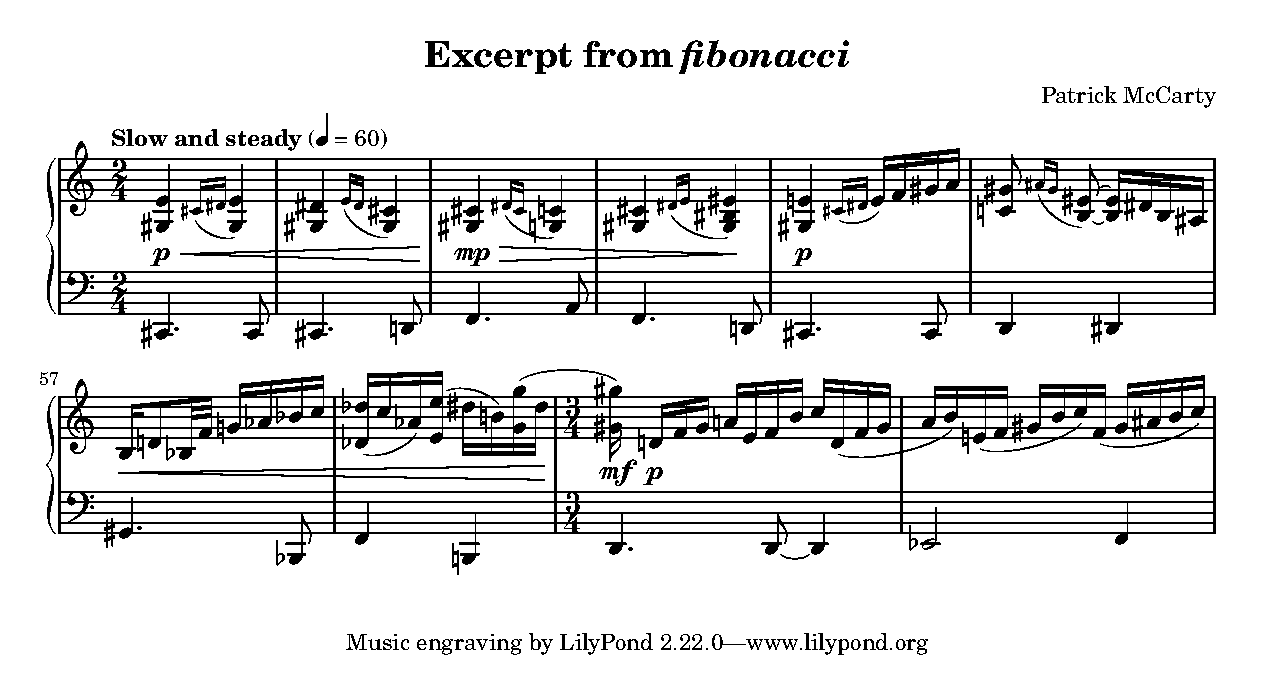
\includegraphics[scale=0.77]{gr-fib.pdf}
\end{VerbatimOut}

\MyIO


  % Physics.
  \ProvidesFile{ap-physics.tex}[2022-10-05 Physics appendix]

\begin{VerbatimOut}{z.out}
\chapter{PHYSICS}
\ix{physics//Physics appendix}

Feynman diagrams\ix{Feynman diagram}
show what happens
when elementary particles collide
\cite{feynman-diagram}.
The Feynman diagrams below are from the
\citetitle{ellis2016} documentation \cite{ellis2016}.
\textbf{%
  You must use \texttt{lualatex} instead
  of \texttt{pdflatex}
  to process documents that use the \texttt{tikz-feynman} package.%
}

The input
in the documentation
is different than here because a different random number generator
is used \cite{menke2019}.
I expect this to be corrected.
In the meantime try replacing \texttt{vertical}
with \texttt{vertical'}
and/or switch some \texttt{fermion}
to \texttt{anti} \texttt{fermion} lines \cite{ellis2017}.
\end{VerbatimOut}

\MyIO


\begin{VerbatimOut}{z.out}
\feynmandiagram [large, vertical'=e to f] {
  a -- [fermion] b -- [photon, momentum=\(k\)] c -- [fermion] d,
  b -- [fermion, momentum'=\(p_{1}\)] e -- [fermion, momentum'=\(p_{2}\)] c,
  e -- [gluon] f,
  h -- [anti fermion] f -- [anti fermion] i,
};
\end{VerbatimOut}

\MyIO


\begin{VerbatimOut}{z.out}
\feynmandiagram [horizontal=a to b] {
  i1 -- [anti fermion] a -- [anti fermion] i2,
  a -- [photon] b,
  f1 -- [fermion] b -- [fermion] f2,
};
\end{VerbatimOut}

\MyIO


  % Notes and footnotes are optional.
  % Reference: TM2017 page 34.
  % I have not implemented this yet.  Mark Senn 2002-06-03

  % A vita is optional for masters theses
  % and required for doctoral dissertations.
  % Reference: TM2017 page 13.
  \ProvidesFile{ap-vita.tex}[2022-10-05 vita appendix]

\begin{vita}
\ix{vita}
\index{\verb+\begin{vita}+}
  
[Put a brief autobiographical sketch here.]

\end{vita}


  % Listing or including publications(s) is optional.
% \ProvidesFile{ap-publications.tex}[2023-06-06 publications appendix]

\ZZnonchapter{odd}{PUBLICATION(S)}{y}{0pt}
\ix{publication environment//publications environment}
\index{\verb+\begin{publicationa}+@\verb+\begin{publication}+}
\index{\verb+\begin{publications}+}
    
The following is based on information in
\cite{template1,template2,template3}.

\renewcommand{\I}{\hspace*{2\ZZparindent}$\bullet$\hspace*{1.5em}}

In a publication or publications section you can\\
  \I list a single publication\index{publication environment}\\
  \I include a single publication\\
  \I list multiple publications\index{publications environment}\\
  \I include multiple publications\\
Use\newline
\hspace*{0.5in}\verb+\begin{publication}+\ldots\verb+\end{publication}+\newline
or\newline
\hspace*{0.5in}\verb+\begin{publications}+\ldots\verb+\end{publications}+\newline
to skip to the next page and put the appropriate heading on the
top of the page.

\vspace*{1.5\baselineskip}

\section*{To Include a Single Publication}

\begin{verbatim}
  \begin{publication}
    ...put a single publication here...
    ...IMPROVE THIS LATER to show how to do that...
  \end{publication}
\end{verbatim}


\section*{To List Publications}

Add\\
\I |keywords = {publication},|\\
to all
|all-biblatex.bib|
entries
that should be in the publications list.

\printbibliography
[
  keywords = {publication},
]


% \includepdf[scale=0.9, pages=1]{ztemp-sgopalsa-paper.pdf}
% \includepdf[offset=-1.5truein 0.25truein, scale=0.9, pages=1]{ztemp-sgopalsa-paper.pdf}
% \includepdf[offset=-1.5truein 0.2truein,  scale=0.9, pages=2]{ztemp-sgopalsa-paper.pdf}
% \includepdf[offset=-1.5truein 0.2truein,  scale=0.9, pages=3]{ztemp-sgopalsa-paper.pdf}
% \includepdf[offset=-1.5truein 0.2truein,  scale=0.9, pages=4]{ztemp-sgopalsa-paper.pdf}
% \includepdf[offset=-1.5truein 0.2truein,  scale=0.9, pages=5]{ztemp-sgopalsa-paper.pdf}
% \includepdf[offset=-1.5truein 0.2truein,  scale=0.9, pages=6]{ztemp-sgopalsa-paper.pdf}
% \includepdf[offset=-1.5truein 0.2truein,  scale=0.9, pages=7]{ztemp-sgopalsa-paper.pdf}

  % Print the index.
  % The index is optional.
  \pdfbookmark{INDEX}{index}
  \printindex

  % If \ZZshowcolophon is true, print the colophon.
  \pdfbookmark{COLOPHON}{colophon}
  \ifthen{\equal{true}{\ZZshowcolophon}}
    {\ProvidesFile{ap-colophon.tex}[2024-09-11 colophon appendix]

\begin{VerbatimOut}{z.out}
\chapter*{COLOPHON}
\label{ap:colophon}
\ix{colophon}

\ExplSyntaxOn
  \ifthen{\equal{true}{\ZZshowcolophon}}
    {
      \sys_if_shell_unrestricted:TF
        % TRUE CODE
        { }
        % FALSE CODE
        {
          \typeout{Consider~using~the~shell-escape~option~so~the}
          \typeout{Biber~version~will~be~included~in~the~colophon.}
          \typeout{Hit~Enter~key~to~continue...}
          \immediate\read15 to \junk
        }
    }
\ExplSyntaxOff

This is the colophon.
A colophon describes how a document was produced \cite{diggypod-colophon}.
This document was compiled on \ZZDateRun\ at \ZZTimeRun\ using
\begin{luacode*}
  local texlive = string.match(tex.luatexbanner, "%((.*)%)")
  tex.sprint(texlive .. ", ")

  local lualatex = tex.luatexbanner
  lualatex = string.gsub(lualatex, "This is ", "")
  lualatex = string.gsub(lualatex, ", Version ", " ")
  lualatex = string.gsub(lualatex, " %(.*", "")
  tex.sprint(lualatex .. ", ")

  local fh = io.popen("biber -v")
  biber = fh:read()
  fh:close()
  biber = string.gsub(biber, "biber version: ", "")
  tex.sprint("Biber " .. biber .. ", ")
\end{luacode*}
and \PurdueThesisVersion.

\begin{tabular}{@{}ll@{}}
  \noalign{\vspace*{6pt}}
  \toprule
  \bfseries Control Sequence& \bfseries Value\\
  \midrule
  \multicolumn{2}{@{}l}{INPUT\hfil}\\
  \verb+\ZZauthor+& \ZZauthor\\
  \verb+\ZZcampus+& \ZZcampus\\
  \verb+\ZZdegree+& \ZZdegree\\
  \verb+\ZZdocument+& \ZZdocument\\
  \verb+\ZZgraduation+& \ZZgraduation\\
  \verb+\ZZinstitution+& \ZZinstitution\\
  \verb+\ZZprogram+& \ZZprogram\\
  \verb+\ZZtitle+& \ZZtitle\\
  \noalign{\vspace*{6pt}}
  \verb+\ZZshowcolophon+& \ZZshowcolophon\\
  \verb+\ZZshowdiagonalline+& \ZZshowdiagonalline\\
  \verb+\ZZshowgridlines+& \ZZshowgridlines\\
  \verb+\ZZshowmarginlines+& \ZZshowmarginlines\\
  \verb+\ZZshowtimestamp+& \ZZshowtimestamp\\
  \verb+\ZZshowtodonotes+& \ZZshowtodonotes\\
  \noalign{\vspace*{12pt}}
  \multicolumn{2}{@{}l}{SHORTENED (for debugging)\hfil}\\
  \verb+\ZZcam+& \ZZcam\\
  \verb+\ZZdeg+& \ZZdeg\\
  \verb+\ZZins+& \ZZins\\
  \verb+\ZZpro+& \ZZpro\\
  \noalign{\vspace*{12pt}}
  \multicolumn{2}{@{}l}{DERIVED (for debugging)\hfil}\\
  \verb+\ZZinscam+& \ZZinscam\\
  \verb+\ZZinscampro+& \ZZinscampro\\
  \verb+\ZZinscamprodeg+& \ZZinscamprodeg\\
  \bottomrule
\end{tabular}
\end{VerbatimOut}

\MyIO


\begin{VerbatimOut}{z.out}
\ExplSyntaxOn
  \str_if_eq:NNTF
    \ZZibibstyle
    \ZZbibstyle
    % TRUE CODE
    {\def\ZZtmpa{\ZZibibstyle}}
    % FALSE CODE
    {\def\ZZtmpa{\ZZibibstyle\space overridden~with~\ZZbibstyle}}
  \str_if_eq:NNTF
    \ZZicitestyle
    \ZZcitestyle
    % TRUE CODE
    {\def\ZZtmpb{\ZZicitestyle}}
    % FALSE CODE
    {\def\ZZtmpb{\ZZicitestyle\space overridden~with~\ZZcitestyle}}
\ExplSyntaxOff
\begin{tabular}{@{}ll@{}}
  \noalign{\vspace*{6pt}}
  \toprule
  \bfseries What& \bfseries Value\\
  \midrule
  \verb+bibstyle+& \ZZtmpa\\
  \verb+citestyle+& \ZZtmpb\\
  \bottomrule
\end{tabular}
\end{VerbatimOut}

\MyIO




}

% LaTeX won't read after the \end{document} command.
% You can put notes to yourself or LaTeX input not
% ready for use after "\end{document}" if you'd like.
\end{document}
